\section{Optimizer Families}
\label{sec:annex-optimizers}

\subsection{The Evolution of Optimization in Neural Networks}
The optimizer survey frames transformer optimization as a response to three structural pressures: non-convex loss landscapes, severe curvature heterogeneity across parameter blocks, and the memory cost of storing optimizer state for very large models. The report argues that the field has diverged into several trajectories: adaptive first-order baselines, variance-reduction methods, memory-efficient methods, structured second-order preconditioners, schedule-free methods, and orthogonality-oriented updates.

\subsection{Standard Baseline and Adaptive Optimizers}
\paragraph{SGD with Momentum.}
\begin{figure}[H]
\centering
\fitfigure{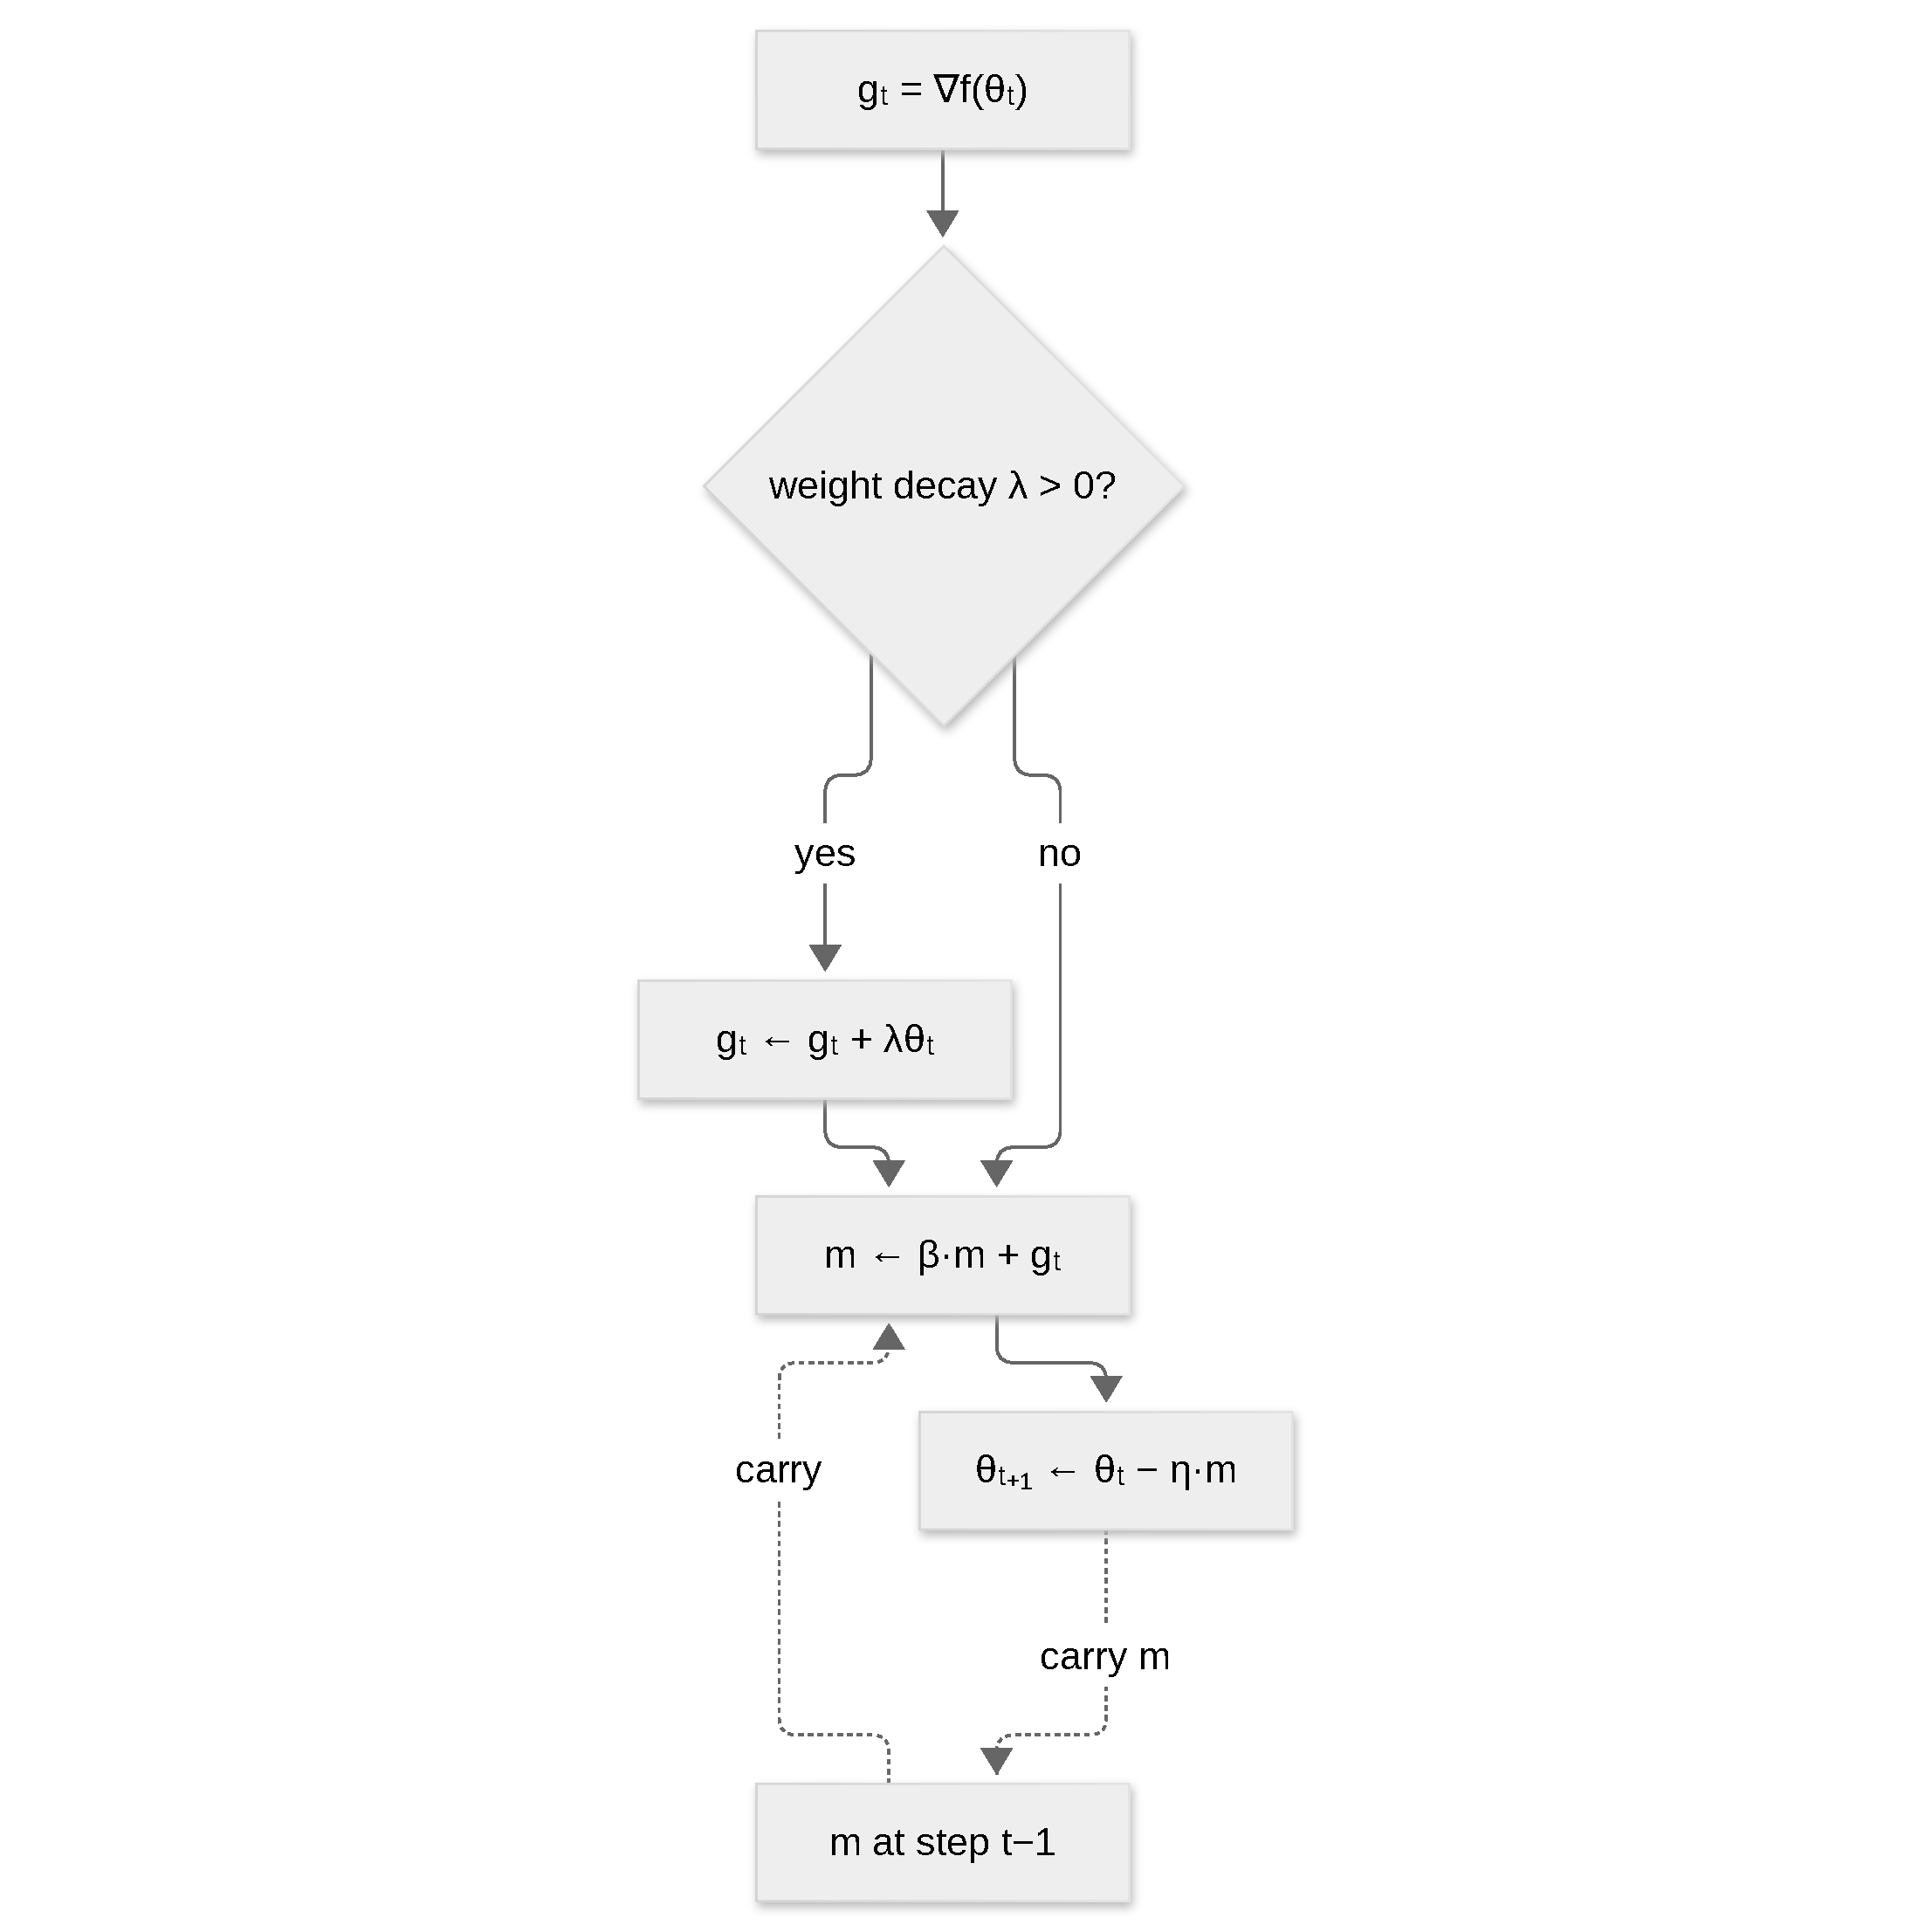
\includegraphics{figures/optimizers/sgd-momentum.pdf}}
\caption{Step flow of SGD with momentum: optional L2 weight decay, exponential momentum accumulation, and the fixed-step parameter update.}
\label{fig:opt-sgd-momentum}
\end{figure}
The classical update accumulates a momentum buffer and then applies a fixed learning rate. At each iteration $t$, the algorithm maintains an exponential moving average $m_t$ of past gradients:
\begin{align}
m_t &= \beta m_{t-1} + g_t \\
\theta_{t+1} &= \theta_t - \eta m_t
\end{align}
where $g_t = \nabla f(\theta_t)$, $\beta \in [0.8, 0.99]$ controls the momentum decay, and $\eta$ is the fixed learning rate. The momentum term acts as velocity: it accelerates movement in consistent directions while dampening oscillations in variable directions.

\begin{algorithm}[H]
\caption{SGD with Momentum}
\label{alg:sgd-momentum}
\begin{algorithmic}[1]
\Require Initial parameters $\theta_0$, learning rate $\eta$, momentum coefficient $\beta$, weight decay $\lambda$
\Ensure Updated parameters $\theta_T$
\State Initialize: momentum buffer $m \gets 0$
\For{$t = 0, 1, 2, \ldots, T-1$}
    \State Compute gradient: $g_t \gets \nabla f(\theta_t)$
    \If{weight\_decay $> 0$}
        \State $g_t \gets g_t + \lambda \theta_t$ \Comment{L2 regularization}
    \EndIf
    \State Update momentum: $m \gets \beta \cdot m + g_t$
    \State Update parameters: $\theta_{t+1} \gets \theta_t - \eta \cdot m$
\EndFor
\Return $\theta_T$
\end{algorithmic}
\end{algorithm}

\paragraph{Cons.}
\begin{itemize}[leftmargin=*]
\item Poor robustness to heterogeneous curvature: a single global rate cannot suit every parameter group.
\item Strong dependence on carefully engineered learning-rate schedules.
\end{itemize}

\paragraph{Pros.}
\begin{itemize}[leftmargin=*]
\item Low memory overhead: a single momentum buffer per parameter.
\item Strong generalization when tuned carefully, and a simple update to implement.
\end{itemize}

\paragraph{Adam and AdamW.}
\begin{figure}[H]
\centering
\fitfigure{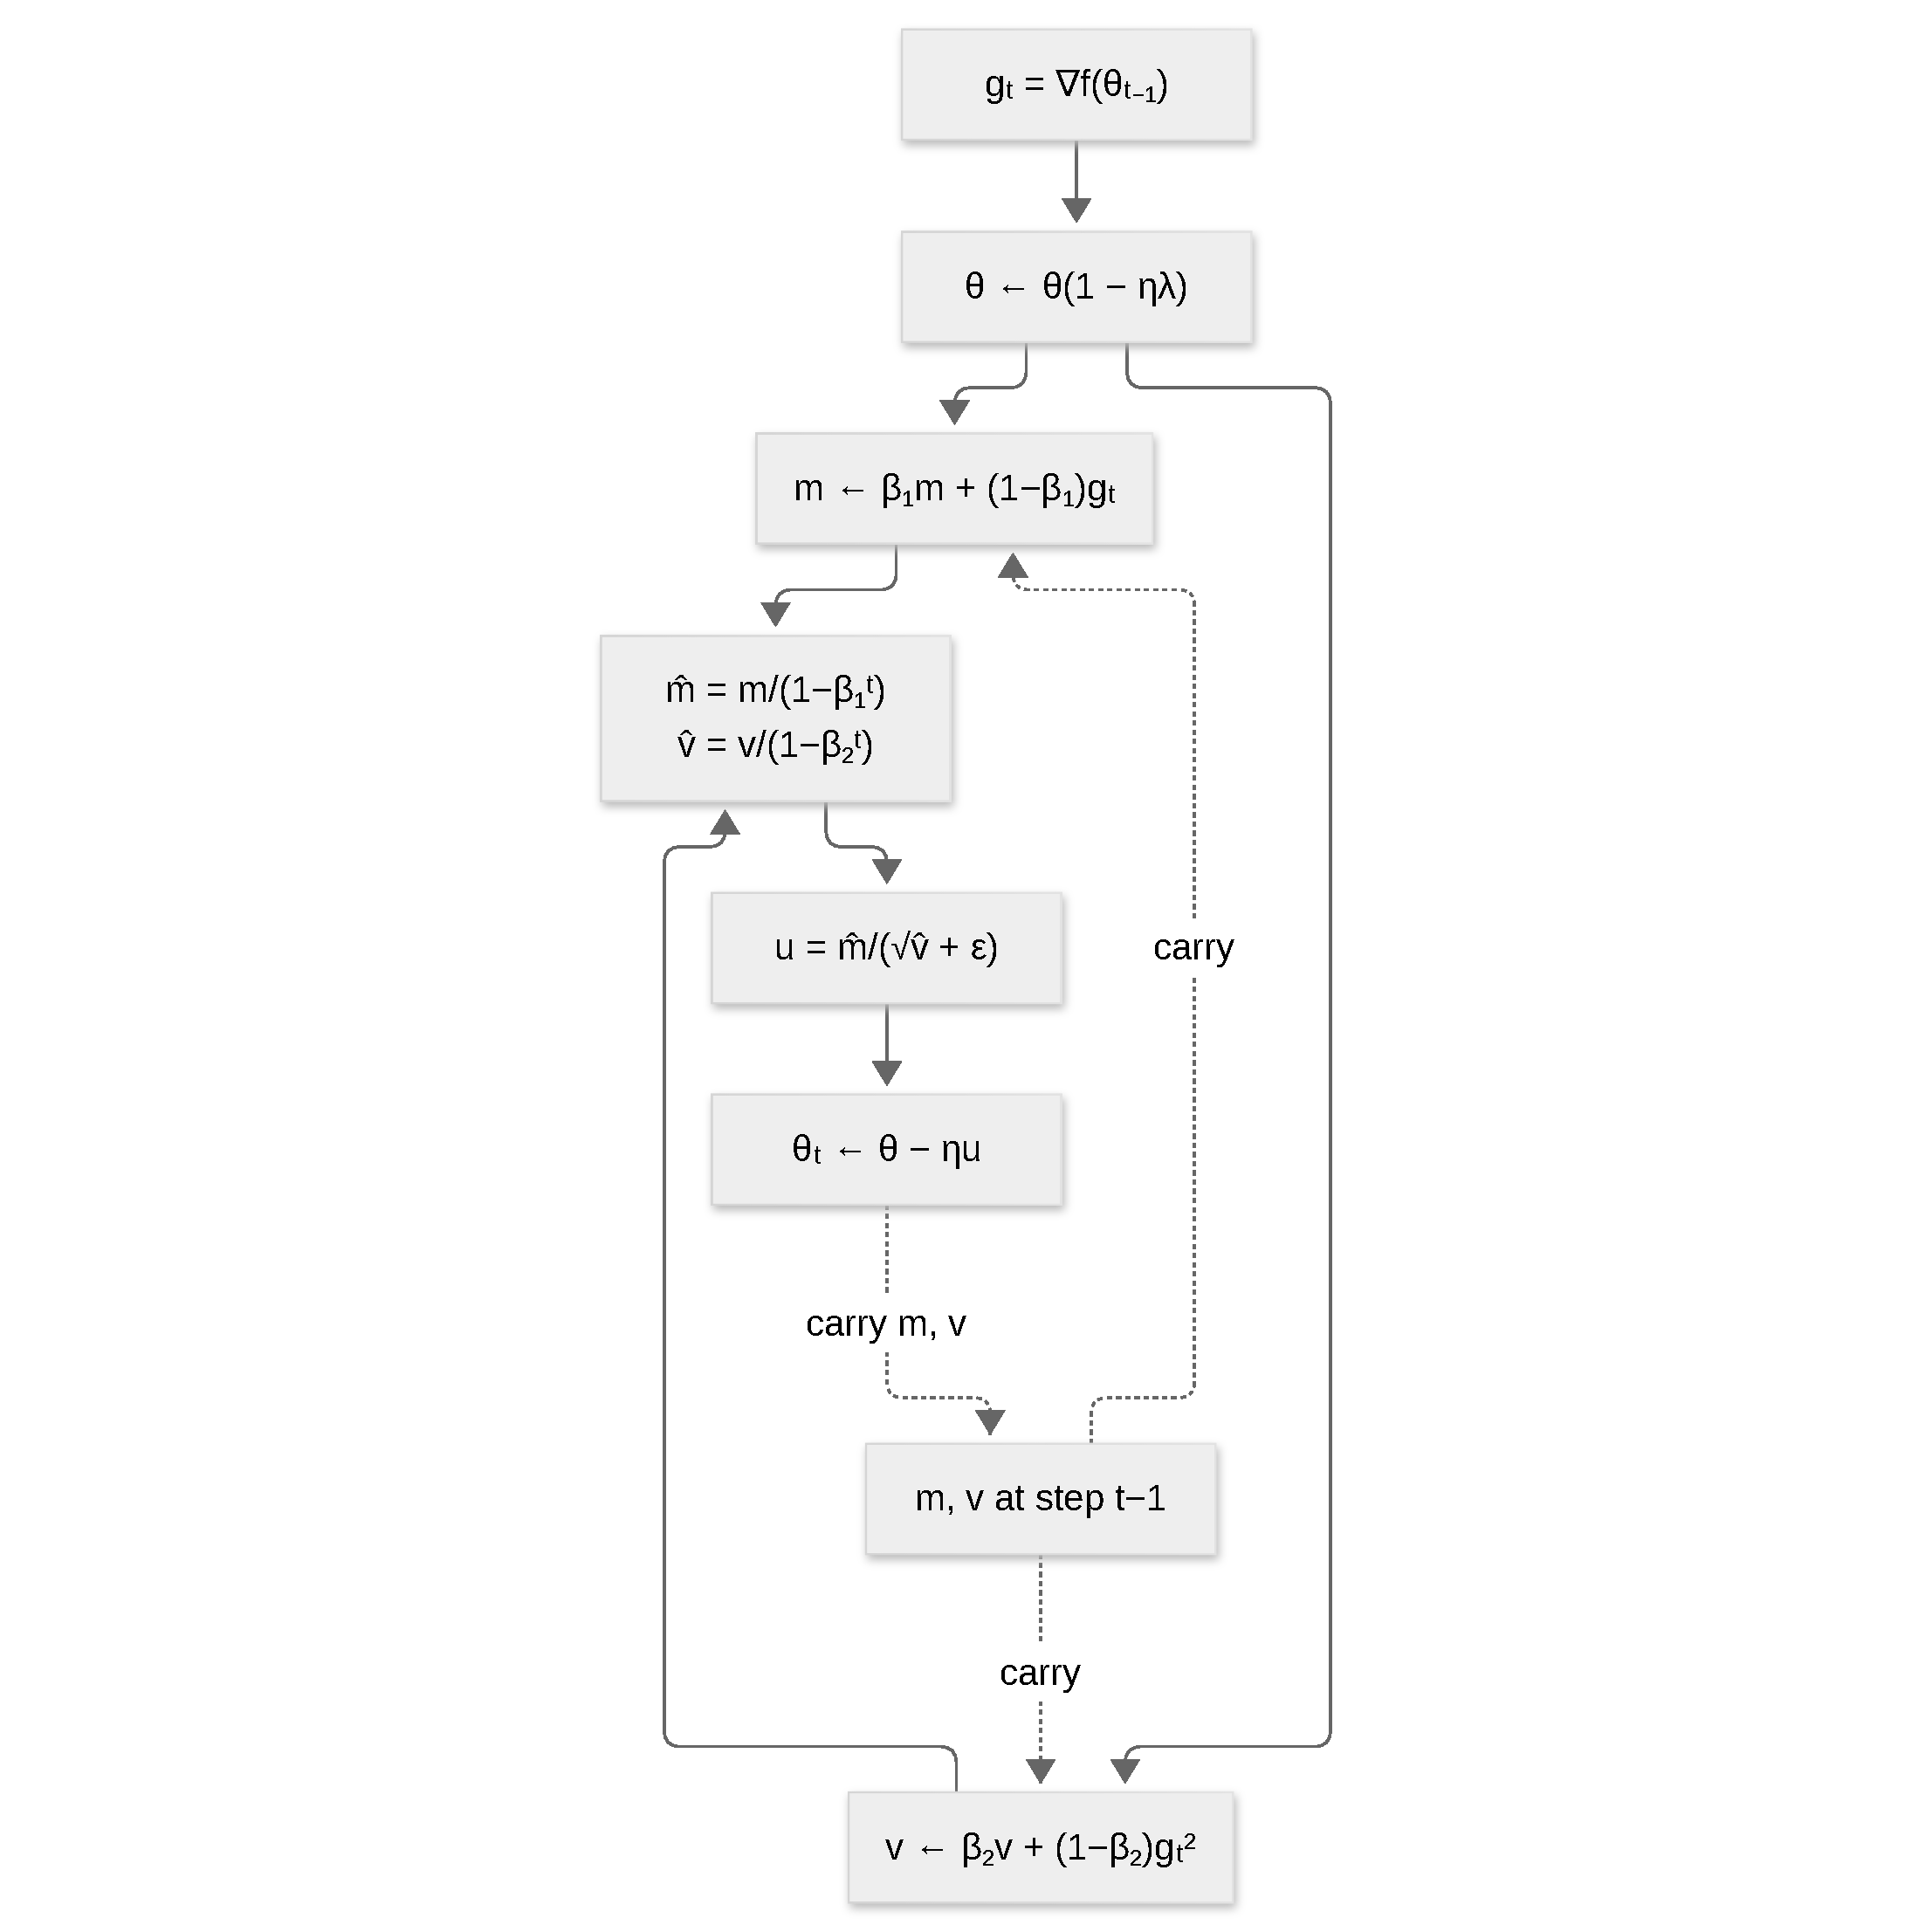
\includegraphics{figures/optimizers/adamw.pdf}}
\caption{Step flow of AdamW: decoupled weight decay, first- and second-moment EMAs, bias correction, and the element-wise adaptive update.}
\label{fig:opt-adamw}
\end{figure}
Adam tracks exponential moving averages of both first moment (mean) and second moment (uncentered variance) to achieve element-wise adaptive learning rates. The update rule is:
\begin{align}
m_t &= \beta_1 m_{t-1} + (1-\beta_1) g_t \\
v_t &= \beta_2 v_{t-1} + (1-\beta_2) g_t^2 \\
\hat{m}_t &= \frac{m_t}{1-\beta_1^t}, \quad \hat{v}_t = \frac{v_t}{1-\beta_2^t} \quad \text{(bias correction)} \\
\theta_{t+1} &= \theta_t - \eta \left(\frac{\hat{m}_t}{\sqrt{\hat{v}_t}+\epsilon}\right)
\end{align}
AdamW introduces a crucial modification: weight decay is applied directly to parameters (decoupled from gradients): $\theta_t \gets \theta_t(1-\eta\lambda)$ rather than adding $\lambda\theta_t$ to the gradient. This decoupling prevents the adaptive scaling from interfering with regularization strength.

\begin{algorithm}[H]
\caption{AdamW (Adam with Decoupled Weight Decay)}
\label{alg:adamw}
\begin{algorithmic}[1]
\Require Initial parameters $\theta_0$, learning rate $\eta$, exponential decay rates $\beta_1, \beta_2 \in [0,1)$
\Require Momentum constant $\epsilon$, weight decay $\lambda$
\Ensure Updated parameters $\theta_T$
\State Initialize: first moment $m \gets 0$, second moment $v \gets 0$, step counter $t \gets 0$
\For{$t = 1, 2, \ldots, T$}
    \State Compute gradient: $g_t \gets \nabla f(\theta_{t-1})$
    \State Weight decay (decoupled): $\theta_{t-1} \gets \theta_{t-1}(1 - \eta\lambda)$
    \State Update moments: $m \gets \beta_1 m + (1-\beta_1) g_t$
    \State $v \gets \beta_2 v + (1-\beta_2) g_t^2$
    \State Bias correction: $\hat{m} \gets m / (1 - \beta_1^t)$, $\hat{v} \gets v / (1 - \beta_2^t)$
    \State Update parameters: $\theta_t \gets \theta_{t-1} - \eta (\hat{m} / (\sqrt{\hat{v}} + \epsilon))$
\EndFor
\Return $\theta_T$
\end{algorithmic}
\end{algorithm}

\paragraph{Cons.}
\begin{itemize}[leftmargin=*]
\item Stores first and second moment tensors for every parameter, doubling optimizer-state memory relative to SGD.
\item Element-wise adaptive scaling can interfere with regularization unless weight decay is decoupled.
\end{itemize}

\paragraph{Pros.}
\begin{itemize}[leftmargin=*]
\item Practical baseline for transformer fine-tuning: fast convergence and forgiving to hyperparameter variation.
\item Decoupled weight decay keeps the regularization strength independent of the adaptive scaling.
\end{itemize}

\paragraph{RAdam (Rectified Adam).}
\begin{figure}[H]
\centering
\fitfigure{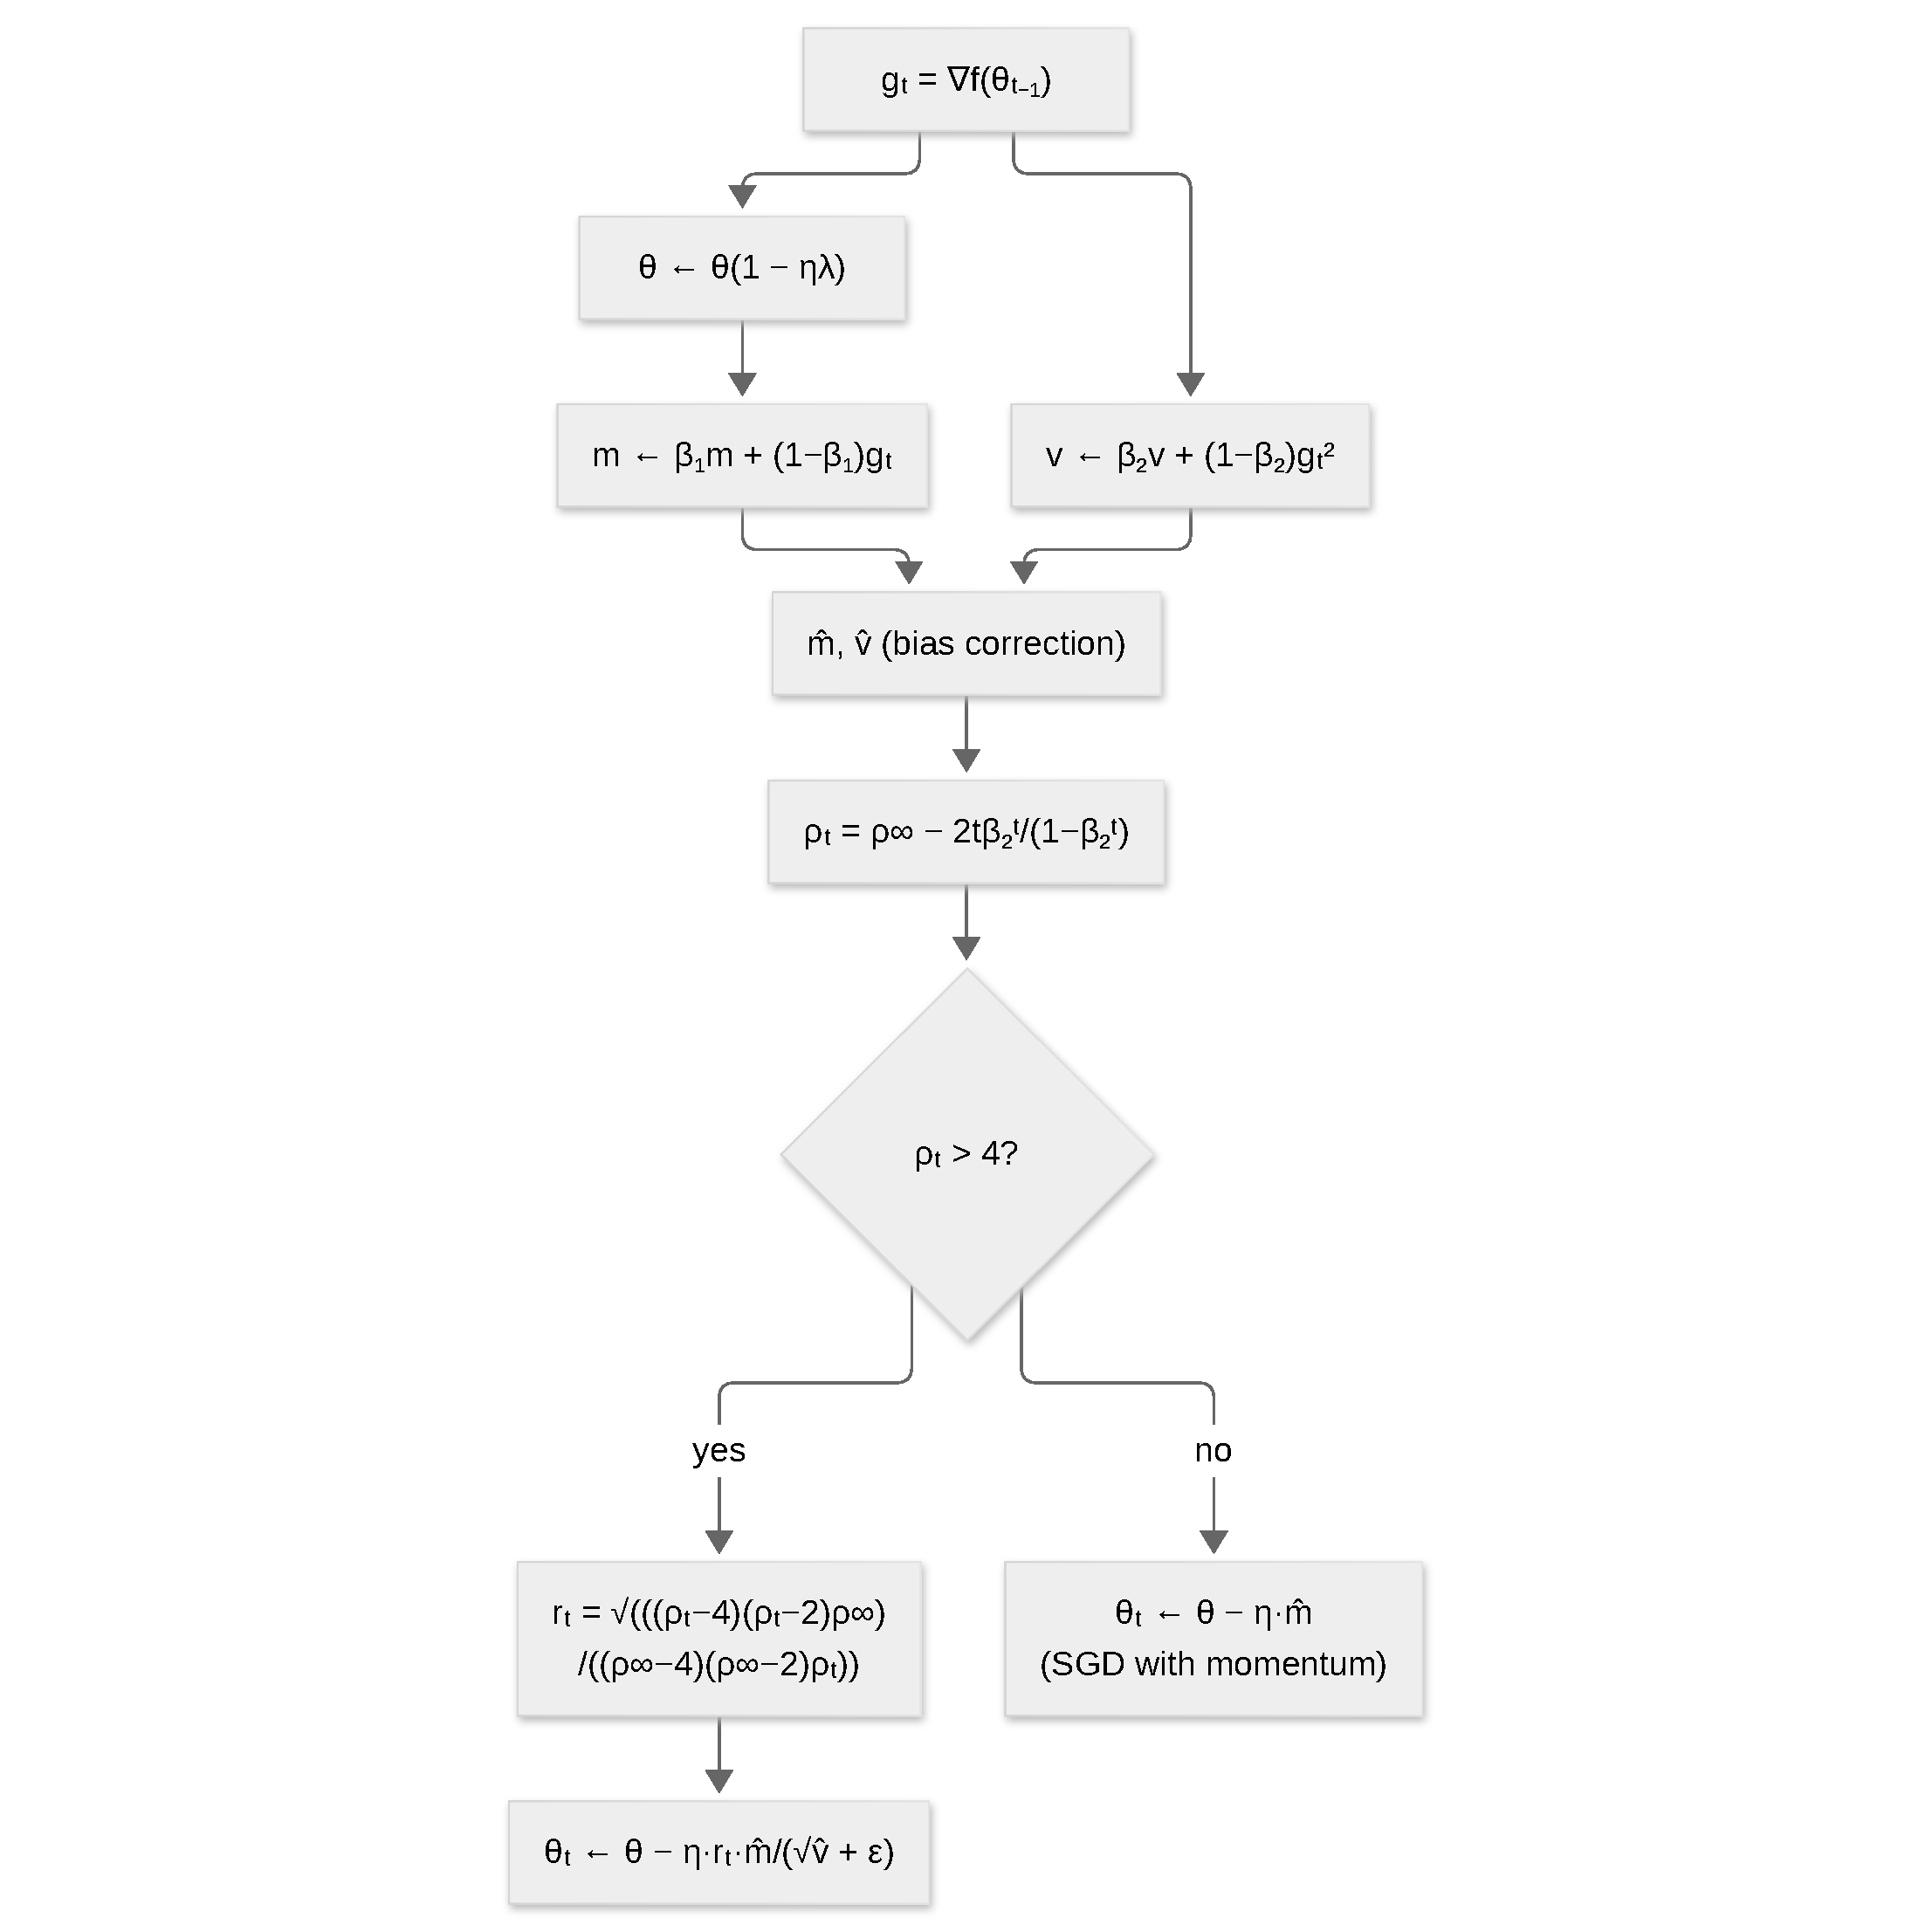
\includegraphics{figures/optimizers/radam.pdf}}
\caption{Step flow of RAdam: SMA-window rectification with an early-step fallback to momentum SGD.}
\label{fig:opt-radam}
\end{figure}
RAdam addresses Adam's instability in early training by dynamically rectifying the adaptive learning rate. The key observation is that the second moment $v_t$ has very high variance in the first few steps, causing unreliable adaptive scaling. RAdam computes the effective simple moving average (SMA) window length:
\[\rho_t = \rho_{\infty} - \frac{2t\beta_2^t}{1-\beta_2^t}, \quad \text{where} \quad \rho_{\infty} = \frac{2}{1-\beta_2}-1\]
When $\rho_t > 4$ (sufficient samples for variance estimation), RAdam applies adaptive scaling with a rectification term:
\[r_t = \sqrt{\frac{(\rho_t-4)(\rho_t-2)\rho_{\infty}}{(\rho_{\infty}-4)(\rho_{\infty}-2)\rho_t}}, \quad \theta_{t+1} = \theta_t - \eta r_t \frac{\hat{m}_t}{\sqrt{\hat{v}_t}+\epsilon}\]
When $\rho_t \leq 4$, RAdam falls back to SGD with momentum: $\theta_{t+1} = \theta_t - \eta\hat{m}_t$.

\begin{algorithm}[H]
\caption{RAdam (Rectified Adam)}
\label{alg:radam}
\begin{algorithmic}[1]
\Require Initial parameters $\theta_0$, learning rate $\eta$, $\beta_1, \beta_2$, weight decay $\lambda$
\Ensure Updated parameters $\theta_T$
\State Initialize: $m \gets 0$, $v \gets 0$, $t \gets 0$
\State Compute: $\rho_\infty \gets 2/(1-\beta_2) - 1$
\For{$t = 1, 2, \ldots, T$}
    \State $g_t \gets \nabla f(\theta_{t-1})$
    \If{weight\_decay $> 0$}
        \State $\theta_{t-1} \gets \theta_{t-1}(1 - \eta\lambda)$
    \EndIf
    \State $m \gets \beta_1 m + (1-\beta_1) g_t$
    \State $v \gets \beta_2 v + (1-\beta_2) g_t^2$
    \State $\hat{m} \gets m/(1-\beta_1^t)$, $\hat{v} \gets v/(1-\beta_2^t)$
    \State $\rho_t \gets \rho_\infty - 2t \beta_2^t / (1 - \beta_2^t)$
    \If{$\rho_t > 4$}
        \State $r_t \gets \sqrt{((\rho_t-4)(\rho_t-2)\rho_\infty) / ((\rho_\infty-4)(\rho_\infty-2)\rho_t)}$
        \State $\theta_t \gets \theta_{t-1} - \eta r_t \hat{m} / (\sqrt{\hat{v}} + \epsilon)$
    \Else
        \State $\theta_t \gets \theta_{t-1} - \eta \hat{m}$ \Comment{SGD with momentum}
    \EndIf
\EndFor
\Return $\theta_T$
\end{algorithmic}
\end{algorithm}

\paragraph{Cons.}
\begin{itemize}[leftmargin=*]
\item Adds rectification bookkeeping on top of Adam's moment state.
\item The benefit shrinks when a well-tuned warmup schedule is already in use.
\end{itemize}

\paragraph{Pros.}
\begin{itemize}[leftmargin=*]
\item Eliminates the need for manual learning-rate warmup by rectifying the adaptive rate.
\item Falls back gracefully to momentum SGD while variance estimates are unreliable, improving robustness.
\end{itemize}

\subsection{Advanced Momentum and Variance Reduction (2024--2025)}
\paragraph{Adan (Adaptive Nesterov Momentum).}
\begin{figure}[H]
\centering
\fitfigure{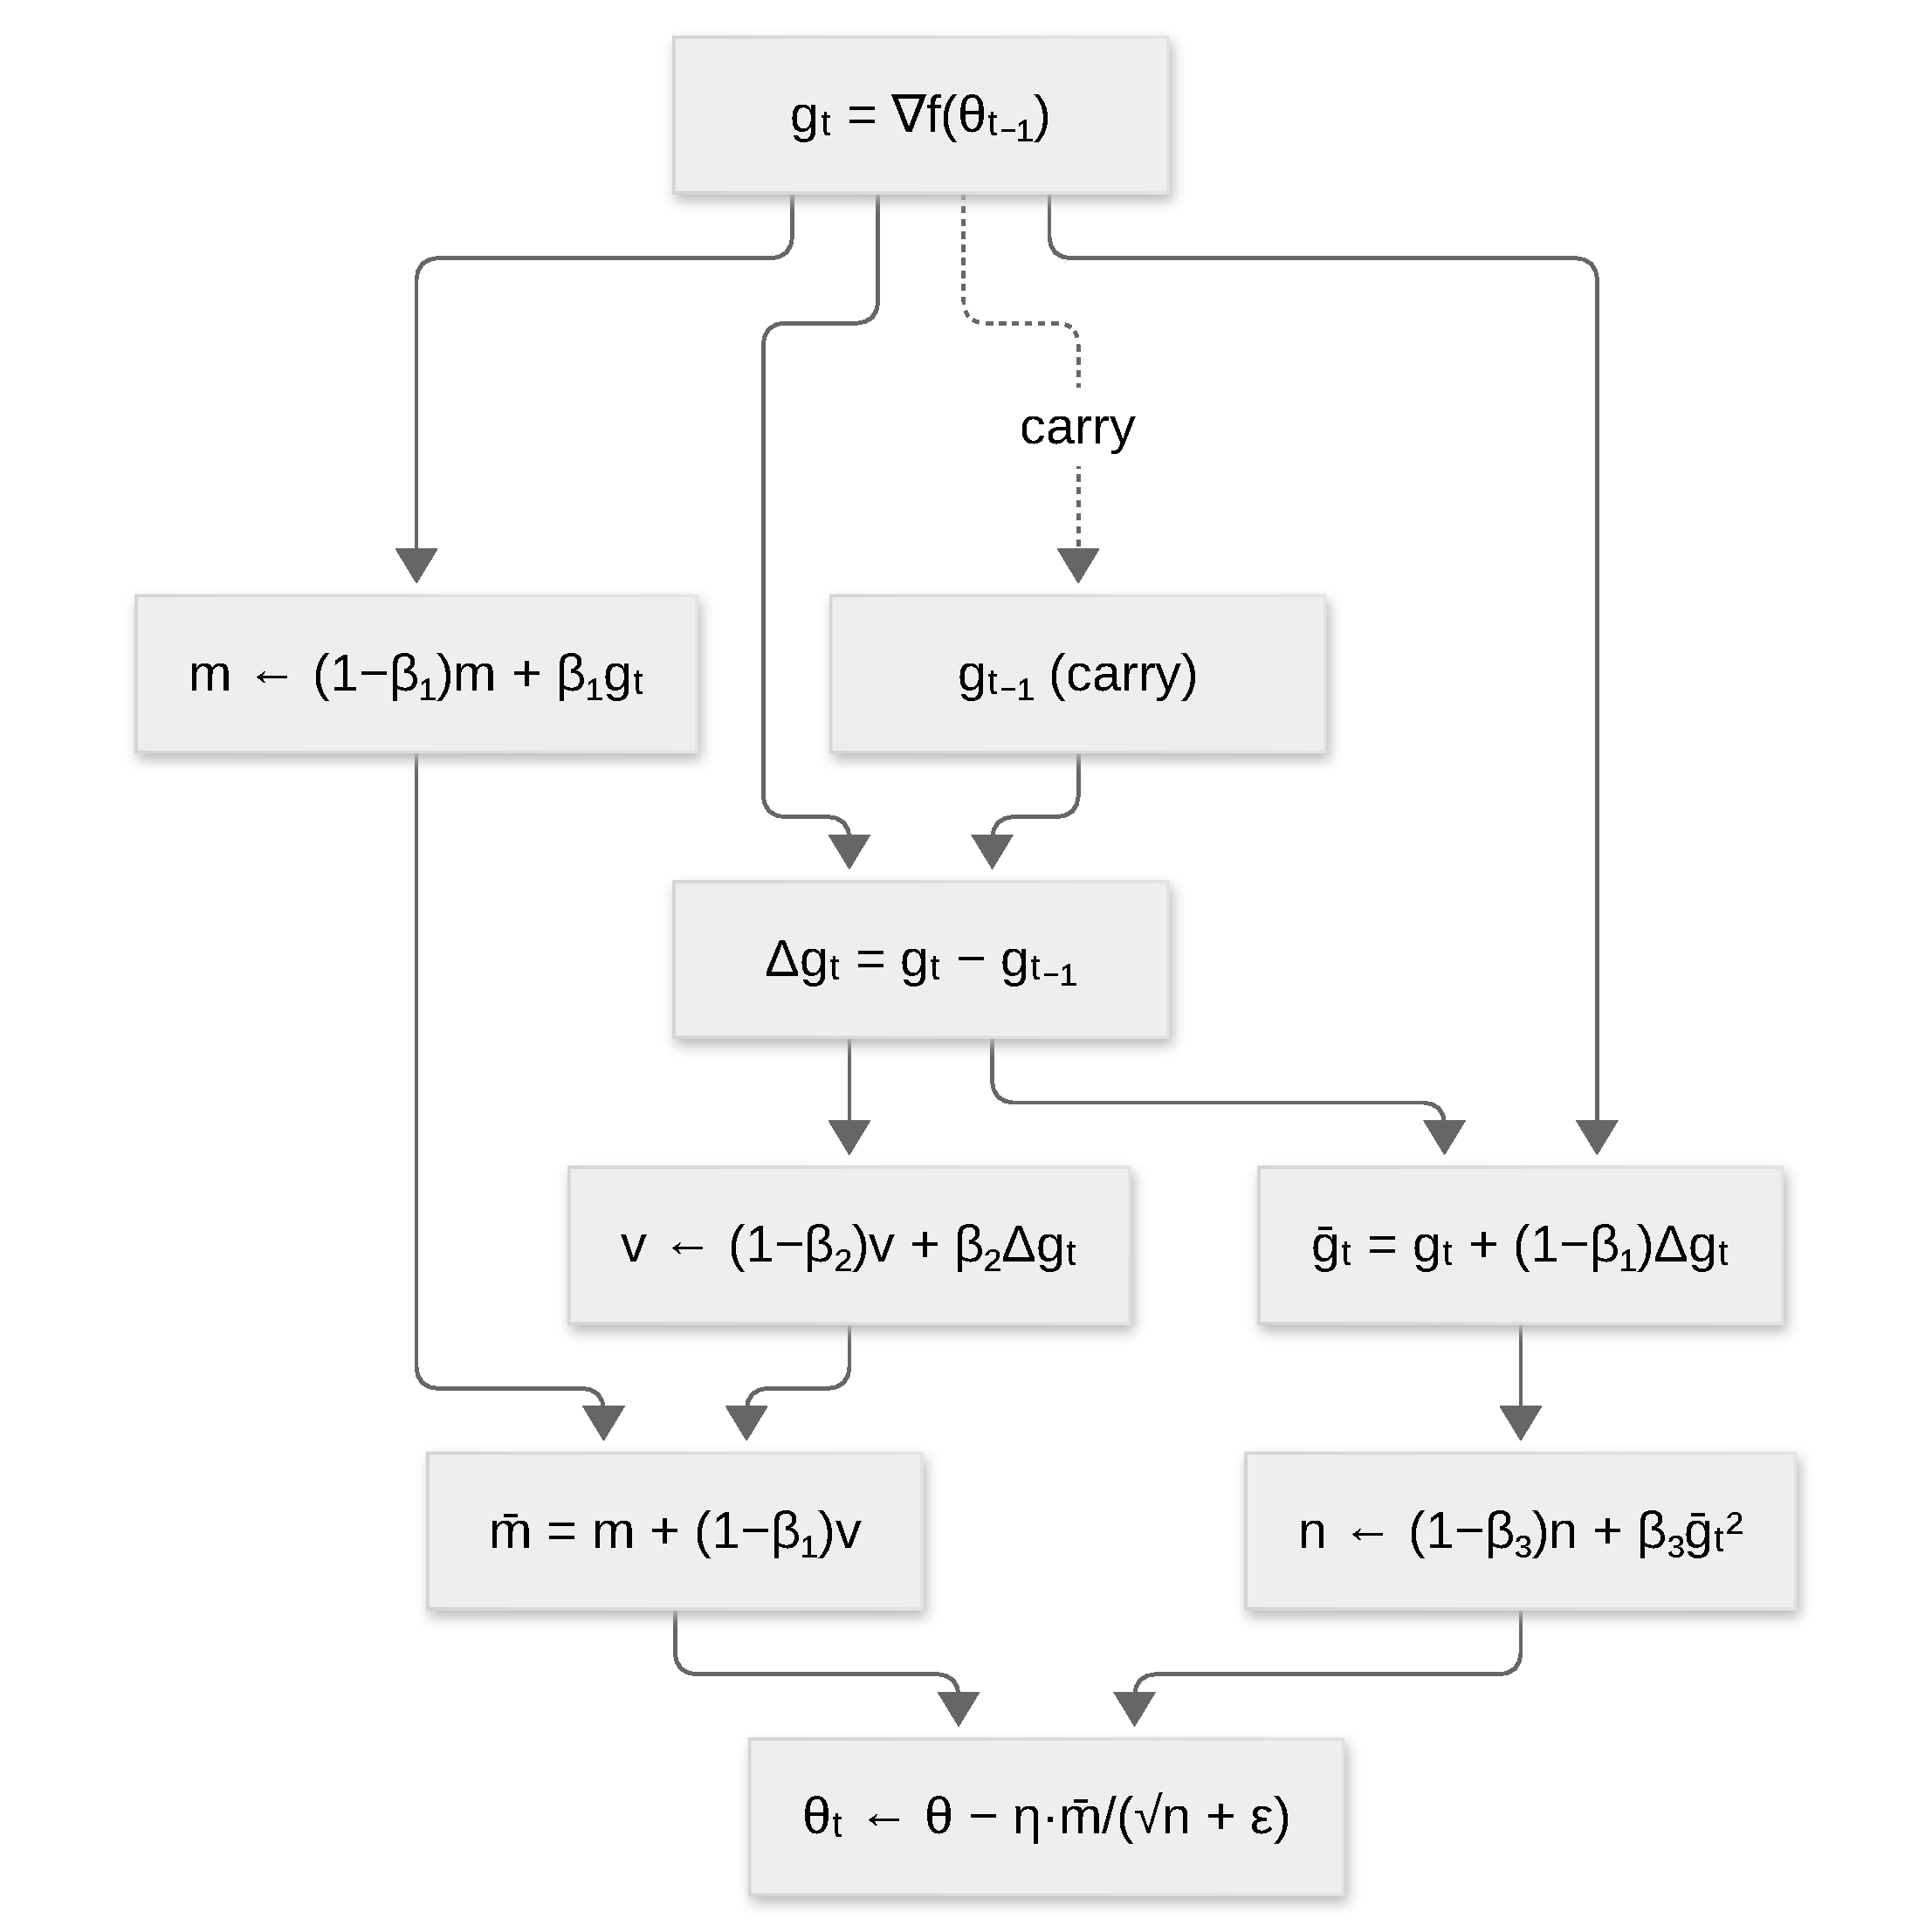
\includegraphics{figures/optimizers/adan.pdf}}
\caption{Step flow of Adan: Nesterov momentum estimation from the gradient difference, with three state buffers and a combined momentum step.}
\label{fig:opt-adan}
\end{figure}
Adan reformulates Nesterov acceleration without the extra gradient computation required by classical Nesterov SGD. The algorithm maintains three momentum buffers:
\begin{align}
m_t &= (1-\beta_1)m_{t-1} + \beta_1 g_t \quad\text{(first moment)} \\
v_t &= (1-\beta_2)v_{t-1} + \beta_2(g_t - g_{t-1}) \quad\text{(velocity/gradient difference)} \\
n_t &= (1-\beta_3)n_{t-1} + \beta_3[g_t + (1-\beta_1)(g_t-g_{t-1})]^2 \quad\text{(Nesterov second moment)}
\end{align}
The \textbf{Nesterov Momentum Estimation} (NME) term $\bar{g}_t = g_t + (1-\beta_1)(g_t-g_{t-1})$ estimates the gradient at a future position without evaluating it. The update combines momentum with velocity:
\[\bar{m}_t = m_t + (1-\beta_1)v_t, \quad \theta_{t+1} = \theta_t - \eta\frac{\bar{m}_t}{\sqrt{n_t}+\epsilon}\]

\begin{algorithm}[H]
\caption{Adan (Adaptive Nesterov Momentum)}
\label{alg:adan}
\begin{algorithmic}[1]
\Require Initial parameters $\theta_0$, learning rate $\eta$, $\beta_1, \beta_2, \beta_3 \in (0,1)$
\Ensure Updated parameters $\theta_T$
\State Initialize: $m \gets 0$, $v \gets 0$, $n \gets 0$, $g_{-1} \gets 0$ (previous gradient)
\For{$t = 1, 2, \ldots, T$}
    \State $g_t \gets \nabla f(\theta_{t-1})$
    \State $m \gets (1-\beta_1) m + \beta_1 g_t$
    \State $\Delta g_t \gets g_t - g_{t-1}$
    \State $v \gets (1-\beta_2) v + \beta_2 \Delta g_t$
    \State Nesterov estimation: $\bar{g}_t \gets g_t + (1-\beta_1) \Delta g_t$
    \State $n \gets (1-\beta_3) n + \beta_3 \bar{g}_t^2$
    \State Combined momentum: $\bar{m} \gets m + (1-\beta_1) v$
    \State $\theta_t \gets \theta_{t-1} - \eta (\bar{m} / (\sqrt{n} + \epsilon))$
    \State $g_{t-1} \gets g_t$
\EndFor
\Return $\theta_T$
\end{algorithmic}
\end{algorithm}

\paragraph{Cons.}
\begin{itemize}[leftmargin=*]
\item Three momentum-like buffers increase memory overhead relative to Adam.
\item Additional gradient-difference bookkeeping per step.
\end{itemize}

\paragraph{Pros.}
\begin{itemize}[leftmargin=*]
\item Nesterov-style acceleration without an extra gradient evaluation.
\item Fast convergence across diverse architectures (CNNs, GANs, transformers).
\end{itemize}

\paragraph{ADOPT (Adam with Optimal Pruned Tuning).}
\begin{figure}[H]
\centering
\fitfigure{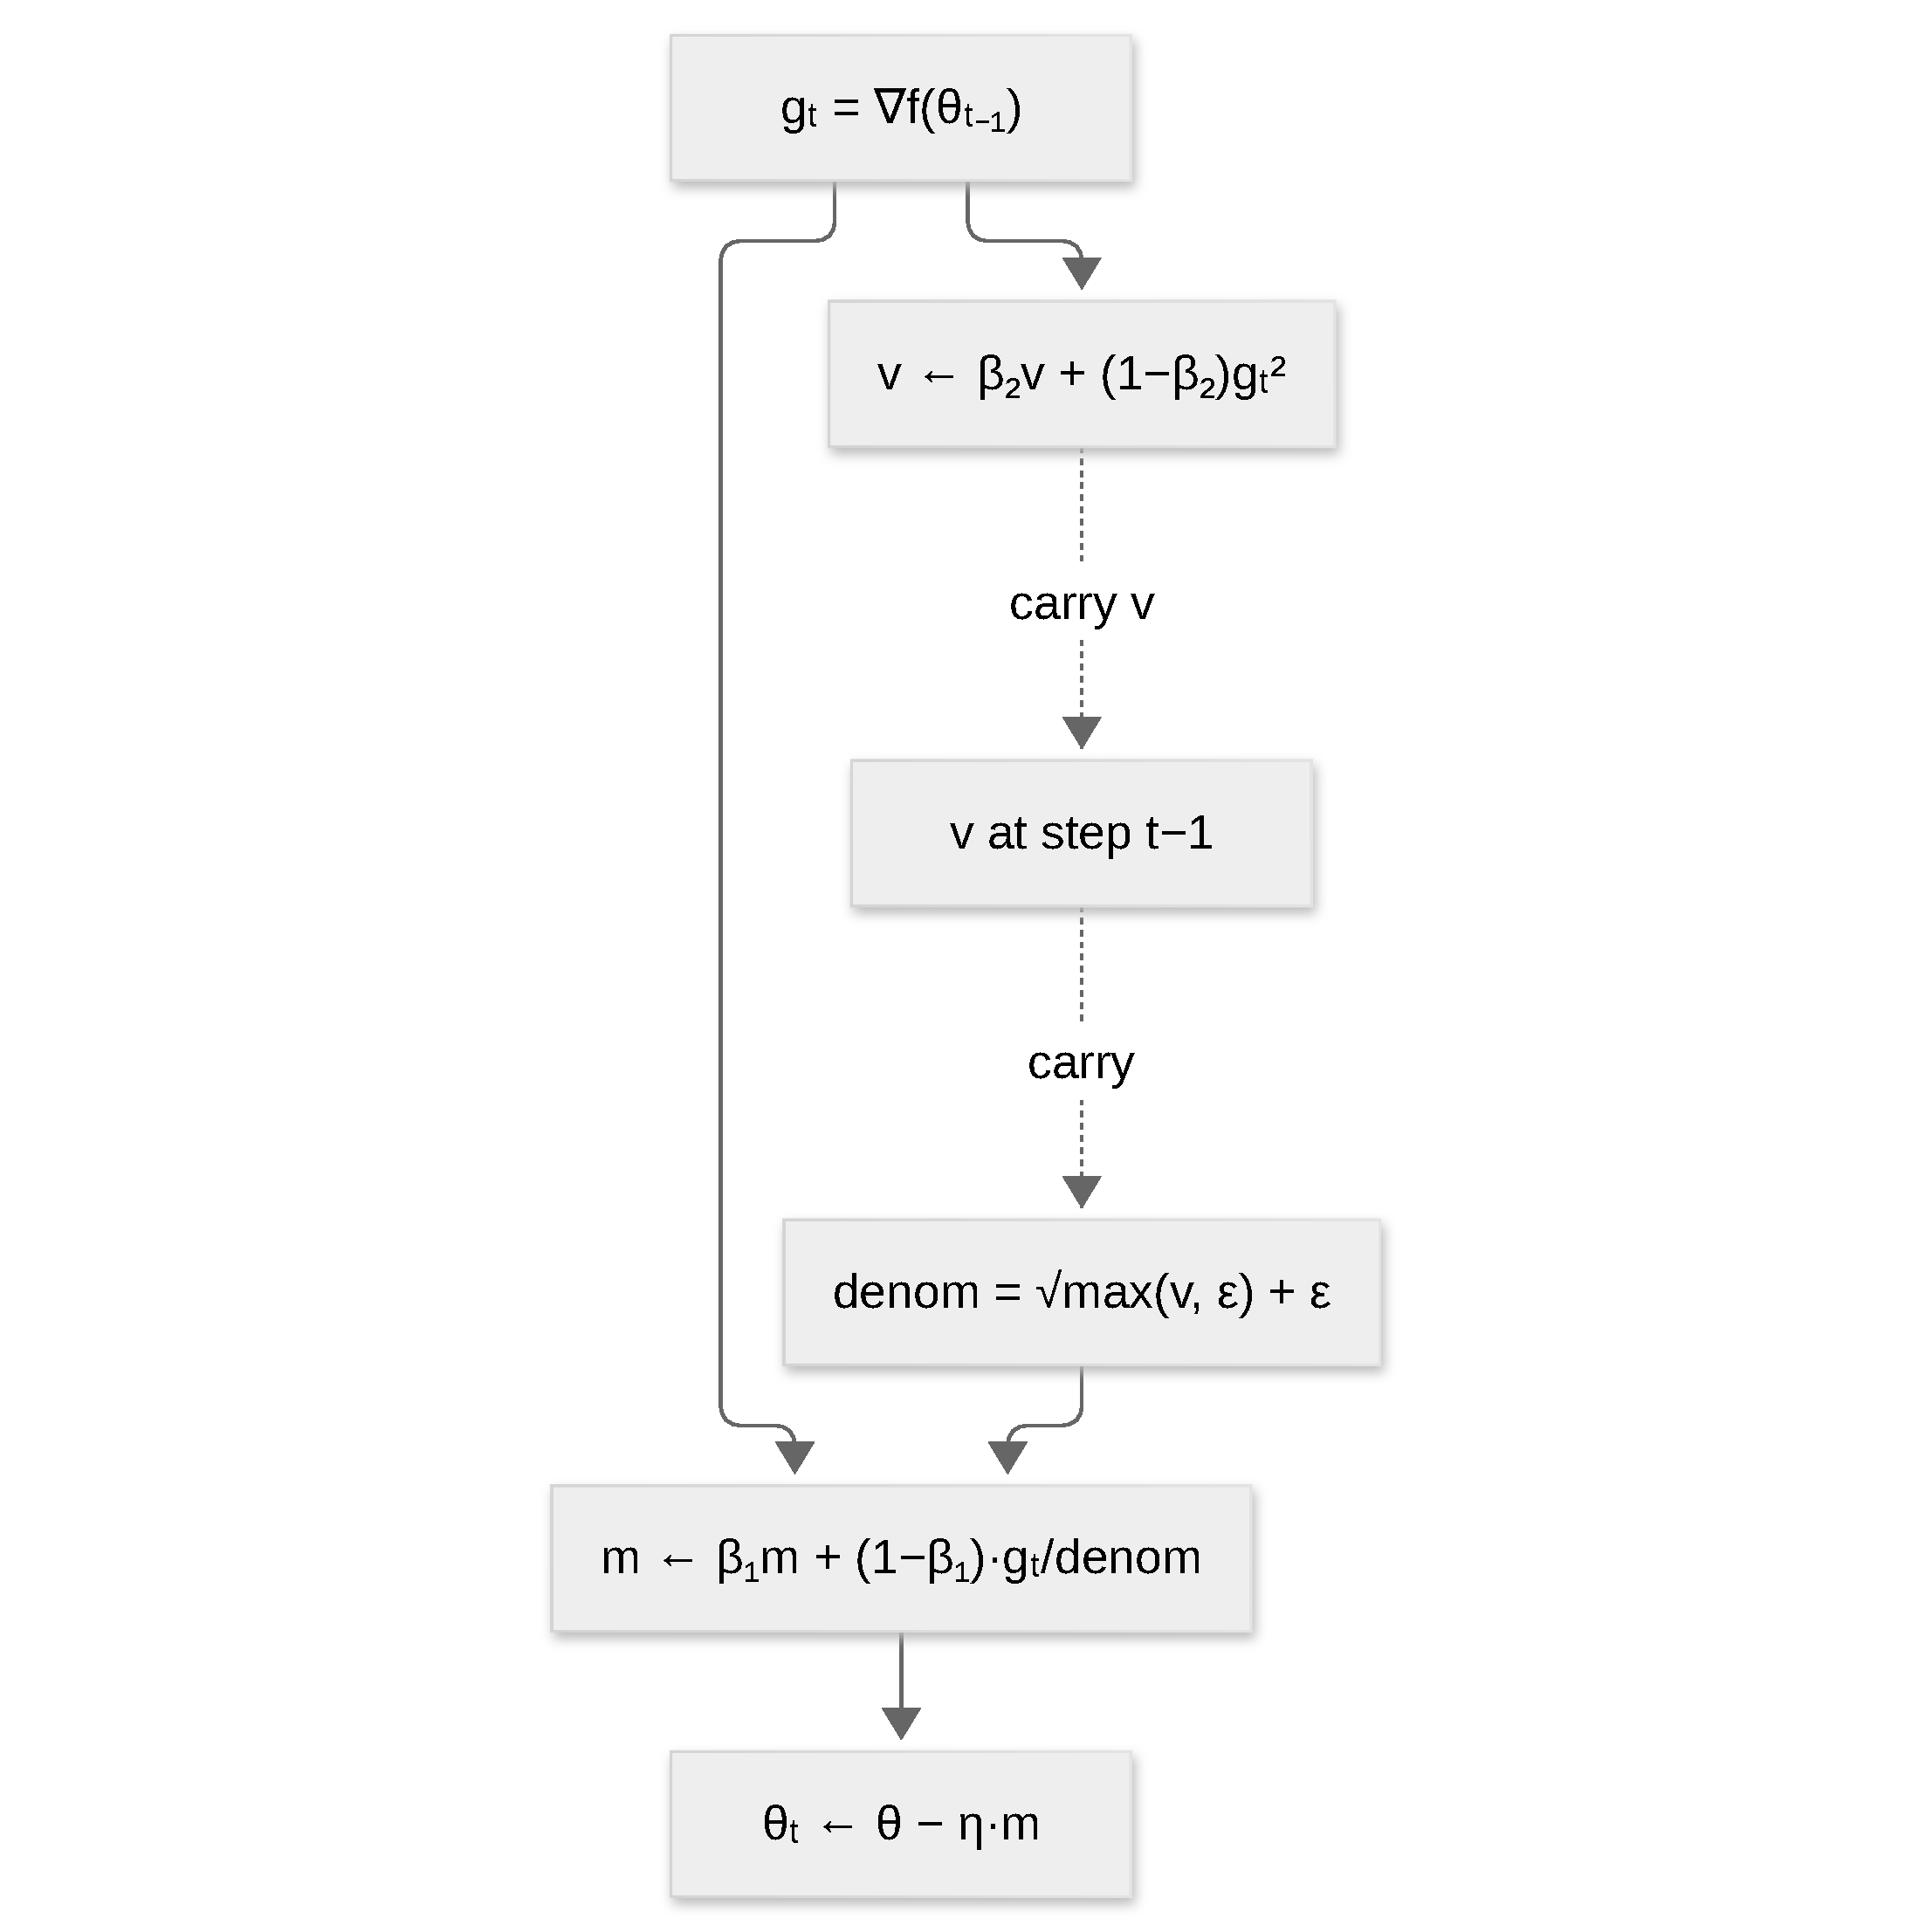
\includegraphics{figures/optimizers/adopt.pdf}}
\caption{Step flow of ADOPT: the second moment from the previous step normalizes the current gradient before the first-moment update.}
\label{fig:opt-adopt}
\end{figure}
ADOPT fixes a fundamental theoretical issue in Adam: the gradient appears in both the first moment and second moment estimates, creating circularity. ADOPT \textbf{decouples} by using the previous step's second moment for the denominator:
\begin{align}
v_t &= \beta_2 v_{t-1} + (1-\beta_2)g_t^2 \\
m_t &= \beta_1 m_{t-1} + (1-\beta_1)\frac{g_t}{\sqrt{v_{t-1}}+\epsilon} \quad\text{(uses $v_{t-1}$, not $v_t$)} \\
\theta_{t+1} &= \theta_t - \eta m_t
\end{align}

\begin{algorithm}[H]
\caption{ADOPT (Adam with Optimal Pruned Tuning)}
\label{alg:adopt}
\begin{algorithmic}[1]
\Require Initial parameters $\theta_0$, learning rate $\eta$, $\beta_1, \beta_2$, tolerance $\epsilon$
\Ensure Updated parameters $\theta_T$
\State Initialize: $m \gets 0$, $v \gets 0$
\For{$t = 1, 2, \ldots, T$}
    \State $g_t \gets \nabla f(\theta_{t-1})$
    \If{weight\_decay $> 0$}
        \State $\theta_{t-1} \gets \theta_{t-1}(1 - \eta\lambda)$
    \EndIf
    \State Use \textbf{previous} second moment: $\text{denom} \gets \sqrt{\max(v, \epsilon)} + \epsilon$
    \State Update first moment using previous variance: $m \gets \beta_1 m + (1-\beta_1)(g_t / \text{denom})$
    \State Update second moment with \textbf{current} gradient: $v \gets \beta_2 v + (1-\beta_2) g_t^2$
    \State $\theta_t \gets \theta_{t-1} - \eta m$
\EndFor
\Return $\theta_T$
\end{algorithmic}
\end{algorithm}

\paragraph{Cons.}
\begin{itemize}[leftmargin=*]
\item Requires keeping the previous second moment as an explicit denominator.
\item Empirical gains are architecture- and tuning-dependent.
\end{itemize}

\paragraph{Pros.}
\begin{itemize}[leftmargin=*]
\item Removes Adam's gradient circularity and attains the optimal convergence rate $O(1/\sqrt{T})$ with \textbf{any} $\beta_2 \in (0,1)$, without bounded-noise assumptions.
\item Drop-in Adam replacement with comparable or superior empirical performance across vision, NLP, RL, and generative modeling.
\end{itemize}

\paragraph{AdEMAMix (Exponential Moving Average Mixture).}
\begin{figure}[H]
\centering
\fitfigure{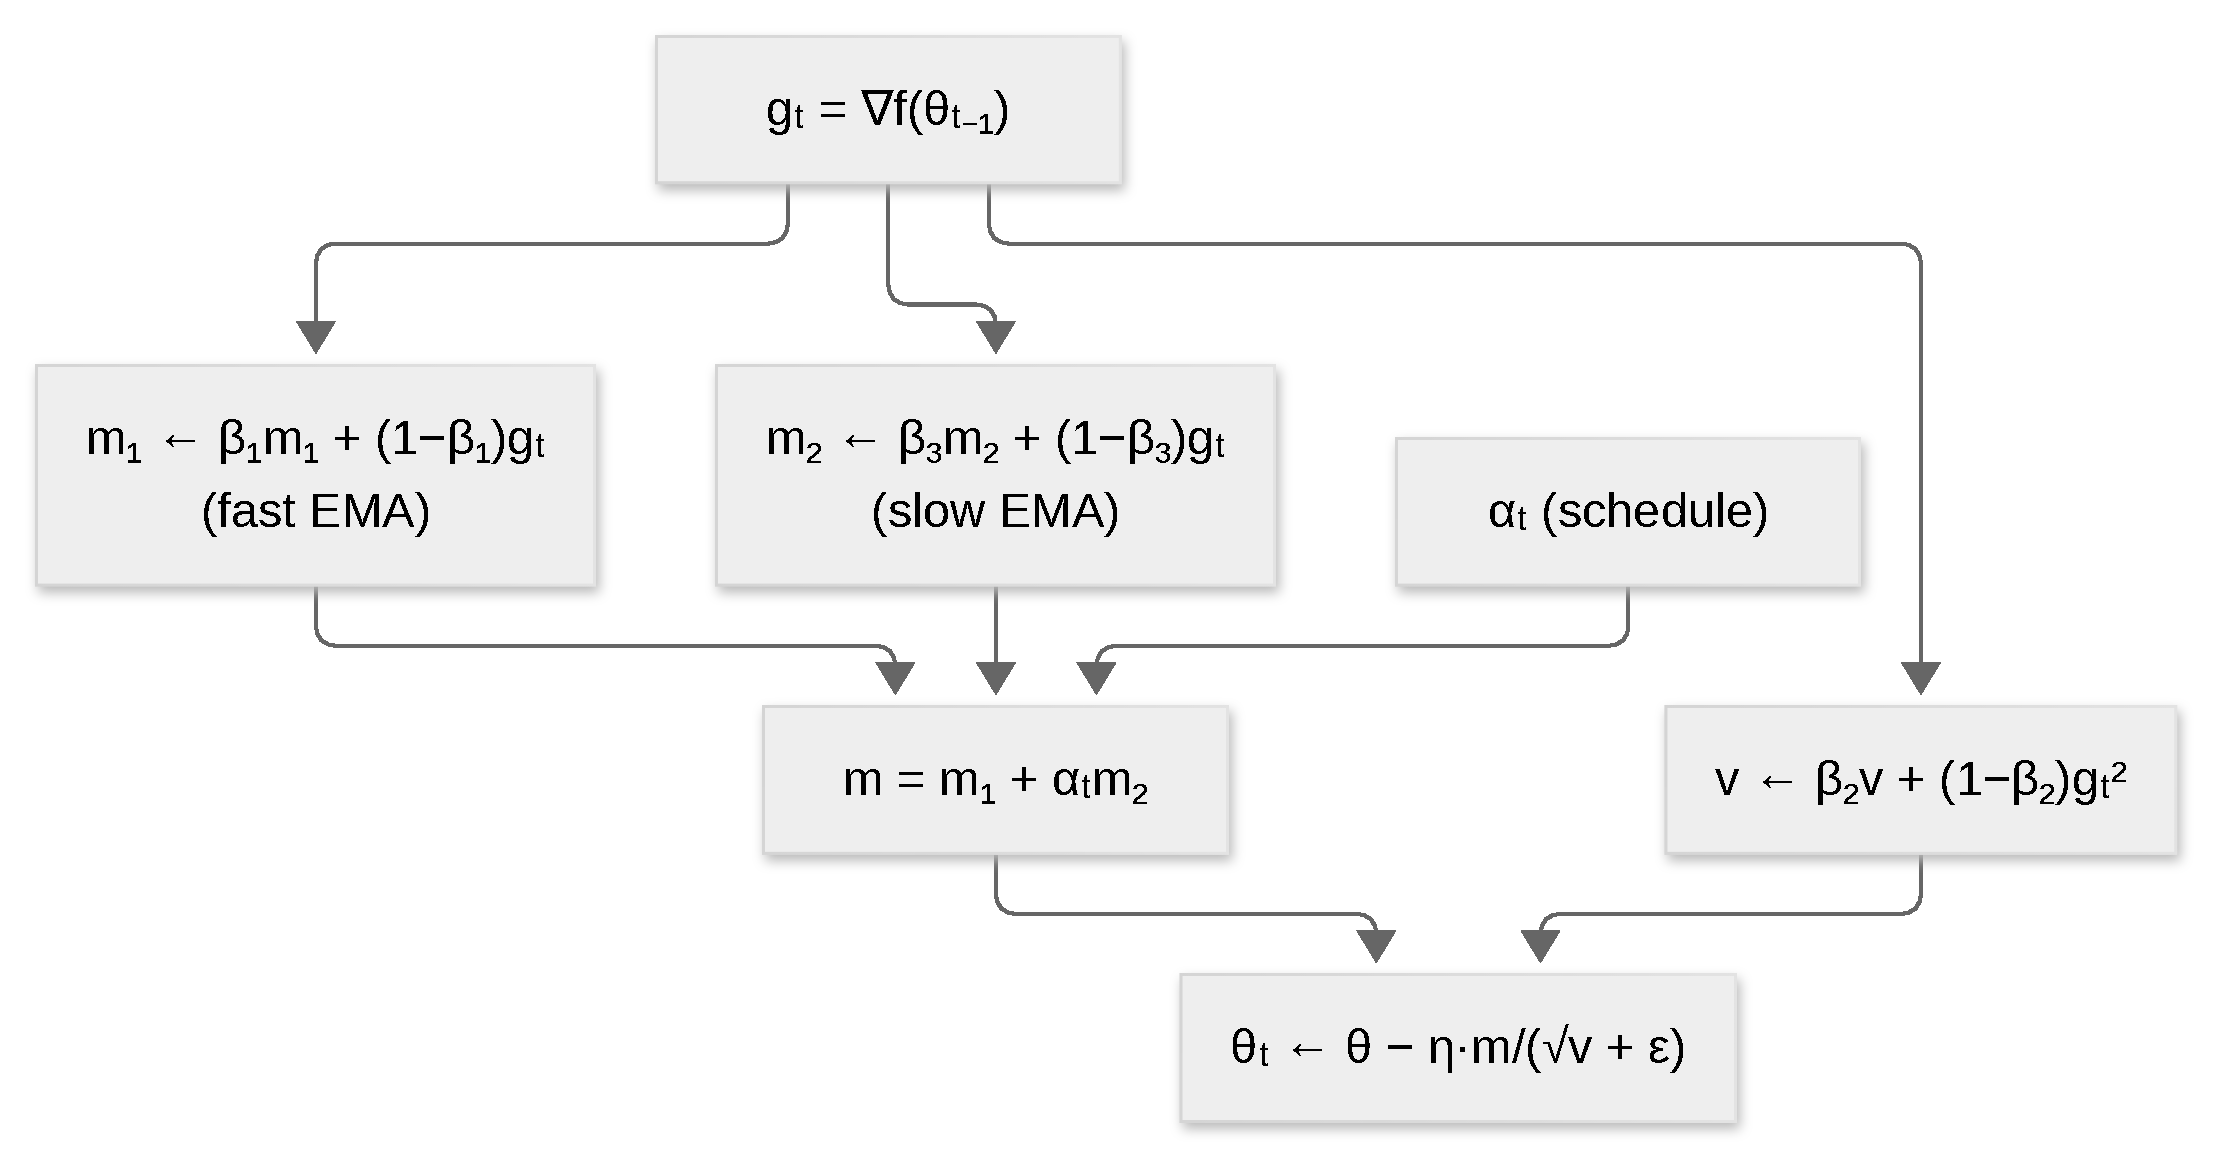
\includegraphics{figures/optimizers/ademamix.pdf}}
\caption{Step flow of AdEMAMix: parallel fast and slow gradient EMAs, mixed with a scheduled weight $\alpha_t$ before the adaptive update.}
\label{fig:opt-ademamix}
\end{figure}
AdEMAMix replaces Adam's single EMA of gradients with a \textbf{mixture of two EMAs}: one fast-decaying and one slow-decaying. This addresses the observation that gradients remain informative over tens of thousands of steps, not just hundreds:
\begin{align}
m_{1,t} &= \beta_1 m_{1,t-1} + (1-\beta_1)g_t \quad\text{(fast EMA, $\beta_1 \approx 0.9$)} \\
m_{2,t} &= \beta_3 m_{2,t-1} + (1-\beta_3)g_t \quad\text{(slow EMA, $\beta_3 \approx 0.9999$)} \\
v_t &= \beta_2 v_{t-1} + (1-\beta_2)g_t^2 \\
m_t &= m_{1,t} + \alpha_t m_{2,t} \quad\text{(mixture with scheduled weight $\alpha_t$)} \\
\theta_{t+1} &= \theta_t - \eta\frac{m_t}{\sqrt{v_t}+\epsilon}
\end{align}
The mixture weight $\alpha_t$ typically increases during training, allowing the fast EMA to provide immediate adaptation while the slow EMA accumulates long-range gradient correlations.

\begin{algorithm}[H]
\caption{AdEMAMix (Exponential Moving Average Mixture)}
\label{alg:ademamix}
\begin{algorithmic}[1]
\Require Initial parameters $\theta_0$, learning rate $\eta$, $\beta_1$ (fast), $\beta_3$ (slow), $\beta_2$ (second moment)
\Require Mixture weight $\alpha_t$ (typically increasing), tolerance $\epsilon$
\Ensure Updated parameters $\theta_T$
\State Initialize: $m_1 \gets 0$ (fast EMA), $m_2 \gets 0$ (slow EMA), $v \gets 0$
\For{$t = 1, 2, \ldots, T$}
    \State $g_t \gets \nabla f(\theta_{t-1})$
    \If{weight\_decay $> 0$}
        \State $\theta_{t-1} \gets \theta_{t-1}(1 - \eta\lambda)$
    \EndIf
    \State $m_1 \gets \beta_1 m_1 + (1-\beta_1) g_t$ \Comment{Fast EMA}
    \State $m_2 \gets \beta_3 m_2 + (1-\beta_3) g_t$ \Comment{Slow EMA}
    \State $v \gets \beta_2 v + (1-\beta_2) g_t^2$
    \State $m_t \gets m_1 + \alpha_t m_2$ \Comment{Mixture}
    \State $\theta_t \gets \theta_{t-1} - \eta (m_t / (\sqrt{v} + \epsilon))$
\EndFor
\Return $\theta_T$
\end{algorithmic}
\end{algorithm}

\paragraph{Cons.}
\begin{itemize}[leftmargin=*]
\item Two gradient EMAs plus the second moment roughly triple Adam's optimizer state.
\item The mixture schedule $\alpha_t$ adds a hyperparameter to tune.
\end{itemize}

\paragraph{Pros.}
\begin{itemize}[leftmargin=*]
\item Exploits gradient information that remains informative over tens of thousands of steps.
\item A 1.3B model on 101B tokens matches AdamW on 197B tokens (95\% data-efficiency gain), suggesting reduced forgetting.
\end{itemize}

\paragraph{MARS (Make Adaptive learning Rates Shine).}
\begin{figure}[H]
\centering
\fitfigure{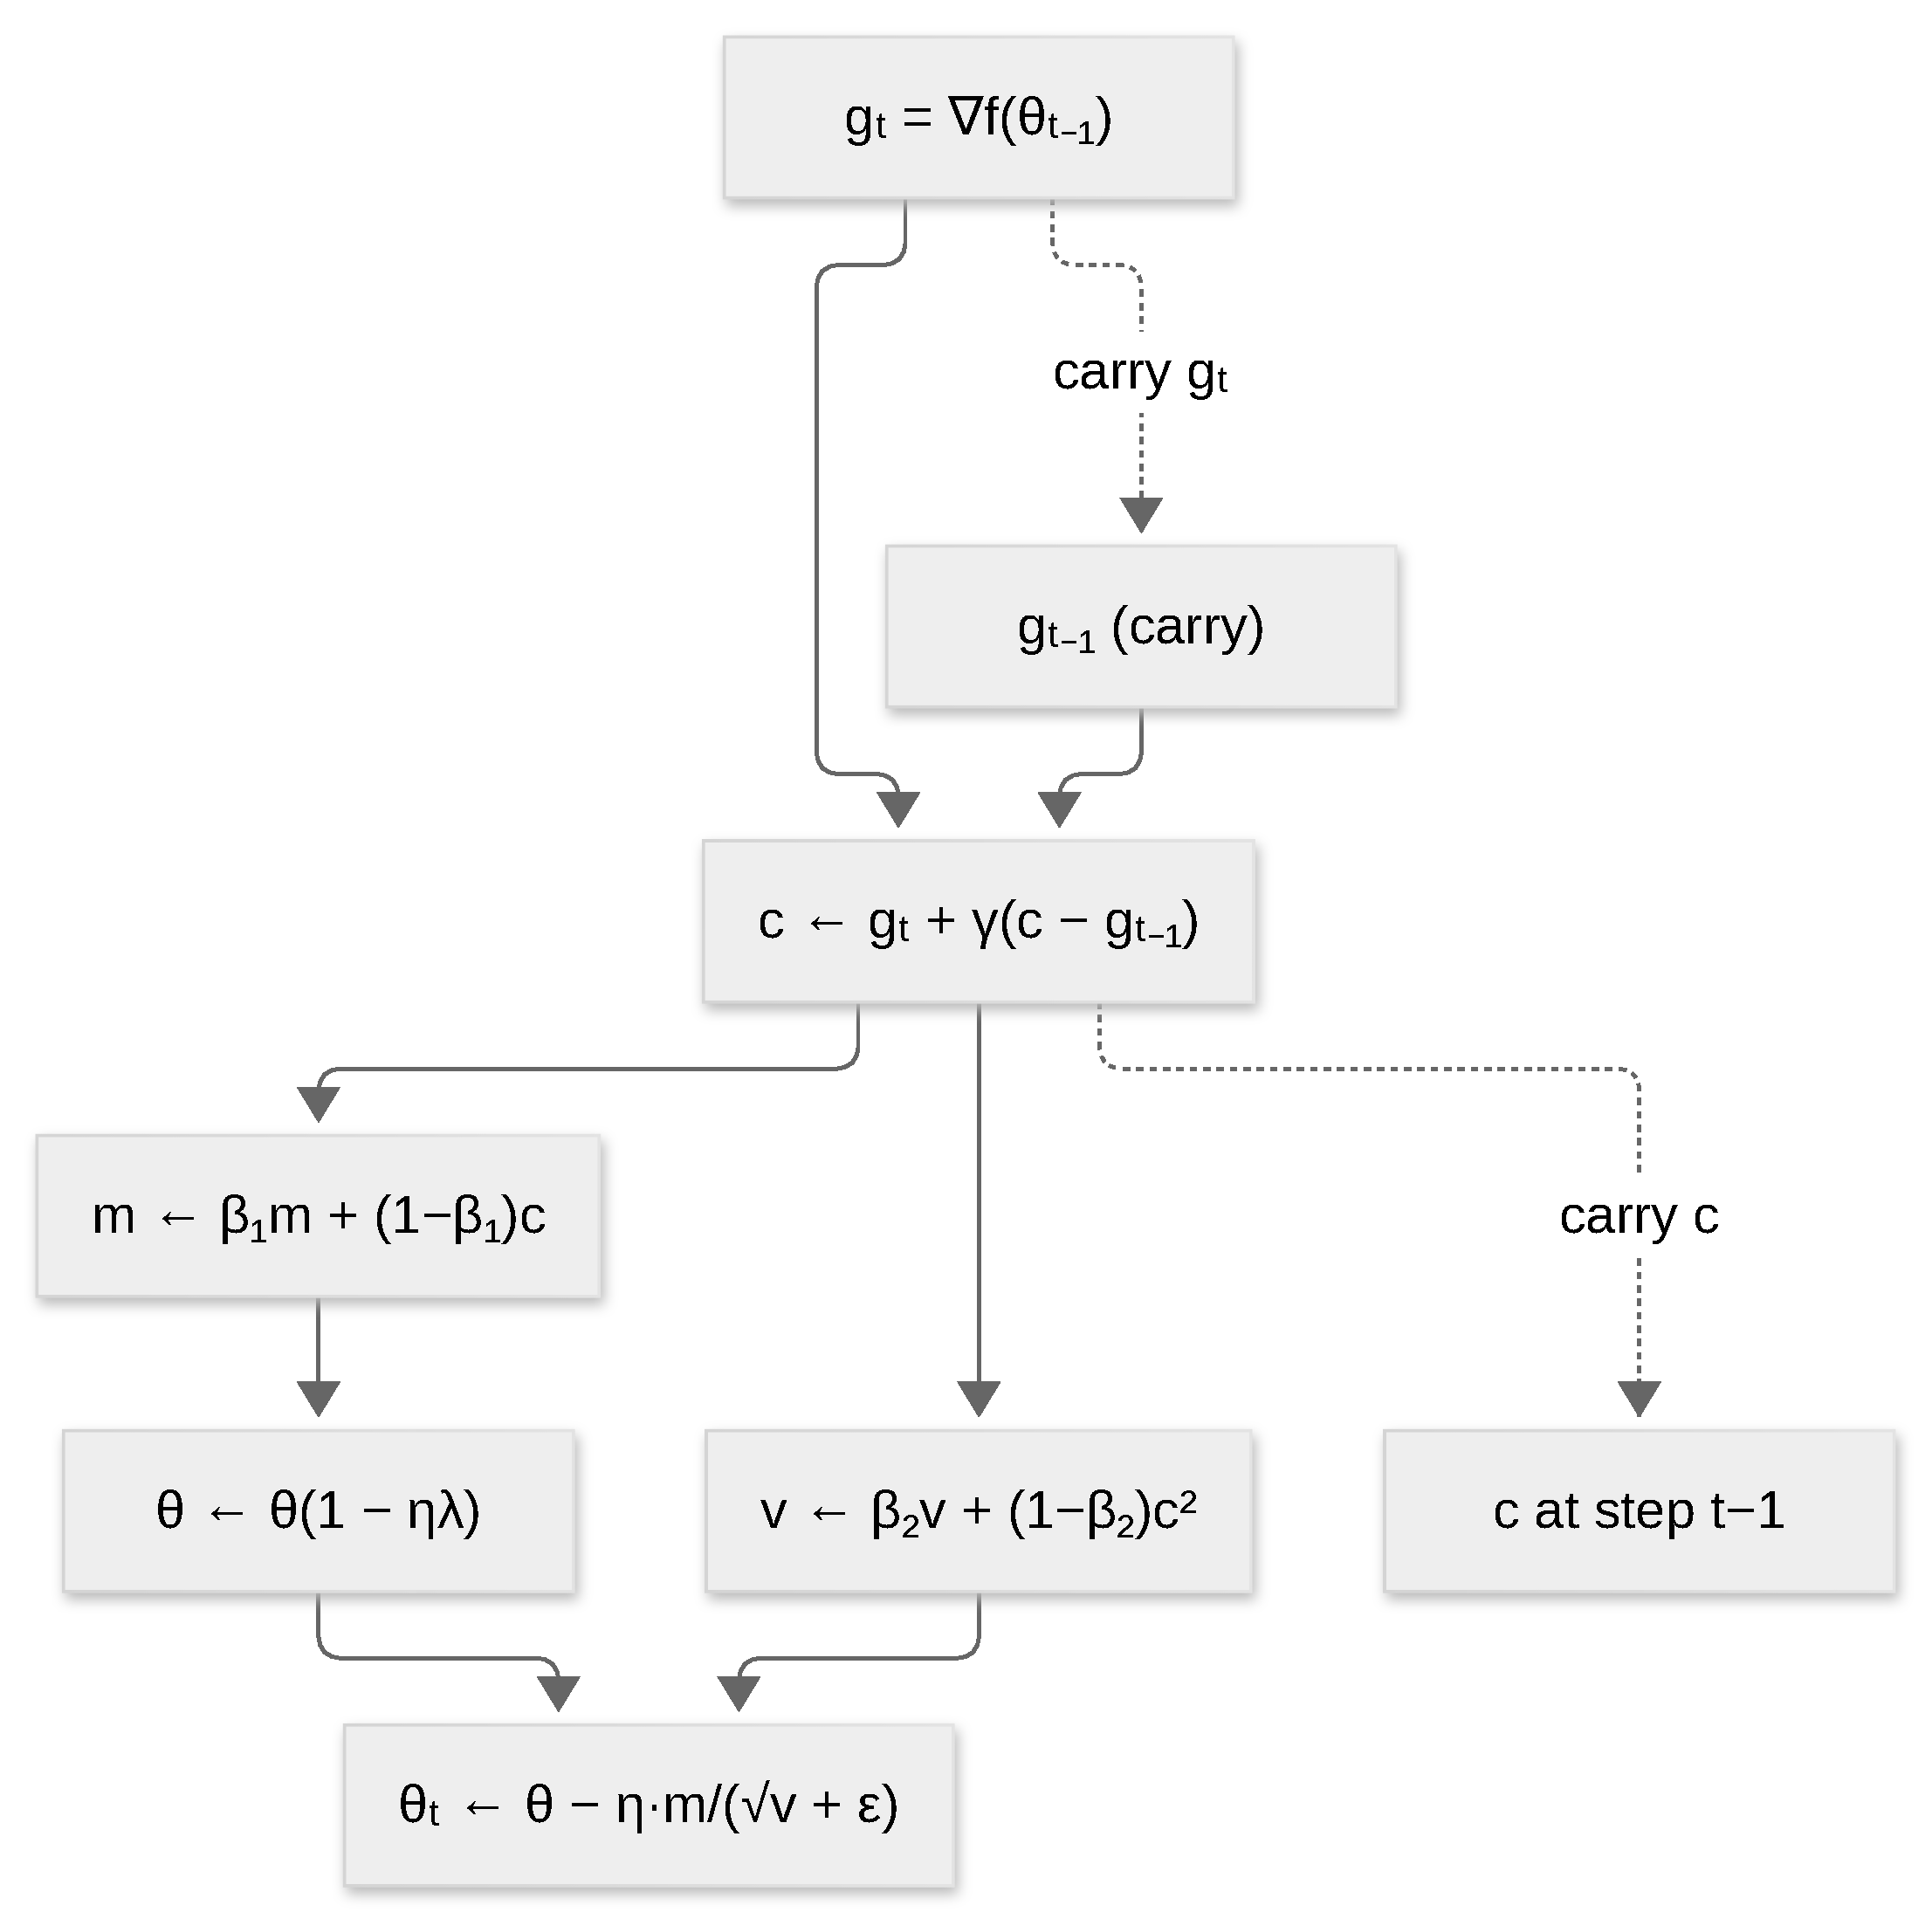
\includegraphics{figures/optimizers/mars.pdf}}
\caption{Step flow of MARS: a recursive variance-reduced gradient estimate feeding Adam-style first and second moments.}
\label{fig:opt-mars}
\end{figure}
MARS combines preconditioned gradient methods (e.g., AdamW) with \textbf{variance reduction} via scaled stochastic recursive momentum. The core innovation is a variance-reduced gradient estimate:
\begin{align}
c_t &= g_t + \gamma(c_{t-1} - g_{t-1}) \quad\text{(SVRG-style recursive estimate)} \\
m_t &= \beta_1 m_{t-1} + (1-\beta_1)c_t \\
v_t &= \beta_2 v_{t-1} + (1-\beta_2)c_t^2 \\
\theta_{t+1} &= \theta_t - \eta\frac{m_t}{\sqrt{v_t}+\epsilon}
\end{align}
where $\gamma \in [0.01, 0.1]$ controls how much historical gradient information is retained. The variance-reduced gradient $c_t$ acts as an implicit noise filter, amplifying consistent signal directions and dampening contradictory noise.

\begin{algorithm}[H]
\caption{MARS (Make Adaptive learning Rates Shine)}
\label{alg:mars}
\begin{algorithmic}[1]
\Require Initial parameters $\theta_0$, learning rate $\eta$, $\beta_1, \beta_2$, weight decay $\lambda$
\Require Variance reduction coefficient $\gamma \in [0.01, 0.1]$
\Ensure Updated parameters $\theta_T$
\State Initialize: $m \gets 0$, $v \gets 0$, $c \gets 0$ (variance-reduced gradient), $g_{-1} \gets 0$
\For{$t = 1, 2, \ldots, T$}
    \State $g_t \gets \nabla f(\theta_{t-1})$
    \State Variance reduction: $c \gets g_t + \gamma(c - g_{t-1})$
    \State $m \gets \beta_1 m + (1-\beta_1) c$
    \State $v \gets \beta_2 v + (1-\beta_2) c^2$
    \If{weight\_decay $> 0$}
        \State $\theta_{t-1} \gets \theta_{t-1}(1 - \eta\lambda)$
    \EndIf
    \State $\theta_t \gets \theta_{t-1} - \eta (m / (\sqrt{v} + \epsilon))$
    \State $g_{t-1} \gets g_t$
\EndFor
\Return $\theta_T$
\end{algorithmic}
\end{algorithm}

\paragraph{Cons.}
\begin{itemize}[leftmargin=*]
\item Stores the variance-reduced gradient and the previous gradient in addition to Adam's moments.
\item The variance-reduction coefficient $\gamma \in [0.01, 0.1]$ must be tuned.
\end{itemize}

\paragraph{Pros.}
\begin{itemize}[leftmargin=*]
\item Acts as an implicit noise filter, amplifying consistent directions and dampening contradictory noise.
\item MARS-AdamW consistently outperforms bare AdamW by significant margins on GPT-2 pretraining.
\end{itemize}

\paragraph{Cautious Optimizers (Cautious AdamW, Cautious Lion).}
\begin{figure}[H]
\centering
\fitfigure{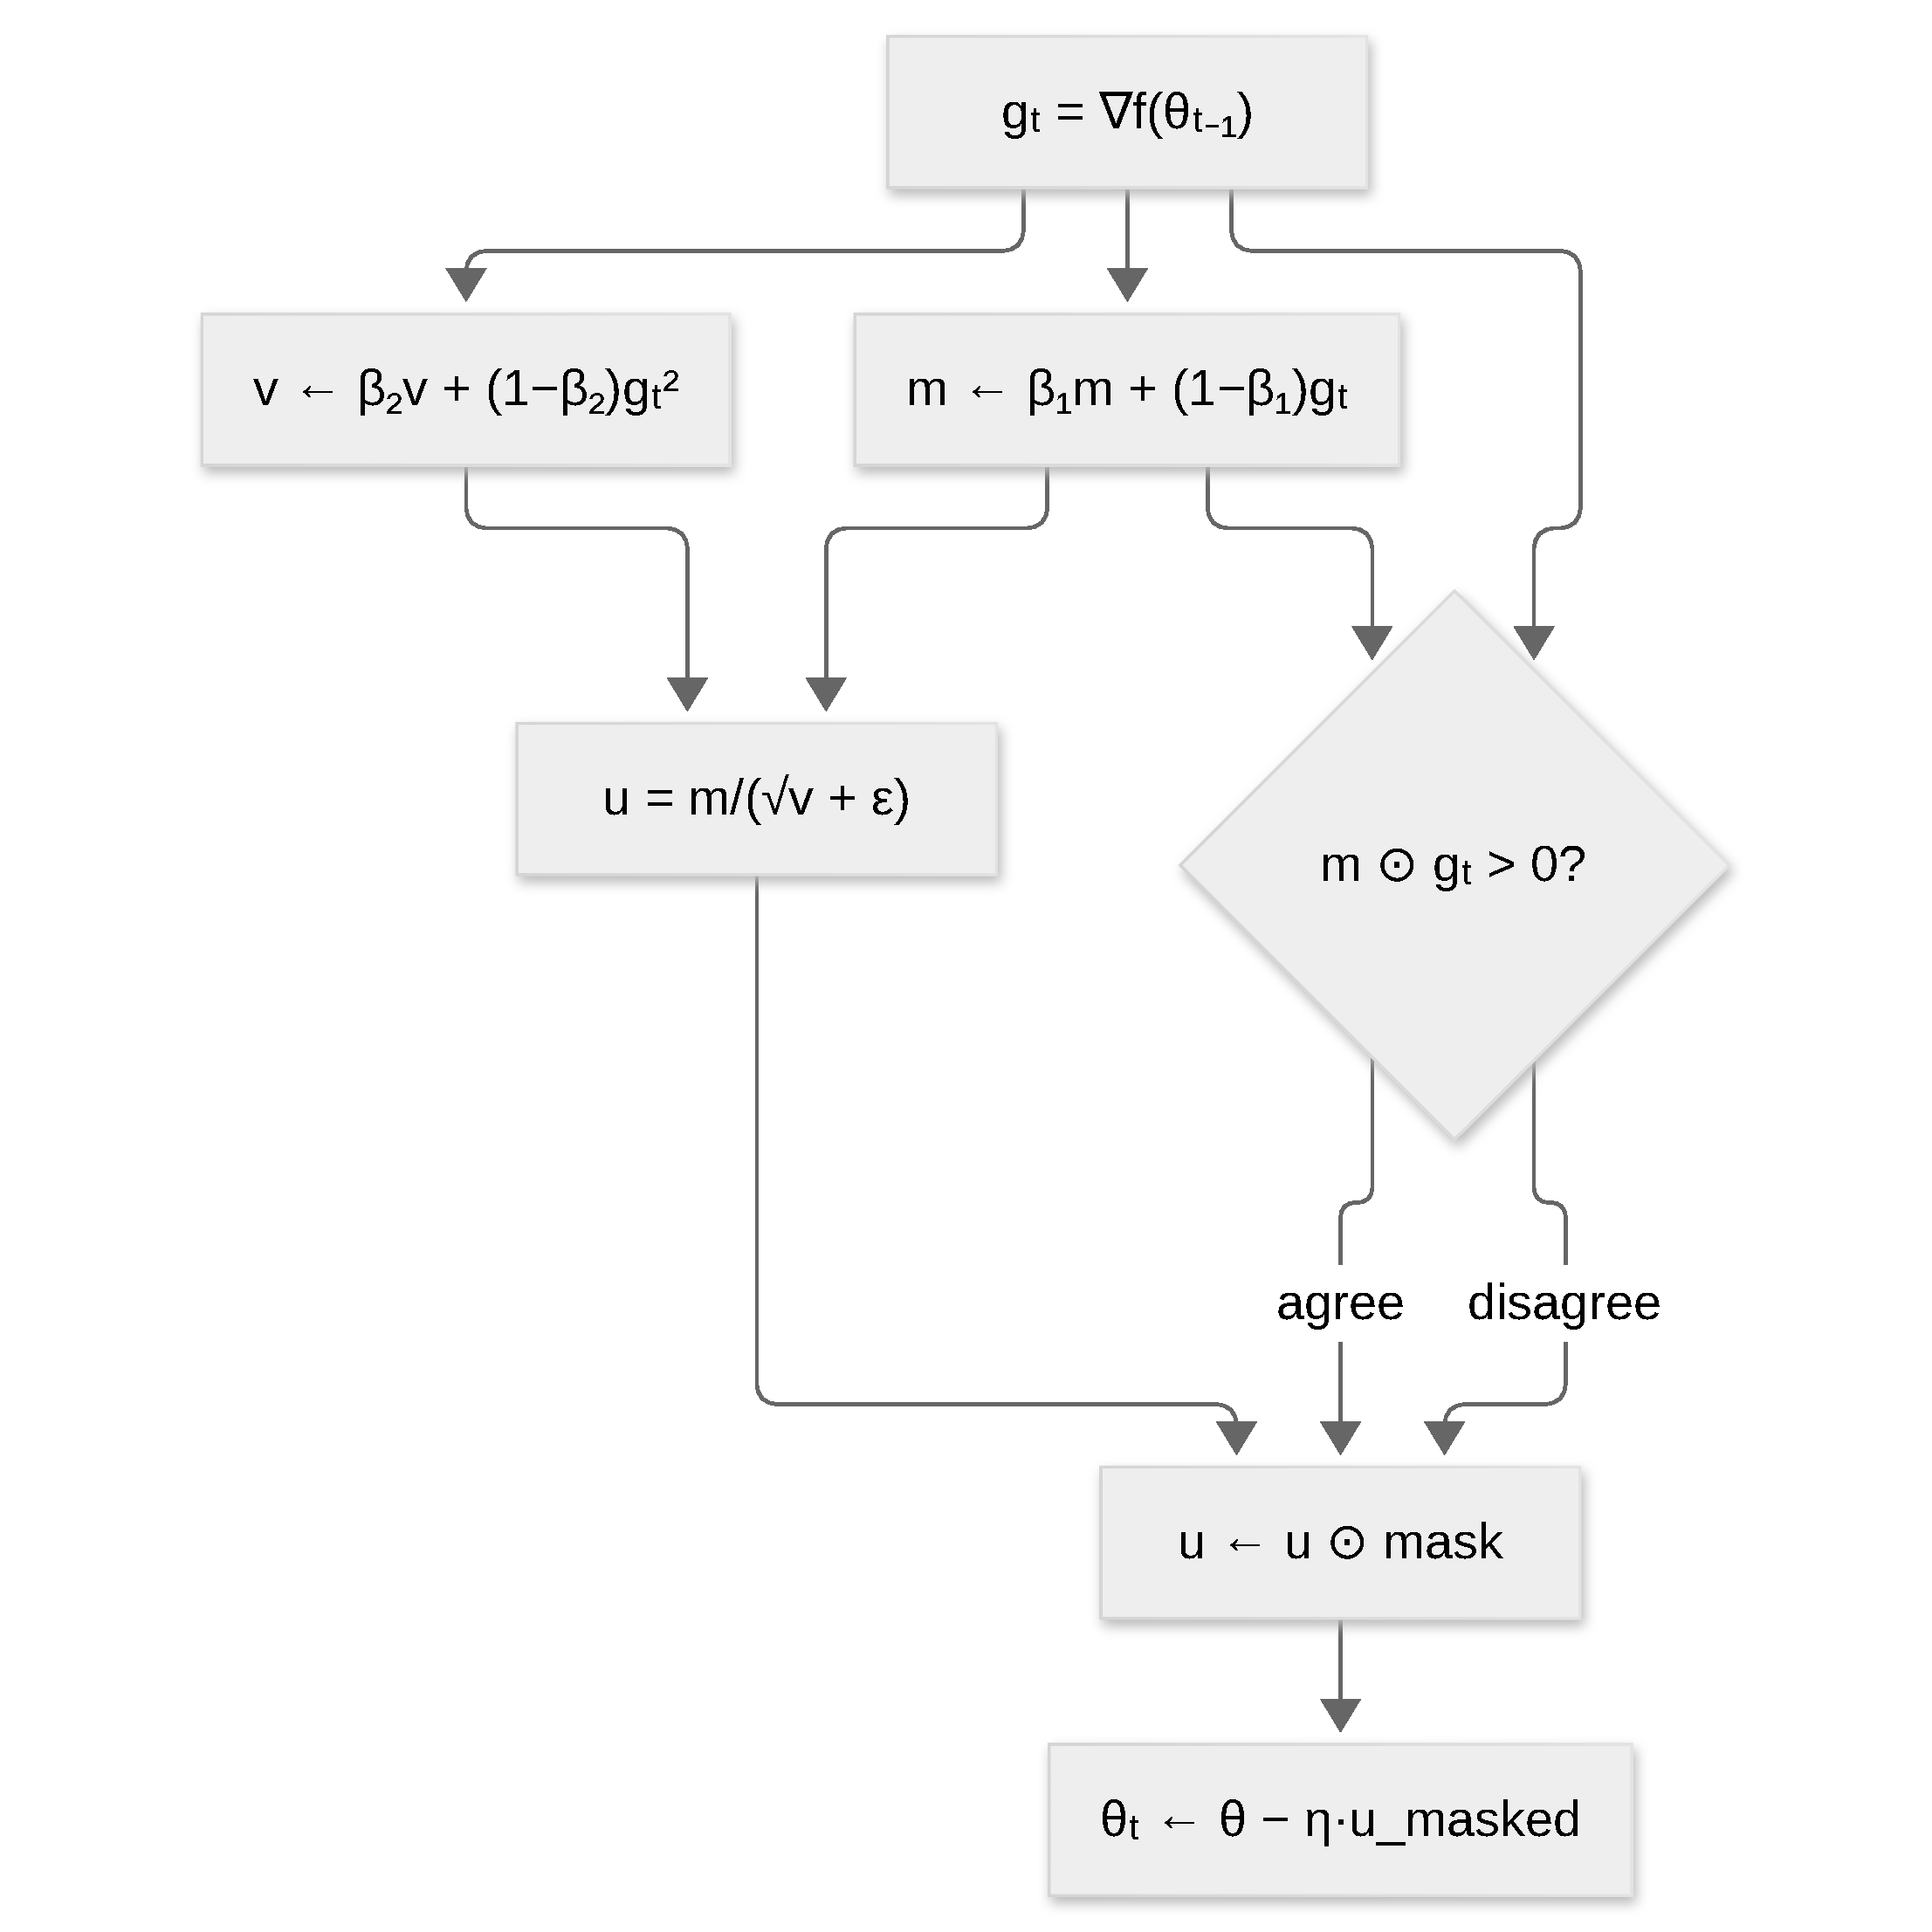
\includegraphics{figures/optimizers/cautious.pdf}}
\caption{Step flow of Cautious AdamW: a consensus mask keeps only update coordinates where momentum and gradient agree.}
\label{fig:opt-cautious}
\end{figure}
The Cautious framework applies a \textbf{one-line modification} to any momentum-based optimizer: mask the update so that only dimensions where momentum and gradient directions agree are applied:
\begin{align}
\text{mask}_i &= \begin{cases} 1 & \text{if } m_t[i] \cdot g_t[i] > 0 \quad\text{(agreement)} \\ 0 & \text{otherwise} \end{cases} \\
u_t &= \left(\frac{m_t}{\sqrt{v_t}+\epsilon}\right) \odot \text{mask} \quad\text{(element-wise masking)} \\
\theta_{t+1} &= \theta_t - \eta u_t
\end{align}
The intuition: momentum $m_t$ estimates the gradient direction from history; the current gradient $g_t$ is instantaneous signal. When both agree, the optimizer is confident and should update aggressively. When they disagree, the optimizer is conflicted---the historical trend points toward a region that may have been good before, but current evidence contradicts it. By masking conflicted dimensions, Cautious becomes more conservative and avoids corrupted steps.

\begin{algorithm}[H]
\caption{Cautious AdamW (Consensus-based Update Masking)}
\label{alg:cautious}
\begin{algorithmic}[1]
\Require Initial parameters $\theta_0$, learning rate $\eta$, $\beta_1, \beta_2$, weight decay $\lambda$
\Ensure Updated parameters $\theta_T$
\State Initialize: $m \gets 0$, $v \gets 0$
\For{$t = 1, 2, \ldots, T$}
    \State $g_t \gets \nabla f(\theta_{t-1})$
    \State $m \gets \beta_1 m + (1-\beta_1) g_t$
    \State $v \gets \beta_2 v + (1-\beta_2) g_t^2$
    \State Consensus mask: $\text{mask}_i \gets 1$ if $m[i] \cdot g_t[i] > 0$, else $0$ \Comment{Agreement}
    \State Base Adam update: $u \gets m / (\sqrt{v} + \epsilon)$
    \State Apply mask: $u_{\text{masked}} \gets u \odot \text{mask}$ \Comment{Element-wise}
    \If{weight\_decay $> 0$}
        \State $\theta_{t-1} \gets \theta_{t-1}(1 - \eta\lambda)$
    \EndIf
    \State $\theta_t \gets \theta_{t-1} - \eta u_{\text{masked}}$
\EndFor
\Return $\theta_T$
\end{algorithmic}
\end{algorithm}

\paragraph{Cons.}
\begin{itemize}[leftmargin=*]
\item Masking can discard useful updates when momentum and gradient temporarily disagree.
\item Requires a base momentum optimizer plus the element-wise mask.
\end{itemize}

\paragraph{Pros.}
\begin{itemize}[leftmargin=*]
\item A one-line modification applicable to any momentum-based optimizer.
\item Up to \textbf{1.47$\times$ speedup} on Llama and MAE pretraining while preserving convergence guarantees.
\end{itemize}

\subsection{Large-Batch, Memory-Efficient, and Parameter-Free Optimizers}
\paragraph{LAMB (Layer-wise Adaptive Moments optimizer for Batch training).}
\begin{figure}[H]
\centering
\fitfigure{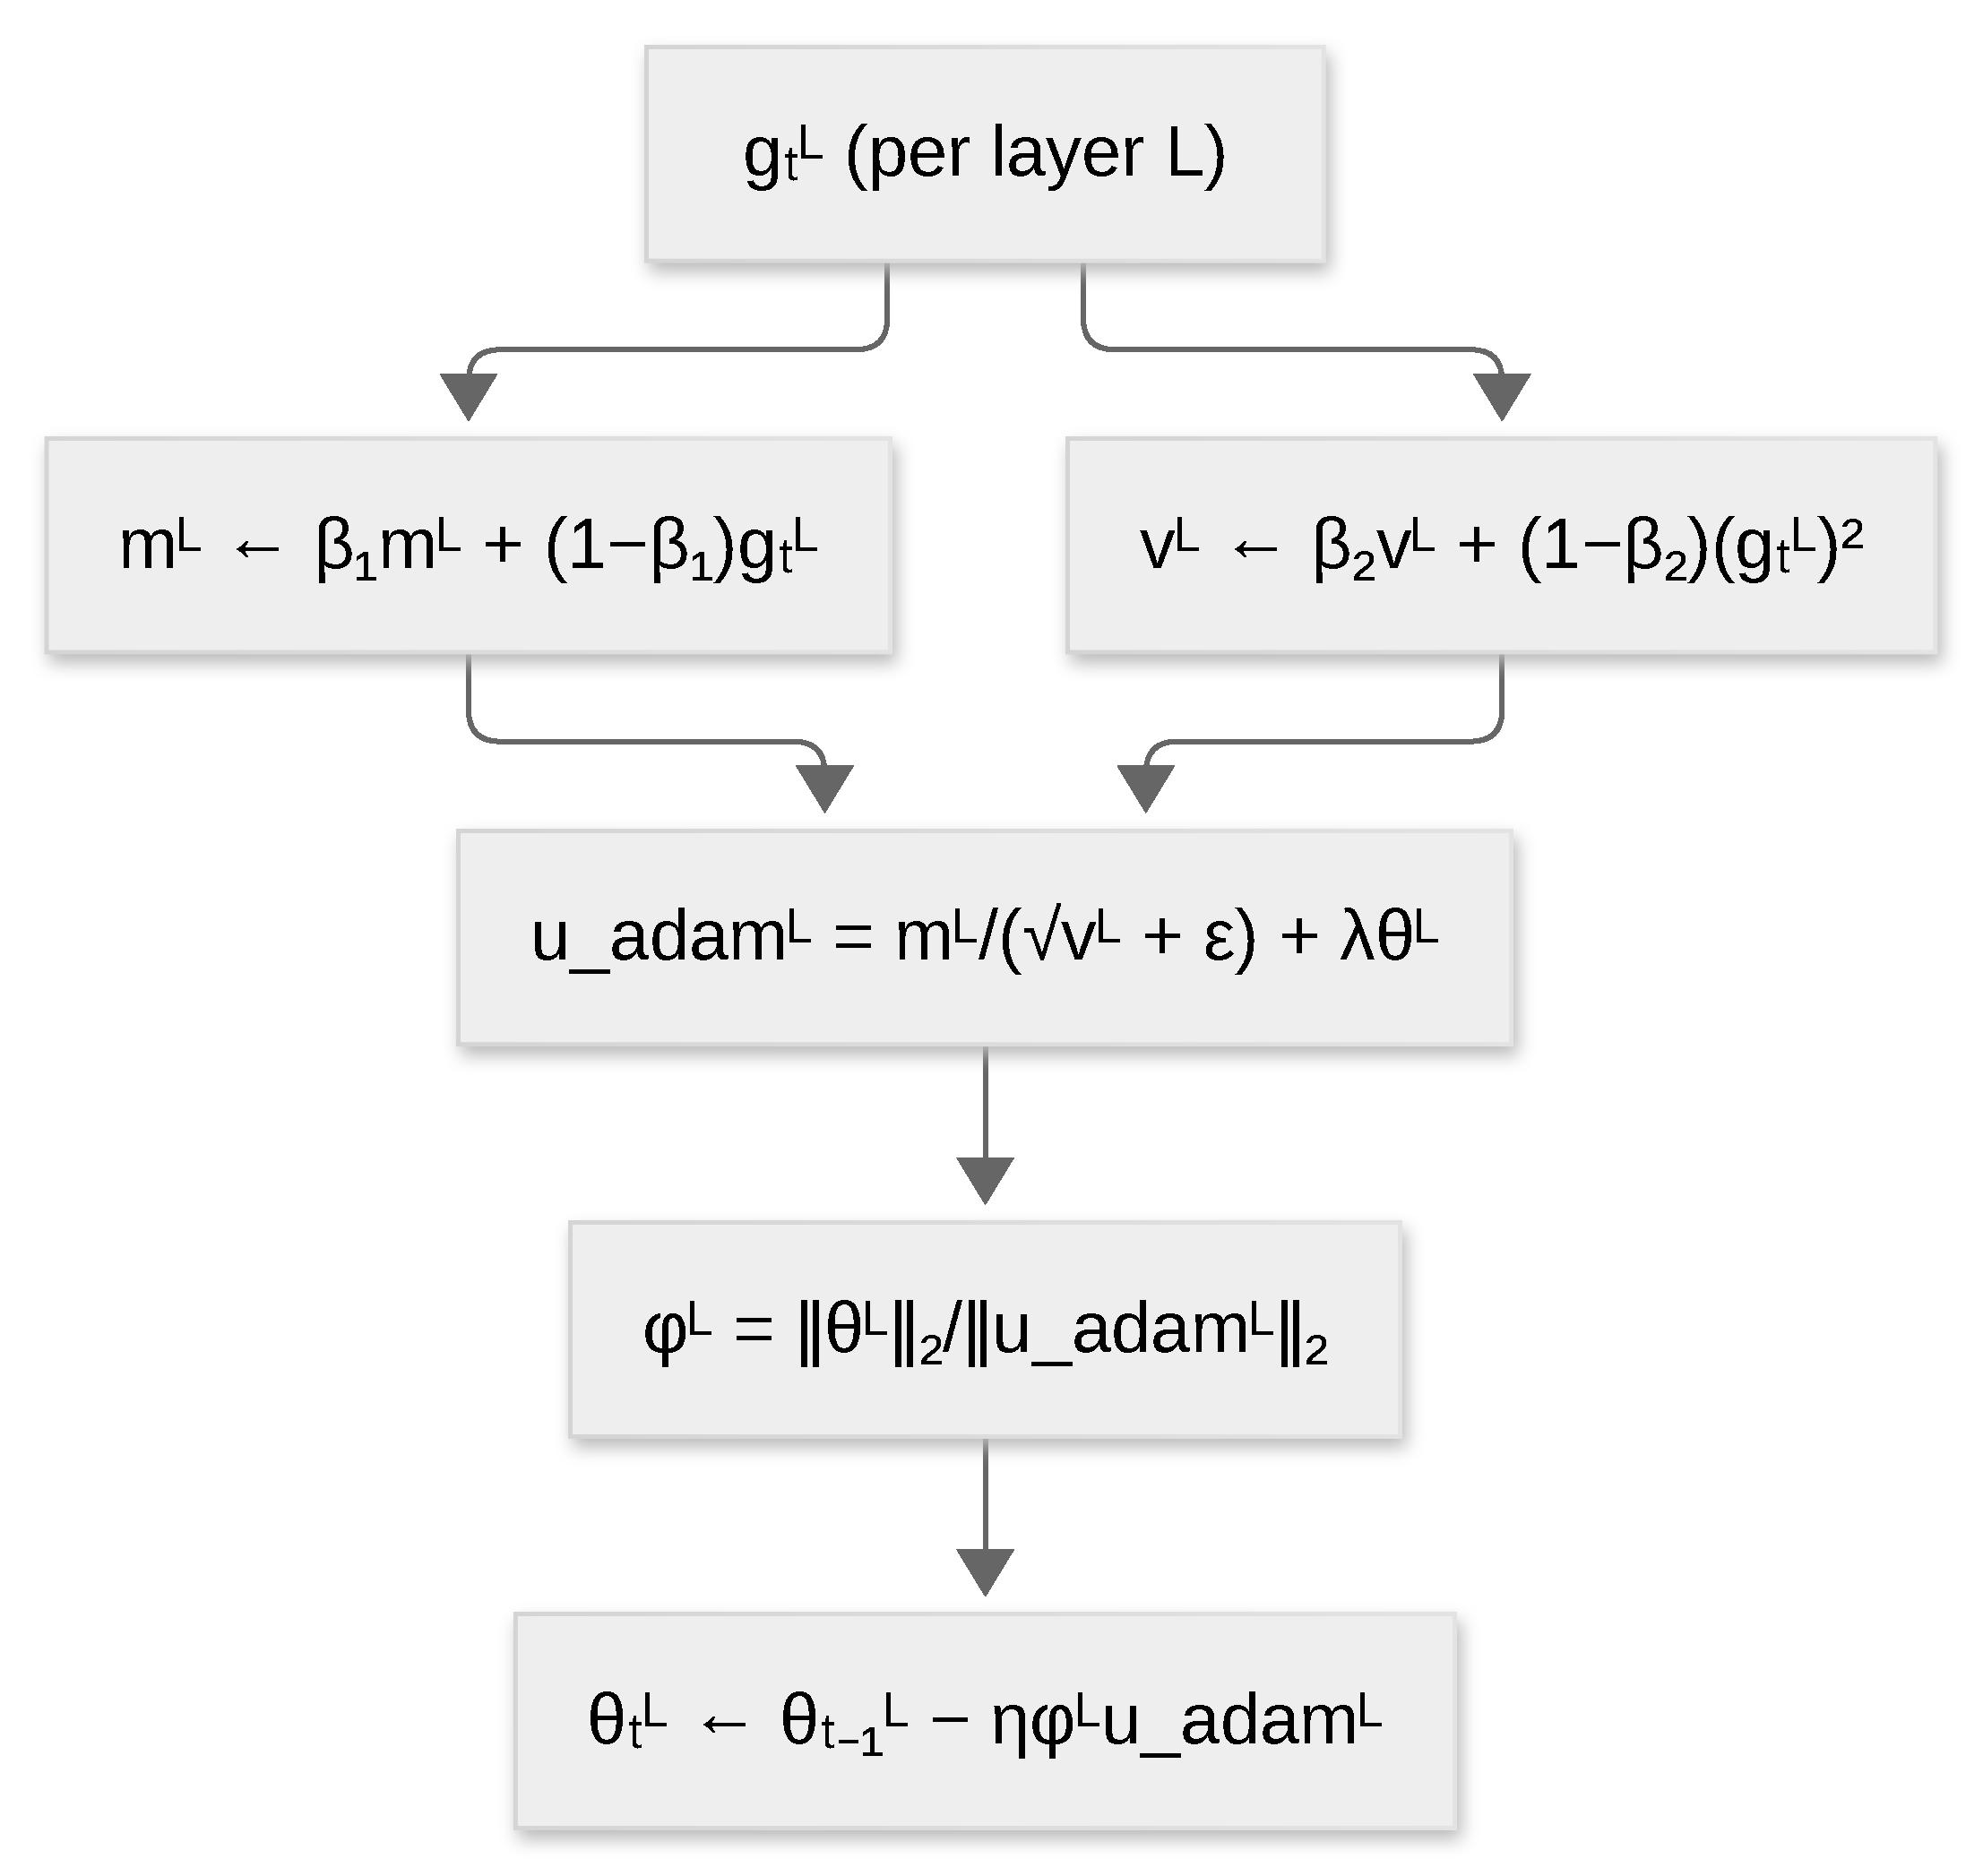
\includegraphics{figures/optimizers/lamb.pdf}}
\caption{Step flow of LAMB: per-layer Adam step rescaled by the trust ratio between weight and update norms.}
\label{fig:opt-lamb}
\end{figure}
LAMB extends Adam with \textbf{layer-wise adaptive rate scaling} (inspired by LARS), enabling stable training with extreme batch sizes (e.g., 64K on BERT):
\begin{align}
m_t^L &= \beta_1 m_{t-1}^L + (1-\beta_1)g_t^L \quad\text{(layer-wise first moment)} \\
v_t^L &= \beta_2 v_{t-1}^L + (1-\beta_2)(g_t^L)^2 \\
u_{\text{adam}}^L &= \frac{m_t^L}{\sqrt{v_t^L}+\epsilon} + \lambda\theta_{t-1}^L \quad\text{(base adaptive step with decay)} \\
\phi^L &= \frac{\|\theta_{t-1}^L\|_2}{\|u_{\text{adam}}^L\|_2} \quad\text{(trust ratio: layer normalization)} \\
\theta_t^L &= \theta_{t-1}^L - \eta \cdot \phi^L \cdot u_{\text{adam}}^L
\end{align}
The \textbf{trust ratio} $\phi^L = \|\theta^L\|_2 / \|u_{\text{adam}}^L\|_2$ normalizes the effective update step relative to weight magnitude. In very large batches, stochastic gradient noise can exceed signal, destabilizing layer-wise learning rates. By scaling updates proportionally to weight norms, LAMB ensures relative changes rather than absolute ones, preventing small confident updates in large vectors from dominating.

\begin{algorithm}[H]
\caption{LAMB (Layer-wise Adaptive Moments optimizer for Batch training)}
\label{alg:lamb}
\begin{algorithmic}[1]
\Require Initial parameters $\theta_0$, learning rate $\eta$, $\beta_1, \beta_2$, weight decay $\lambda$
\Ensure Updated parameters $\theta_T$
\State Initialize: For each layer $L$: $m^L \gets 0$, $v^L \gets 0$
\For{$t = 1, 2, \ldots, T$}
    \For{each layer $L$}
        \State $g_t^L \gets \nabla f(\theta_t^L)$
        \State $m^L \gets \beta_1 m^L + (1-\beta_1) g_t^L$
        \State $v^L \gets \beta_2 v^L + (1-\beta_2) (g_t^L)^2$
        \State Base Adam: $u_{\text{adam}}^L \gets m^L / (\sqrt{v^L} + \epsilon)$
        \If{weight\_decay $> 0$}
            \State $u_{\text{adam}}^L \gets u_{\text{adam}}^L + \lambda \theta_{t-1}^L$
        \EndIf
        \State Trust ratio: $\phi^L \gets \|\theta_{t-1}^L\|_2 / \|u_{\text{adam}}^L\|_2$ if both nonzero, else $1$
        \State $\theta_t^L \gets \theta_{t-1}^L - \eta \phi^L u_{\text{adam}}^L$
    \EndFor
\EndFor
\Return $\theta_T$
\end{algorithmic}
\end{algorithm}

\paragraph{Cons.}
\begin{itemize}[leftmargin=*]
\item Layer-wise norm bookkeeping and trust-ratio computation add per-step overhead.
\item The trust ratio is unstable when layer or update norms are close to zero.
\end{itemize}

\paragraph{Pros.}
\begin{itemize}[leftmargin=*]
\item Enables stable training with extreme batch sizes (e.g., 64K on BERT).
\item Preserves small-batch generalization benefits while scaling the batch.
\end{itemize}

\paragraph{Schedule-Free AdamW.}
\begin{figure}[H]
\centering
\fitfigure{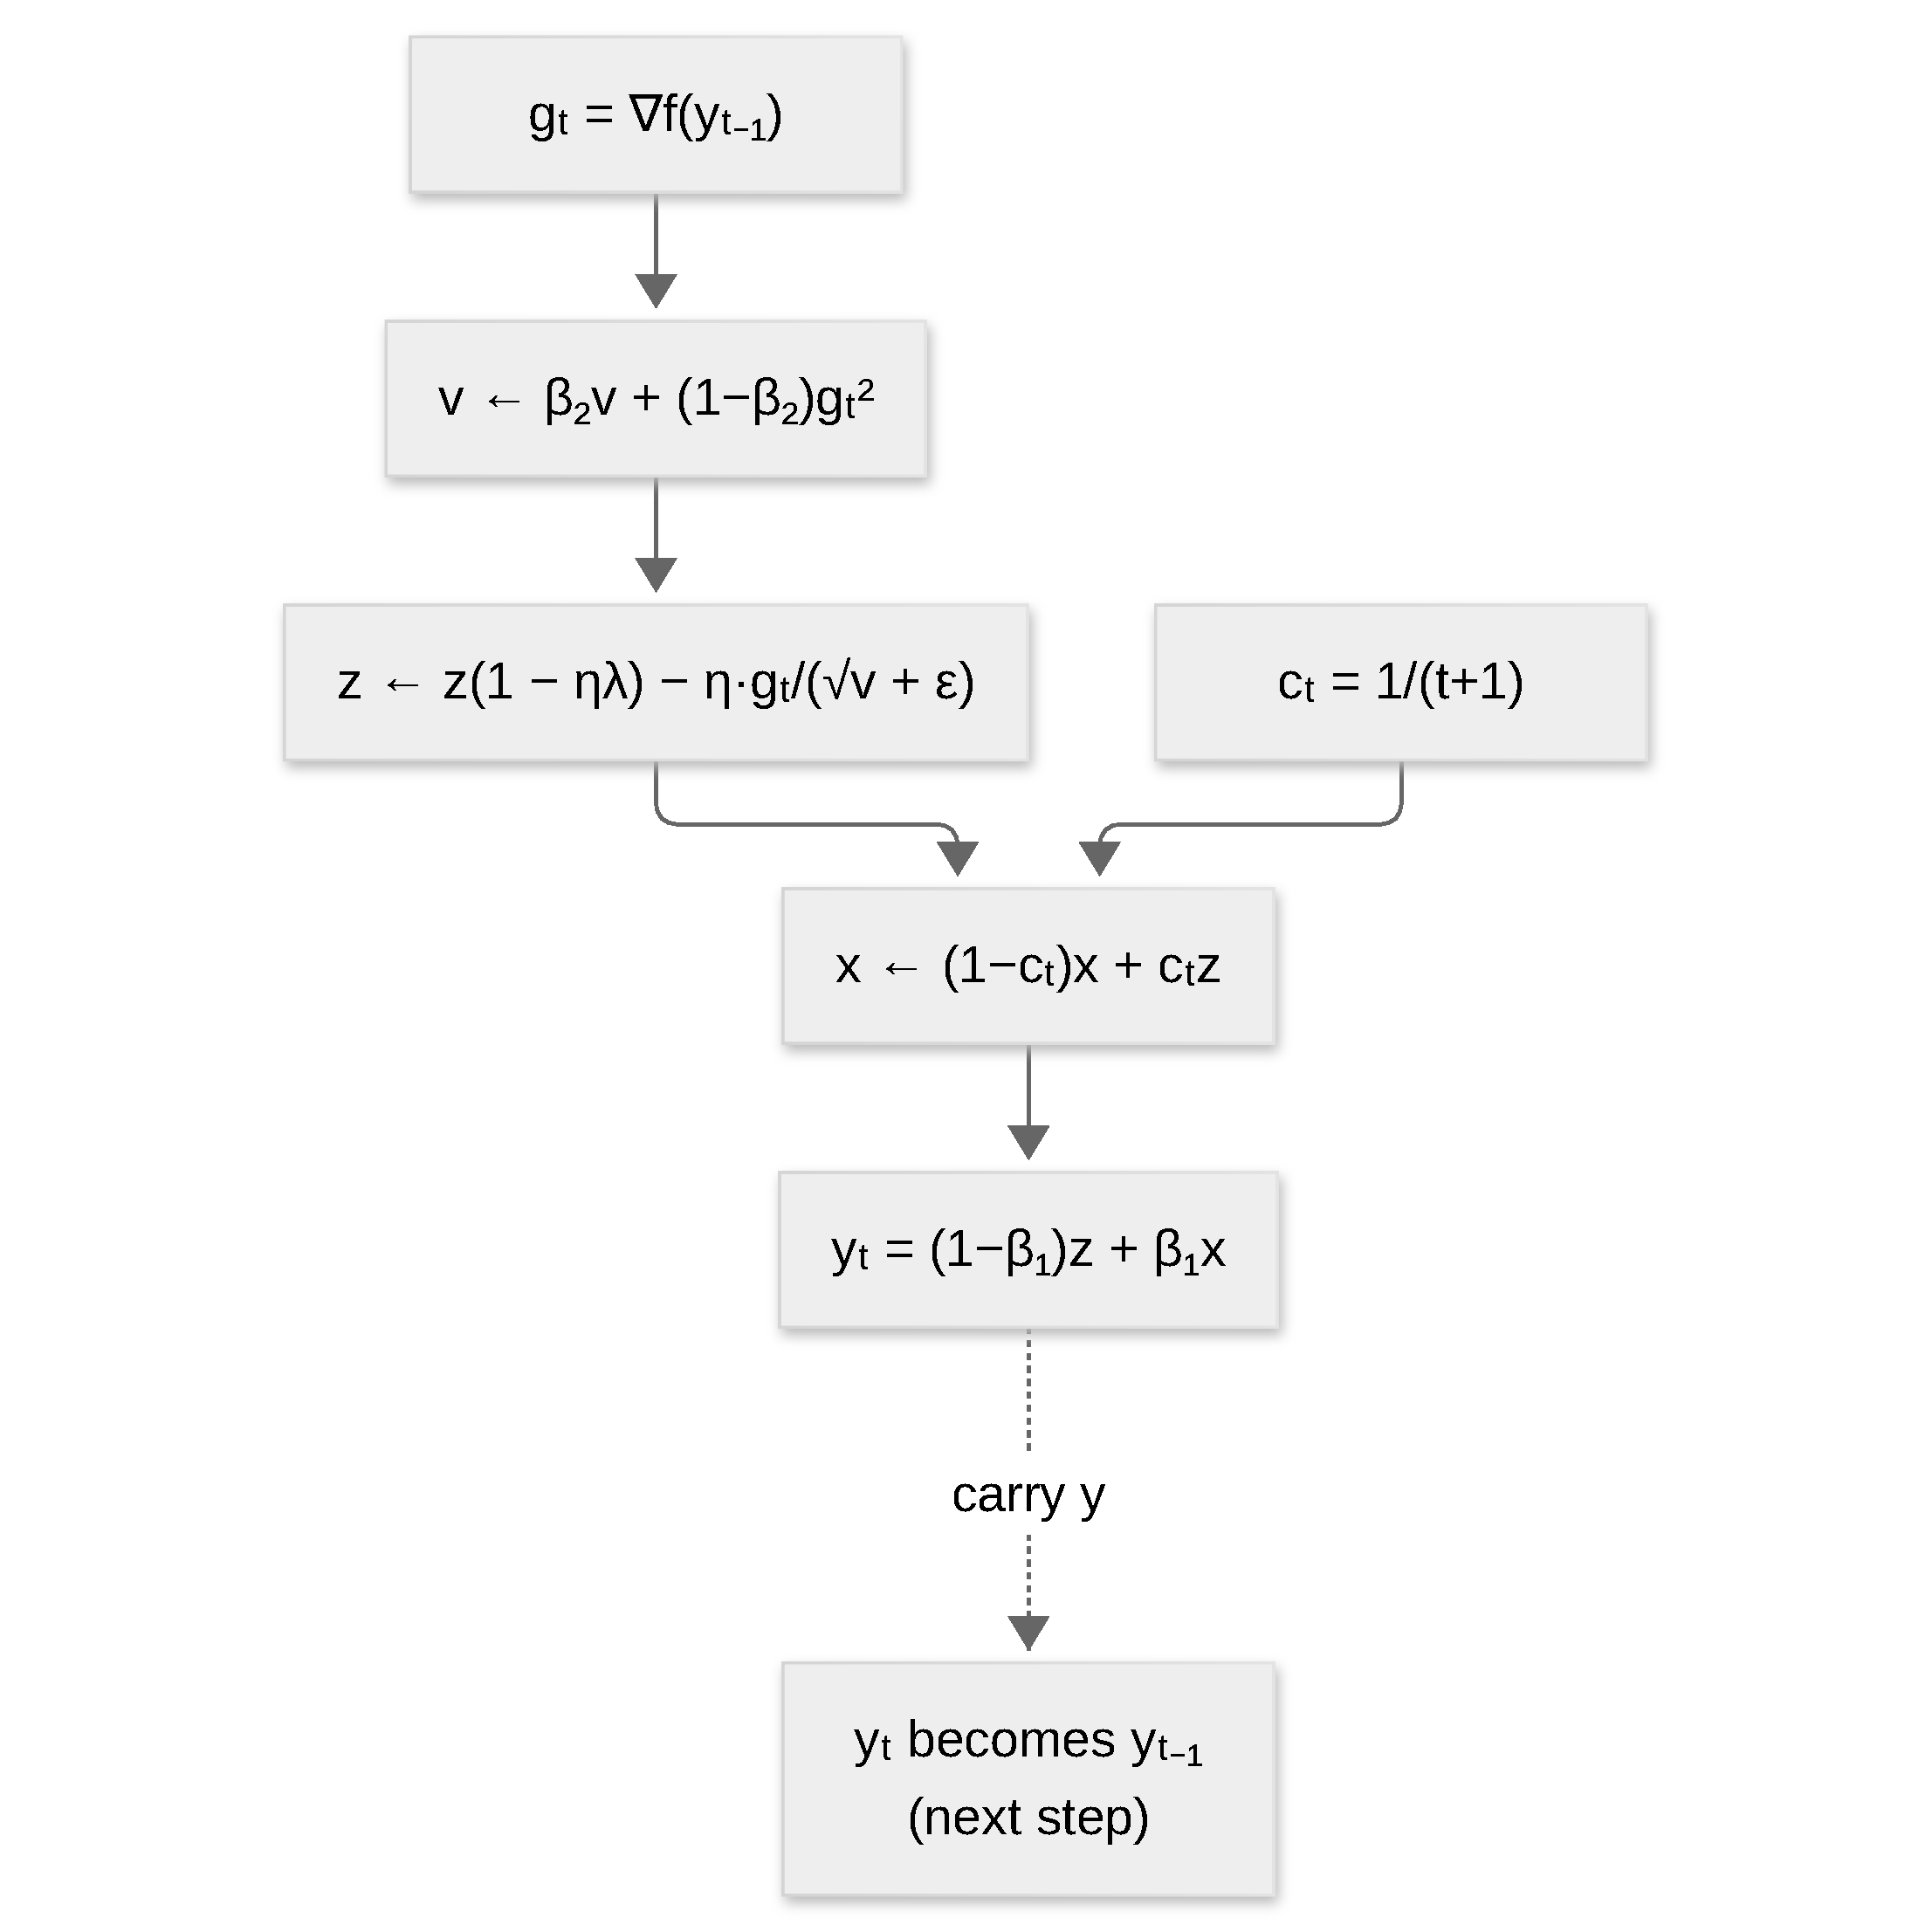
\includegraphics{figures/optimizers/schedulefree.pdf}}
\caption{Step flow of Schedule-Free AdamW: exploration stream $z$, iterate average $x$, and interpolation point $y$, with implicit $1/(t+1)$ averaging.}
\label{fig:opt-schedulefree}
\end{figure}
Schedule-free methods remove explicit scheduler design from the optimization recipe. The algorithm maintains two parameter streams: $z_t$ (exploration) and $x_t$ (smooth average):
\begin{align}
v_t &= \beta_2 v_{t-1} + (1-\beta_2)g_t^2 \quad\text{(variance)} \\
z_t &= z_{t-1}(1-\eta\lambda) - \eta\frac{g_t}{\sqrt{v_t}+\epsilon} \quad\text{(adaptive step with decay)} \\
c_t &= \frac{1}{t+1} \quad\text{(averaging coefficient, decreases over time)} \\
x_t &= (1-c_t)x_{t-1} + c_t z_t \quad\text{(iterate averaging)} \\
y_t &= (1-\beta)z_t + \beta x_t \quad\text{(interpolation for evaluation point)}
\end{align}
The averaging coefficient $c_t = 1/(t+1)$ implements an implicit learning-rate schedule without explicitly specifying total steps $T$. This framework unifies scheduling and iterate averaging: the algorithm explores via $z_t$ while accumulating stable direction via $x_t$. The evaluation point $y_t$ (used for gradient computation) interpolates between exploration and stability.

\begin{algorithm}[H]
\caption{Schedule-Free AdamW}
\label{alg:schedulefree}
\begin{algorithmic}[1]
\Require Initial parameters $\theta_0$, learning rate $\eta$ (fixed), $\beta_1, \beta_2$, weight decay $\lambda$
\Ensure Updated parameters $\theta_T$ or averaging $x_T$
\State Initialize: $z \gets \theta_0$ (exploration), $x \gets \theta_0$ (average), $v \gets 0$, $t \gets 0$
\For{$t = 1, 2, \ldots, T$}
    \State $g_t \gets \nabla f(y_{t-1})$ (gradient at interpolation point)
    \State $v \gets \beta_2 v + (1-\beta_2) g_t^2$ \Comment{Variance}
    \State Weight decay on $z$: $z \gets z(1 - \eta\lambda)$
    \State $z \gets z - \eta g_t / (\sqrt{v} + \epsilon)$ \Comment{Adaptive step on raw}
    \State $c_t \gets 1 / (t+1)$ \Comment{Averaging coefficient}
    \State $x \gets (1-c_t) x + c_t z$ \Comment{Iterate averaging}
    \State $y_t \gets (1-\beta_1) z + \beta_1 x$ \Comment{Interpolation for next eval}
\EndFor
\Return $x_T$ or $y_T$
\end{algorithmic}
\end{algorithm}

\paragraph{Cons.}
\begin{itemize}[leftmargin=*]
\item Maintains two parameter streams ($z$ and $x$) and requires explicit handling of the evaluation point.
\item Behavior departs from scheduled baselines, which complicates comparisons.
\end{itemize}

\paragraph{Pros.}
\begin{itemize}[leftmargin=*]
\item Removes the explicit learning-rate schedule and its total-step hyperparameter.
\item State-of-the-art convergence across convex optimization, large-scale deep learning, and reinforcement learning.
\end{itemize}

\paragraph{Adafactor.}
\begin{figure}[H]
\centering
\fitfigure{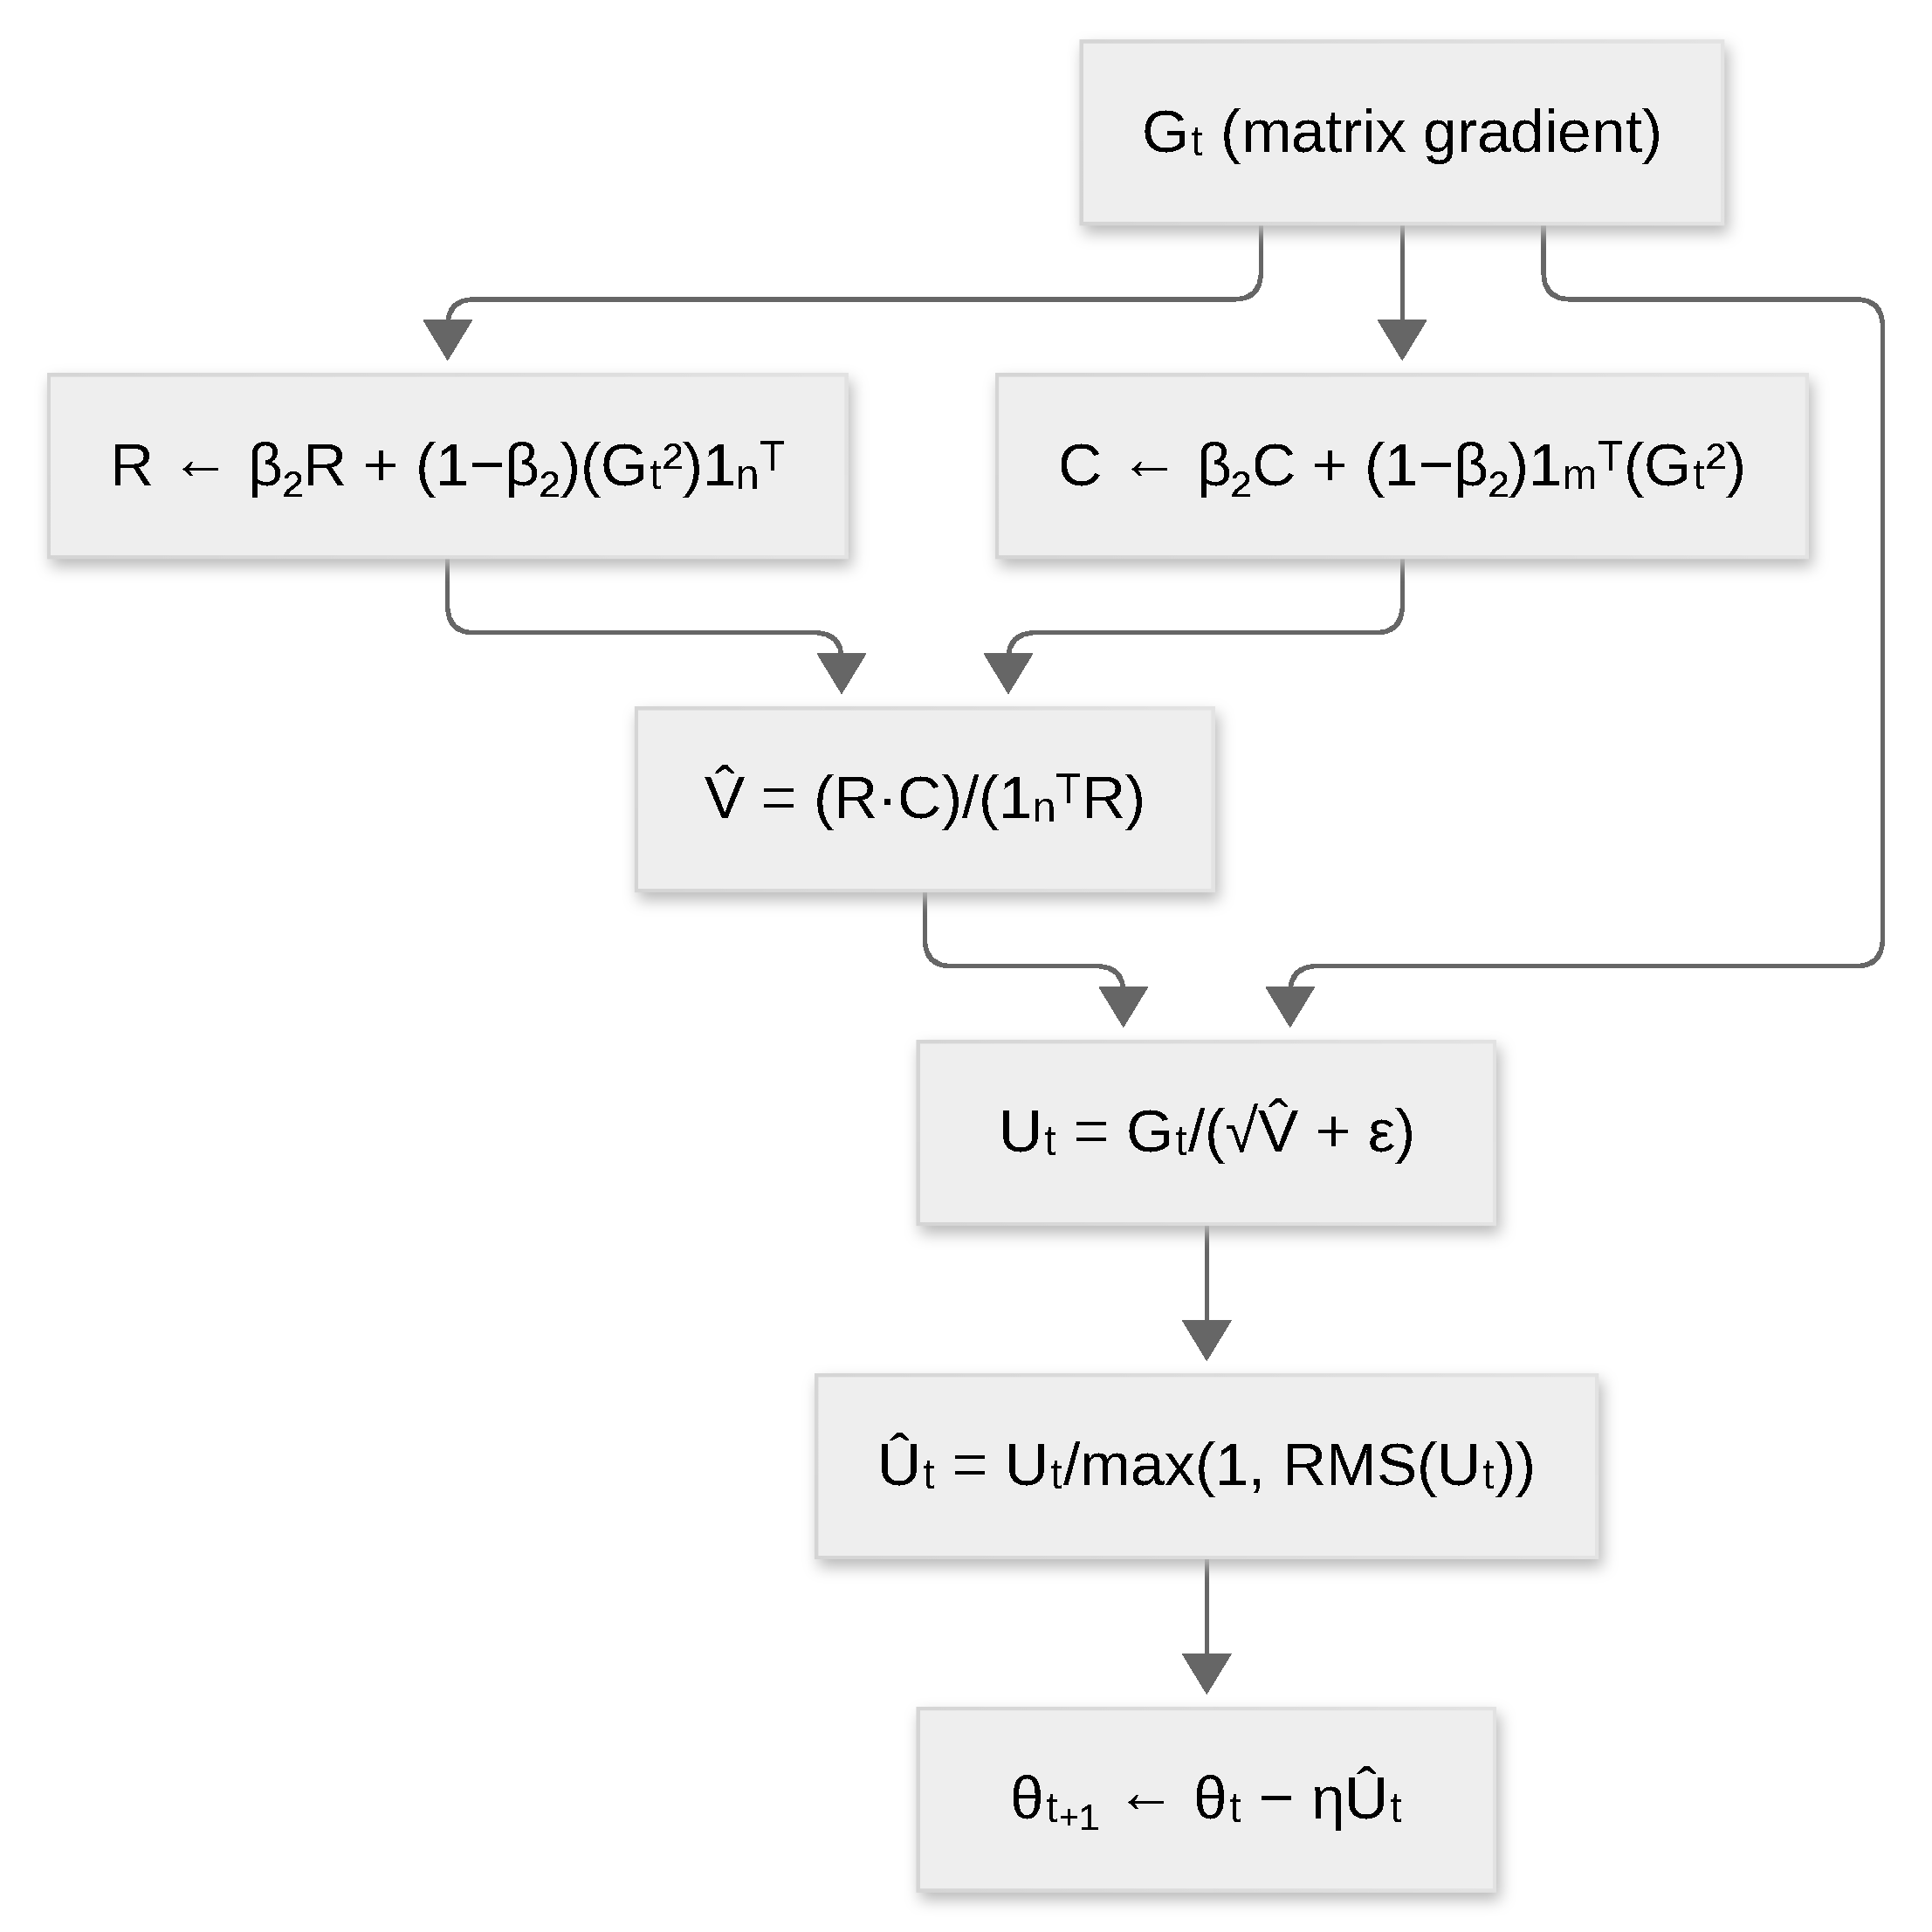
\includegraphics{figures/optimizers/adafactor.pdf}}
\caption{Step flow of Adafactor: factorized row/column second-moment accumulators, outer-product variance reconstruction, and RMS clipping.}
\label{fig:opt-adafactor}
\end{figure}
Adafactor reduces optimizer memory by \textbf{factorizing} second-moment statistics for matrix-shaped parameters, storing only row and column accumulators rather than dense variance states. For a gradient matrix $G_t \in \mathbb{R}^{m \times n}$:
\begin{align}
R_t &= \beta_2 R_{t-1} + (1-\beta_2)(G_t^2) \mathbf{1}_n^T \quad\text{(row variance)} \\
C_t &= \beta_2 C_{t-1} + (1-\beta_2) \mathbf{1}_m^\top (G_t^2) \quad\text{(column variance)} \\
\hat{V}_t &= \frac{R_t C_t}{\mathbf{1}_n^\top R_t} \quad\text{(reconstructed variance via outer product)} \\
U_t &= \frac{G_t}{\sqrt{\hat{V}_t}+\epsilon} \quad\text{(normalized adaptive step)} \\
\hat{U}_t &= \frac{U_t}{\max(1, \text{RMS}(U_t))} \quad\text{(stability clipping)}
\end{align}

\begin{algorithm}[H]
\caption{Adafactor (Factorized Second-Moment Statistics)}
\label{alg:adafactor}
\begin{algorithmic}[1]
\Require Gradient matrix $G_t \in \mathbb{R}^{m \times n}$, learning rate $\eta$, $\beta_2 \approx 0.999$
\Ensure Updated parameters $\theta_T$
\State Initialize: Row accumulators $R \gets \epsilon \mathbf{1}^T_m$, Column $C \gets \epsilon \mathbf{1}_n$
\For{$t = 1, 2, \ldots, T$}
    \State $G_t \gets \nabla f(\theta_t)$ (matrix gradient)
    \State $R \gets \beta_2 R + (1-\beta_2) (G_t^2) \mathbf{1}_n^T$ \Comment{Row inner products}
    \State $C \gets \beta_2 C + (1-\beta_2) \mathbf{1}_m^\top (G_t^2)$ \Comment{Column inner products}
    \State Reconstructed variance: $\hat{V} \gets (R \cdot C) / (\mathbf{1}_n^\top R)$ \Comment{Via outer product}
    \State Normalized adaptive step: $U_t \gets G_t / (\sqrt{\hat{V}} + \epsilon)$
    \State Per-row RMS clipping: $\hat{U}_t \gets U_t / \max(1, \text{RMS}(U_t))$
    \State $\theta_{t+1} \gets \theta_t - \eta \hat{U}_t$
\EndFor
\Return $\theta_T$
\end{algorithmic}
\end{algorithm}

\paragraph{Cons.}
\begin{itemize}[leftmargin=*]
\item Factorized variance is an approximation and can be unstable on some tasks.
\item Reduced optimization expressiveness relative to full Adam.
\end{itemize}

\paragraph{Pros.}
\begin{itemize}[leftmargin=*]
\item Memory drops from $O(n_{\text{params}})$ to $O(\sqrt{n_{\text{params}}})$ for matrix parameters.
\item Most attractive when VRAM is dominated by optimizer state rather than activations.
\end{itemize}

\paragraph{GaLore (Gradient Low-Rank Projection).}
\begin{figure}[H]
\centering
\fitfigure{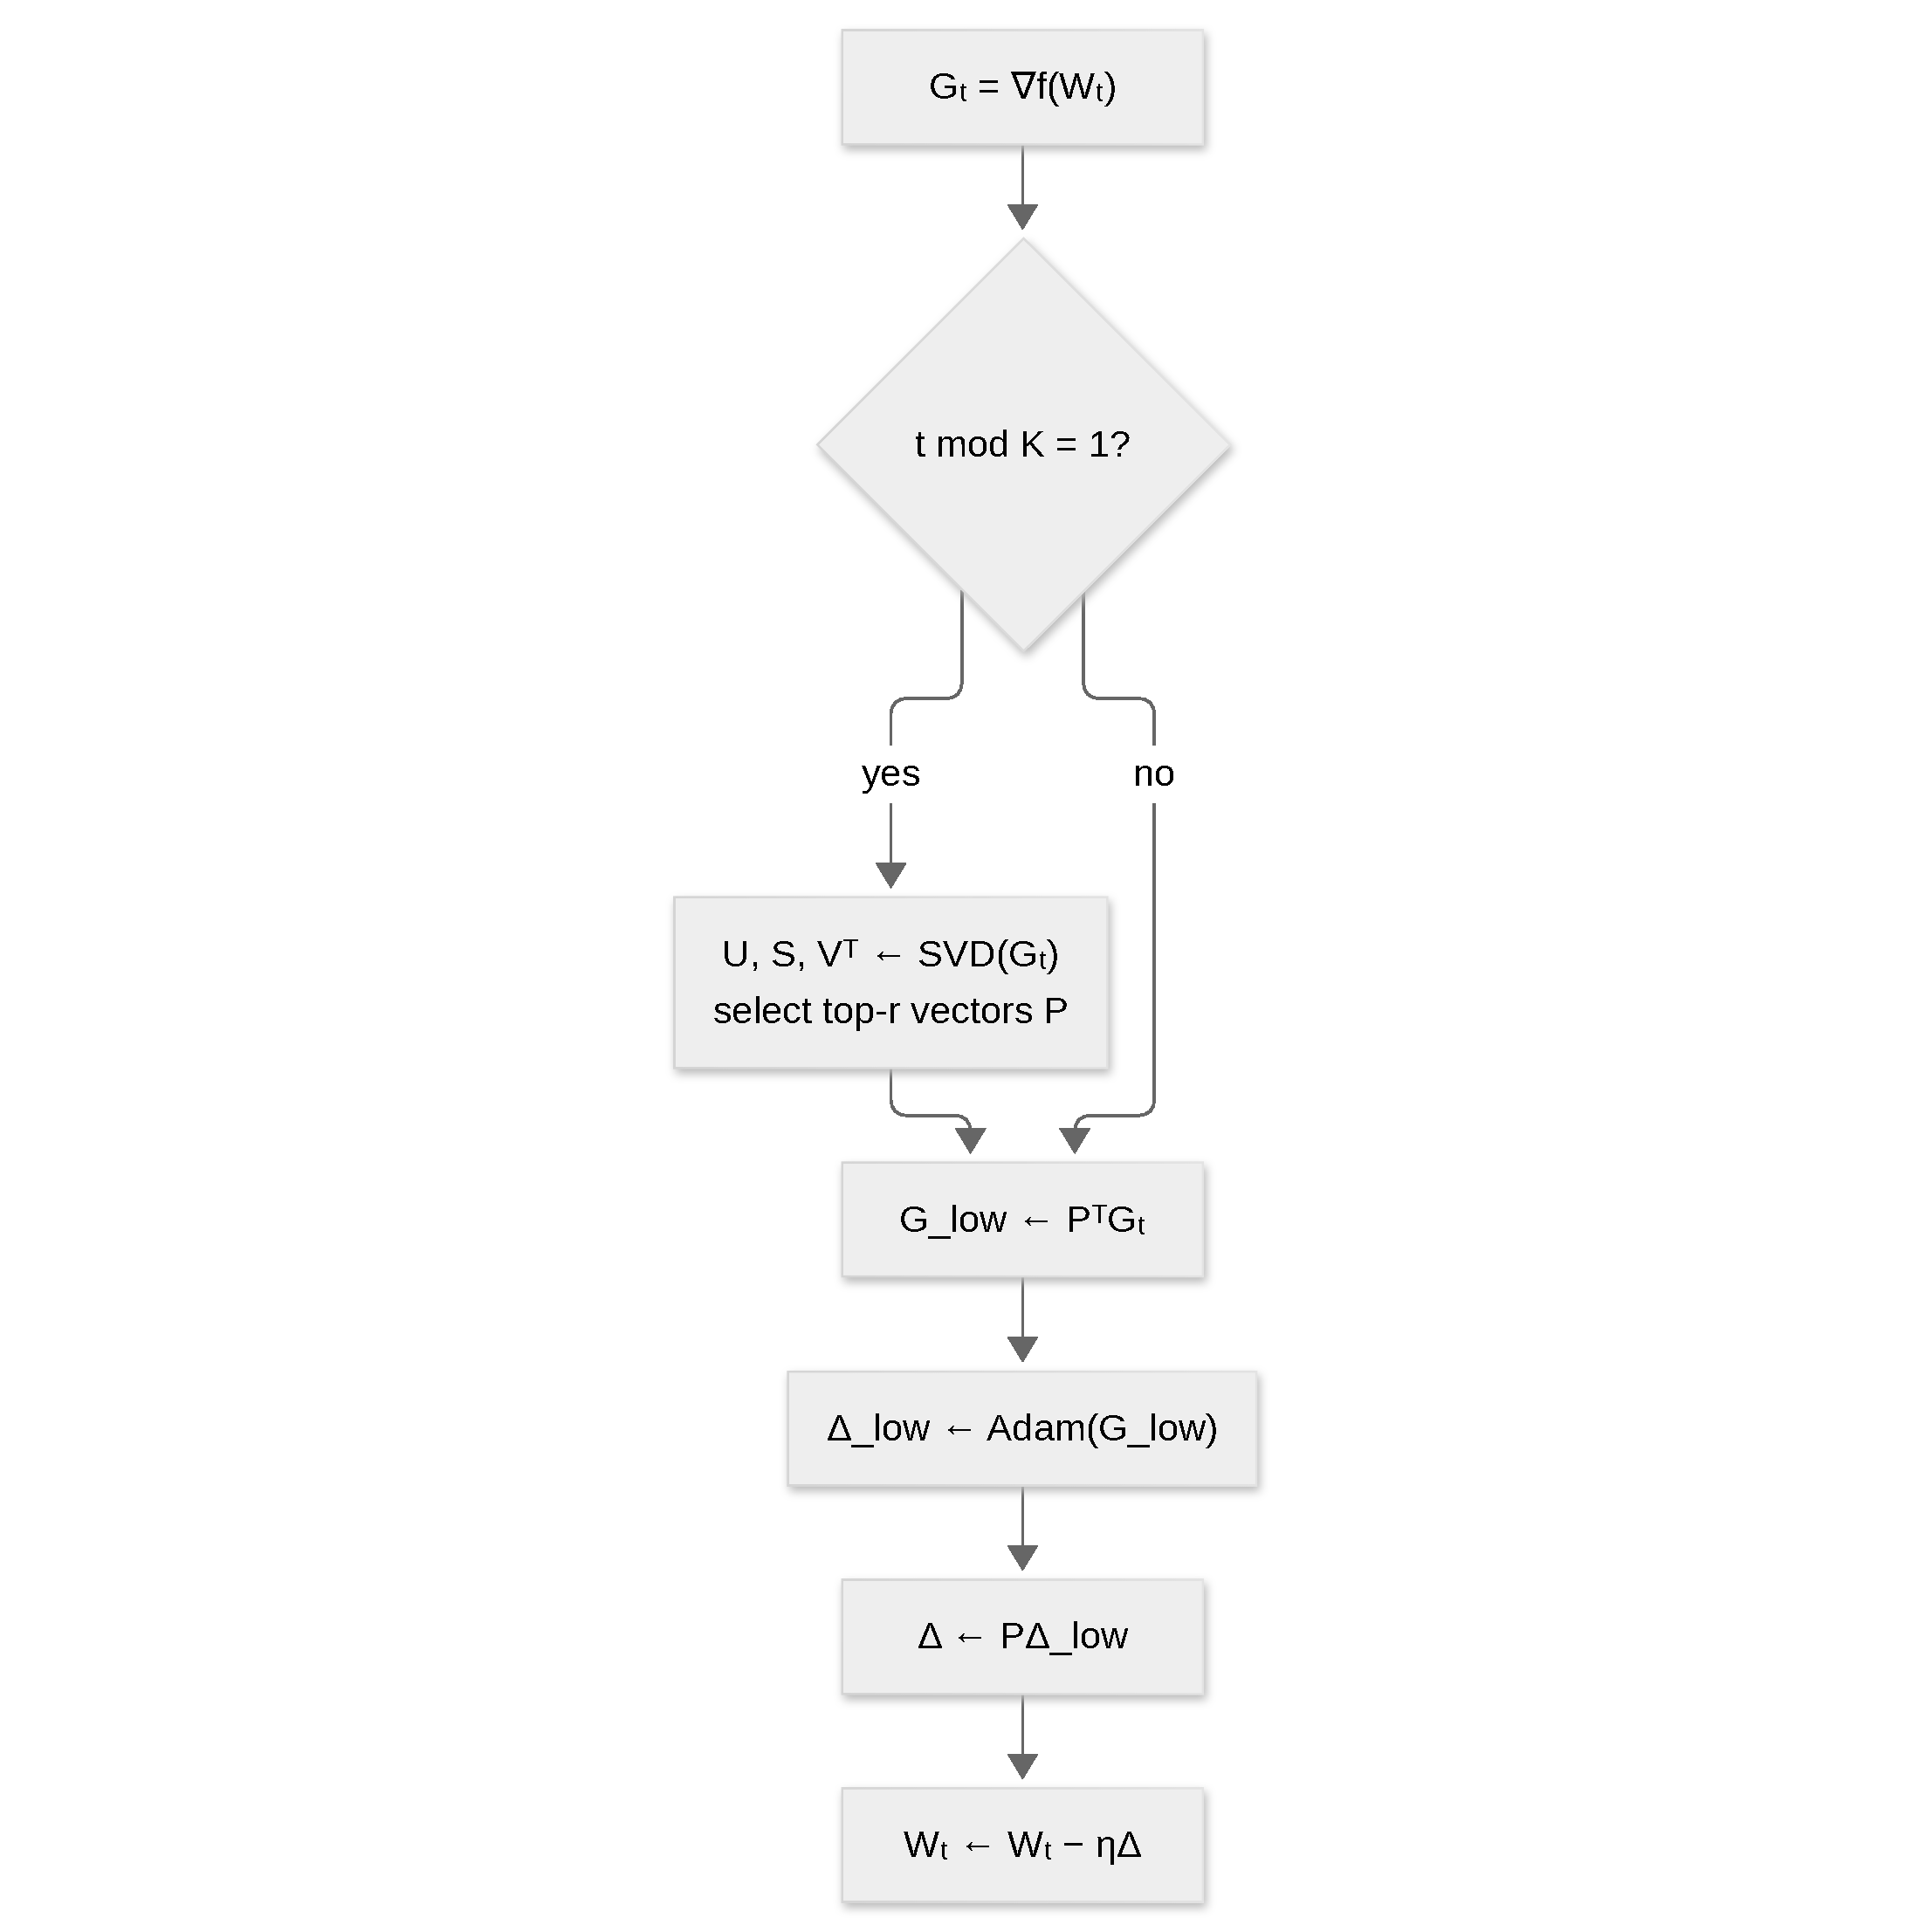
\includegraphics{figures/optimizers/galore.pdf}}
\caption{Step flow of GaLore: periodic SVD projection of the gradient into a low-rank subspace, Adam in that subspace, and reconstruction.}
\label{fig:opt-galore}
\end{figure}
GaLore projects 2D gradients into a low-rank subspace before optimization, reducing optimizer-state memory while maintaining adaptive step scaling. For a 2D parameter matrix $W \in \mathbb{R}^{m \times n}$:
\begin{align}
U, S, V &= \text{SVD}(G_t) \quad\text{(compute singular decomposition)} \\
P &\in \mathbb{R}^{n \times r} \quad\text{or} \quad P^\top \in \mathbb{R}^{r \times m} \quad\text{(select top-$r$ singular vectors)} \\
G_{\text{low}} &= P^\top G_t \quad\text{(project to low-rank space)} \\
\Delta_{\text{low}} &= \text{Adam}(G_{\text{low}}) \quad\text{(optimize in compressed space)} \\
\Delta &= P \Delta_{\text{low}} \quad\text{(reconstruct in original space)}
\end{align}
By projecting into a rank-$r$ subspace (typically $r \ll \min(m,n)$), optimizer state is reduced from $O(mn)$ to $O(r(m+n))$ for 2D parameters. This complementary memory-saving approach is especially relevant when the model is too large for full-rank optimizer state.

\begin{algorithm}[H]
\caption{GaLore (Gradient Low-Rank Projection)}
\label{alg:galore}
\begin{algorithmic}[1]
\Require 2D parameter matrix $W \in \mathbb{R}^{m \times n}$, learning rate $\eta$, rank $r \ll \min(m,n)$
\Ensure Updated parameters $\theta_T$
\State Initialize: Adam state in low-rank space (if rank-2 variant)
\For{$t = 1, 2, \ldots, T$}
    \State $G_t \gets \nabla f(W_t)$
    \If{$t \mod K = 1$}  \Comment{Periodic SVD}
        \State $U_t, S_t, V_t^\top \gets \text{SVD}(G_t)$ (full or thin)
        \State Select projection: $P \gets U_t[:, :r]$ or $P \gets V_t[:, :r]$
    \EndIf
    \State Project gradient: $G_{\text{low}} \gets P^\top G_t$ (or $G_t P^\top$ for right projection)
    \State Run Adam on low-rank: $\Delta_{\text{low}} \gets \text{Adam}(G_{\text{low}})$
    \State Reconstruct in original space: $\Delta \gets P \Delta_{\text{low}}$ (or $\Delta_{\text{low}} P^\top$)
    \State $W_t \gets W_t - \eta \Delta$
\EndFor
\Return $\theta_T$
\end{algorithmic}
\end{algorithm}

\paragraph{Cons.}
\begin{itemize}[leftmargin=*]
\item Periodic SVD adds compute and introduces a projection-refresh interval to tune.
\item Low-rank projection can discard gradient information.
\end{itemize}

\paragraph{Pros.}
\begin{itemize}[leftmargin=*]
\item Optimizer state reduced from $O(mn)$ to $O(r(m+n))$ for 2D parameters.
\item Works synergistically with other techniques and has shown strong results on billion-parameter models.
\end{itemize}

\paragraph{APOLLO, APOLLO-Mini, and Q-APOLLO.}
\begin{figure}[H]
\centering
\fitfigure{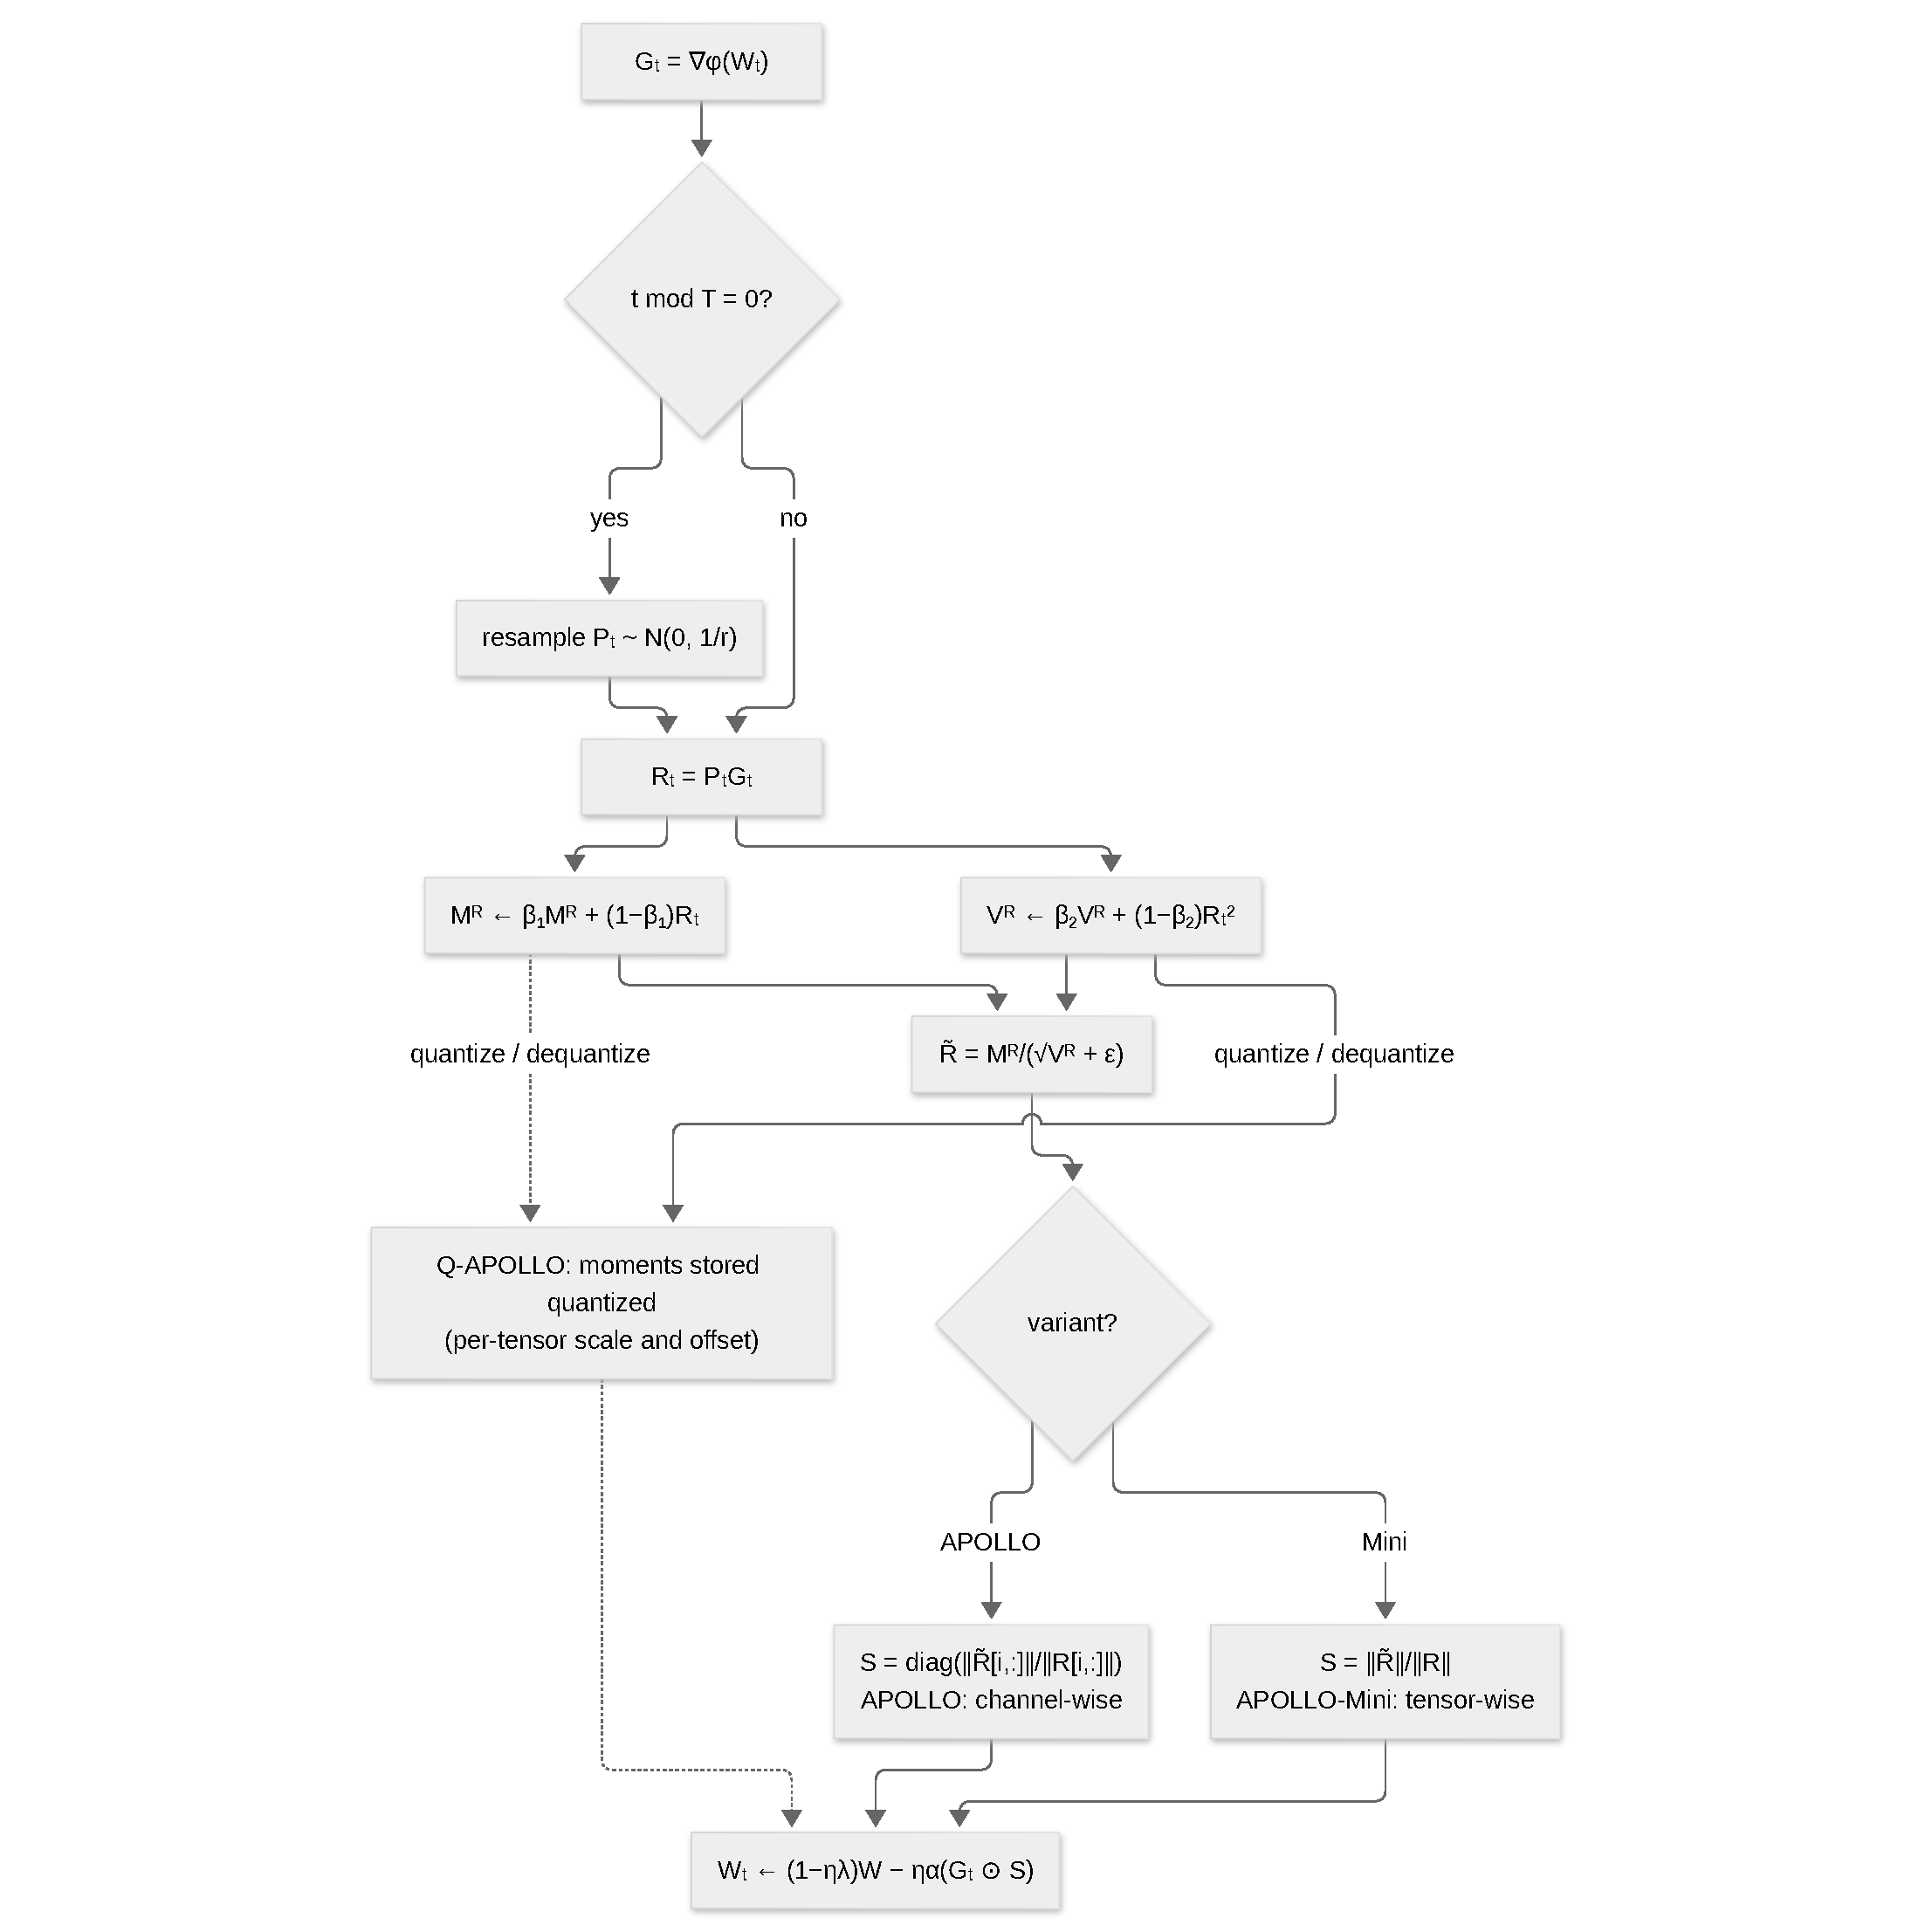
\includegraphics{figures/optimizers/apollo.pdf}}
\caption{Step flow of the APOLLO family: Gaussian-projected moments, structured gradient scaling (channel-wise for APOLLO, scalar for APOLLO-Mini), and quantized state for Q-APOLLO.}
\label{fig:opt-apollo}
\end{figure}
The APOLLO family \citep{zhu2025apollosgdlikememoryadamwlevel} begins from the observation that AdamW's element-wise denominator can be \textbf{coarsened into a structured learning-rate update}. Rather than storing dense moments for every parameter entry, APOLLO projects a matrix gradient $G_t \in \mathbb{R}^{m \times n}$ into a compact random subspace and tracks Adam-style moments there:
\begin{align}
R_t &= P_t G_t \quad\text{or}\quad R_t = G_t P_t^\top \\
M_t^R &= \beta_1 M_{t-1}^R + (1-\beta_1)R_t \\
V_t^R &= \beta_2 V_{t-1}^R + (1-\beta_2)R_t^2 \\
\widetilde{R}_t &= \frac{M_t^R}{\sqrt{V_t^R}+\epsilon}
\end{align}
The projected state is \emph{not} expanded back into a dense low-rank update as in SVD-based methods. Instead, APOLLO estimates a structured scaling tensor $S_t$ in the original space. In the standard APOLLO variant, that scaling is \textbf{channel-wise}: each row or channel receives its own norm ratio. In APOLLO-Mini, the scaling is reduced to a single \textbf{tensor-wise} scalar, corresponding to the rank-1 extreme described in the paper. The resulting parameter update is therefore Adam-like in adaptation but much closer to SGD in state cost:
\[
W_t \gets (1-\eta\lambda)W_{t-1} - \eta\,\alpha\,(G_t \odot S_t)
\]
where $\alpha$ is the extra scale factor used to stabilize highly compressed variants.

\begin{algorithm}[H]
\caption{APOLLO / APOLLO-Mini Structured Gradient Scaling}
\label{alg:apollo-family}
\begin{algorithmic}[1]
\Require Weight matrix $W \in \mathbb{R}^{m \times n}$ with $m \le n$, learning rate $\eta$, scale factor $\alpha$, decay rates $(\beta_1, \beta_2)$, weight decay $\lambda$, rank $r$, projection refresh interval $T$
\Ensure Updated parameters $W_T$
\State Initialize projected moments: $M^R \gets 0$, $V^R \gets 0$, step $t \gets 0$
\Repeat
    \State Compute gradient: $G_t \gets \nabla_W \phi(W_t)$
    \If{$t \bmod T = 0$}
        \State Sample Gaussian projector $P_t \sim \mathcal{N}(0, 1/r)$ with a fresh seed
    \EndIf
    \State Project gradient: $R_t \gets P_t G_t$ \Comment{or $G_t P_t^\top$ depending on layout}
    \State Update projected AdamW moments: $M_t^R, V_t^R \gets \text{AdamWState}(R_t; \beta_1, \beta_2)$
    \State Normalize projected state: $\widetilde{R}_t \gets M_t^R / (\sqrt{V_t^R}+\epsilon)$
    \If{APOLLO}
        \State $S_t \gets \operatorname{diag}(s_1^R, \ldots, s_m^R)$, where $s_i^R = \|\widetilde{R}_t[i,:]\|_2 / \|R_t[i,:]\|_2$
    \Else
        \State $S_t \gets s_t^R$, where $s_t^R = \|\widetilde{R}_t\|_2 / \|R_t\|_2$
    \EndIf
    \State Update weights: $W_t \gets (1-\eta\lambda)W_{t-1} - \eta\,\alpha\,(G_t \odot S_t)$
    \State $t \gets t+1$
\Until{convergence}
\end{algorithmic}
\end{algorithm}

\paragraph{Cons.}
\begin{itemize}[leftmargin=*]
\item Structured scaling is a coarser approximation of AdamW's element-wise denominator.
\item Projectors must be refreshed periodically, and very small ranks make the scaling noisy.
\end{itemize}

\paragraph{Pros.}
\begin{itemize}[leftmargin=*]
\item Replaces repeated SVD with periodically refreshed Gaussian random projection, so the systems cost is ordinary matrix multiplication rather than spectral decomposition.
\item Unusually tolerant to extreme compression: even APOLLO-Mini, which keeps only rank-1 auxiliary state, remains competitive with or better than AdamW while approaching SGD-level memory.
\end{itemize}

\paragraph{APOLLO-Mini.}
APOLLO-Mini is the family member optimized for \textbf{extreme memory efficiency}. The paper motivates it by arguing that, in a rank-1 compact space, channel-wise scaling becomes too noisy, so the update is coarsened further to a single tensor-wise scale. The loss of granularity is partially offset by the explicit scaling factor $\alpha$ (the paper discusses values such as $128$ in this regime), giving a useful point on the optimization Pareto frontier: very small state, no SVD overhead, and still strong pre-training behavior.

\paragraph{Cons.}
\begin{itemize}[leftmargin=*]
\item A single tensor-wise scale loses channel granularity, and rank-1 state can be noisy.
\item Depends on the extra scale factor $\alpha$ (e.g., $128$) to remain stable.
\end{itemize}

\paragraph{Pros.}
\begin{itemize}[leftmargin=*]
\item Smallest state in the APOLLO family, with no SVD overhead.
\item Strong pre-training behavior at near-SGD memory cost.
\end{itemize}

\paragraph{Q-APOLLO.}
The APOLLO paper also stresses that the family combines naturally with \textbf{quantization} for ultra-low-memory training. This repository turns that systems observation into a concrete optimizer variant, \texttt{q\_apollo}. In the implementation, APOLLO's low-rank first and second moments are stored in quantized form together with per-tensor scales and offsets, and are dequantized only when needed for the next step. Q-APOLLO therefore preserves APOLLO's projected-gradient logic while reducing the precision of the remaining optimizer state.

\paragraph{Cons.}
\begin{itemize}[leftmargin=*]
\item Quantized moments introduce approximation error and dequantization overhead.
\item Requires managing per-tensor scales and offsets.
\end{itemize}

\paragraph{Pros.}
\begin{itemize}[leftmargin=*]
\item Reduces the remaining optimizer state to ultra-low precision.
\item Most aggressive memory-saving member of the local optimizer stack while preserving APOLLO's projected-gradient logic.
\end{itemize}

\paragraph{Anon (Adaptivity Non-restricted Optimizer with Novel convergence technique).}
\begin{figure}[H]
\centering
\fitfigure{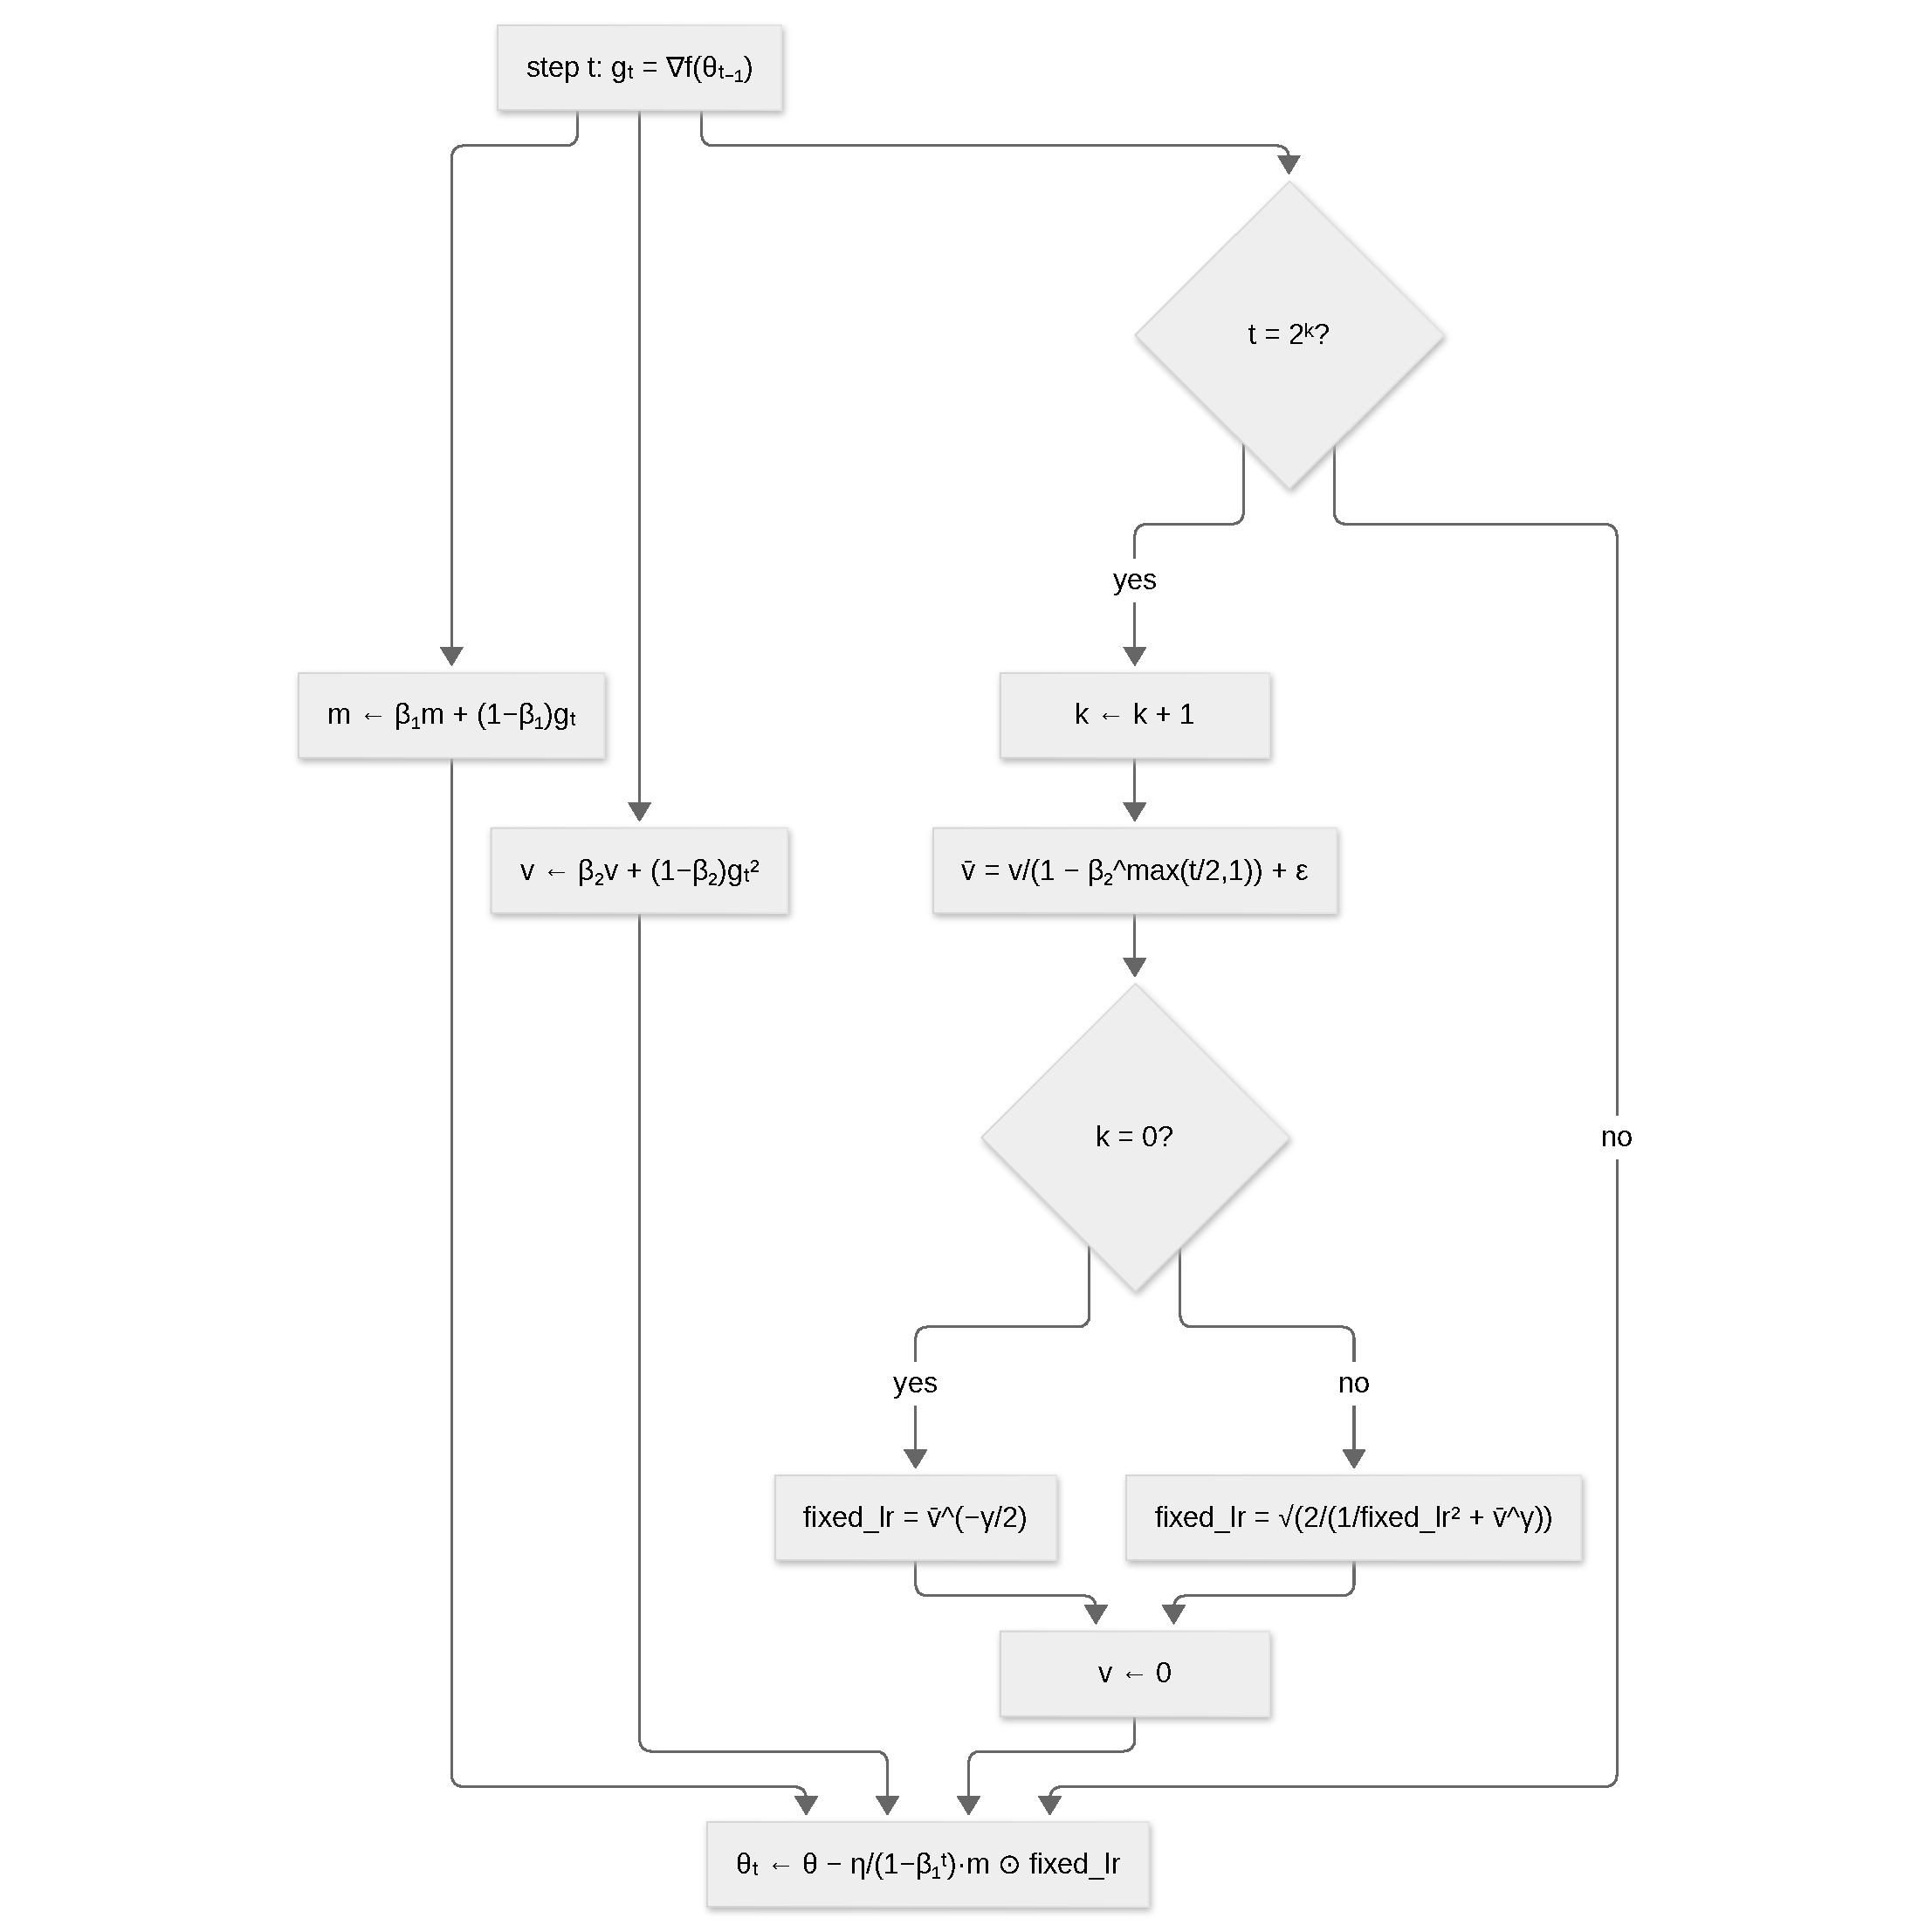
\includegraphics{figures/optimizers/anon.pdf}}
\caption{Step flow of Anon: the IDU preconditioner refreshed at powers of two, with tunable adaptivity $\gamma$ and a bias-corrected momentum update.}
\label{fig:opt-anon}
\end{figure}
Anon \citep{anon2026anon} introduces continuously tunable adaptivity via a single parameter $\gamma \in \mathbb{R}$, bridging the gap between SGD-like ($\gamma=0$) and Adam-like ($\gamma=1$) behaviors, and extrapolating beyond both. The core innovation is the Incremental Delay Update (IDU) mechanism, which enables stable convergence across the entire real-valued adaptivity spectrum:

\begin{align}
m_t &= \beta_1 m_{t-1} + (1-\beta_1) g_t \quad\text{(first moment)}\\
v_t &= \beta_2 v_{t-1} + (1-\beta_2) g_t^2 \quad\text{(second moment)}\\
\bar{v}_t &= \frac{v_t}{1-\beta_2^{\max(t,1)}} + \epsilon \quad\text{(bias-corrected second moment)}\\
\text{fixed\_lr}_k &= \begin{cases}
\bar{v}_k^{-\gamma/2} & \text{if } k = 0 \\
\sqrt{2 / \left(\frac{1}{\text{fixed\_lr}_{k-1}^2} + \bar{v}_k^\gamma\right)} & \text{if } k > 0
\end{cases}\\
\theta_{t+1} &= \theta_t - \frac{\eta}{1-\beta_1^t} \cdot m_t \odot \text{fixed\_lr}_{\lfloor\log_2 t\rfloor}
\end{align}

Unlike standard adaptive optimizers, IDU updates the preconditioner only at powers of two ($t = 2^k$), accumulating gradient statistics between updates and aggregating them recursively. This soft, multi-scale accumulator avoids the hard max-tracking of AMSGrad while provably stabilizing convergence for any $\gamma \in \mathbb{R}$. The parameter $\gamma$ directly controls adaptivity: $\gamma > 1$ accelerates escape from saddle points (favorable for complex architectures), $\gamma = 1$ recovers Adam-like behavior, $\gamma = 0$ yields SGD-like scaling, and $\gamma < 0$ biases toward flatter minima (beneficial for classical architectures like CNNs).

\begin{algorithm}[H]
\caption{Anon (Adaptivity Non-restricted Optimizer with IDU)}
\label{alg:anon}
\begin{algorithmic}[1]
\Require Initial parameters $\theta_0$, learning rate $\eta$, $\beta_1, \beta_2$, tolerance $\epsilon$, adaptivity $\gamma \in \mathbb{R}$
\Ensure Updated parameters $\theta_T$
\State Initialize: $m \gets 0$, $v \gets 0$, fixed\_lr $\gets 0$, step $t \gets 0$, IDU counter $k \gets -1$
\For{$t = 1, 2, \ldots, T$}
    \State $g_t \gets \nabla f(\theta_{t-1})$
    \State $m \gets \beta_1 m + (1-\beta_1) g_t$
    \State $v \gets \beta_2 v + (1-\beta_2) g_t^2$
    \If{$t = 2^k$}
        \State $k \gets k+1$
        \State $\bar{v} \gets v/(1 - \beta_2^{\max(t/2,1)}) + \epsilon$
        \If{$k = 0$}
            \State fixed\_lr $\gets \bar{v}^{-\gamma/2}$
        \Else
            \State fixed\_lr $\gets \sqrt{2 / (1/\text{fixed\_lr}^2 + \bar{v}^\gamma)}$
        \EndIf
        \State $v \gets 0$
    \EndIf
    \State $\theta_t \gets \theta_{t-1} - \frac{\eta}{1-\beta_1^t} \cdot m \odot \text{fixed\_lr}$
\EndFor
\Return $\theta_T$
\end{algorithmic}
\end{algorithm}

\paragraph{Cons.}
\begin{itemize}[leftmargin=*]
\item Maintains three state buffers ($m$, $v$, fixed\_lr) and refreshes the preconditioner on a logarithmic schedule.
\item The adaptivity parameter $\gamma$ must be selected per architecture.
\end{itemize}

\paragraph{Pros.}
\begin{itemize}[leftmargin=*]
\item Same $\mathcal{O}(n)$ per-step complexity class as AdamW, with continuously tunable adaptivity.
\item IDU provably attains $\mathcal{O}(\sqrt{T})$ regret for convex problems and $\mathcal{O}(\ln T / \sqrt{T})$ for non-convex settings.
\end{itemize}

\paragraph{Prodigy (Approximating the Distance Estimate).}
\begin{figure}[H]
\centering
\fitfigure{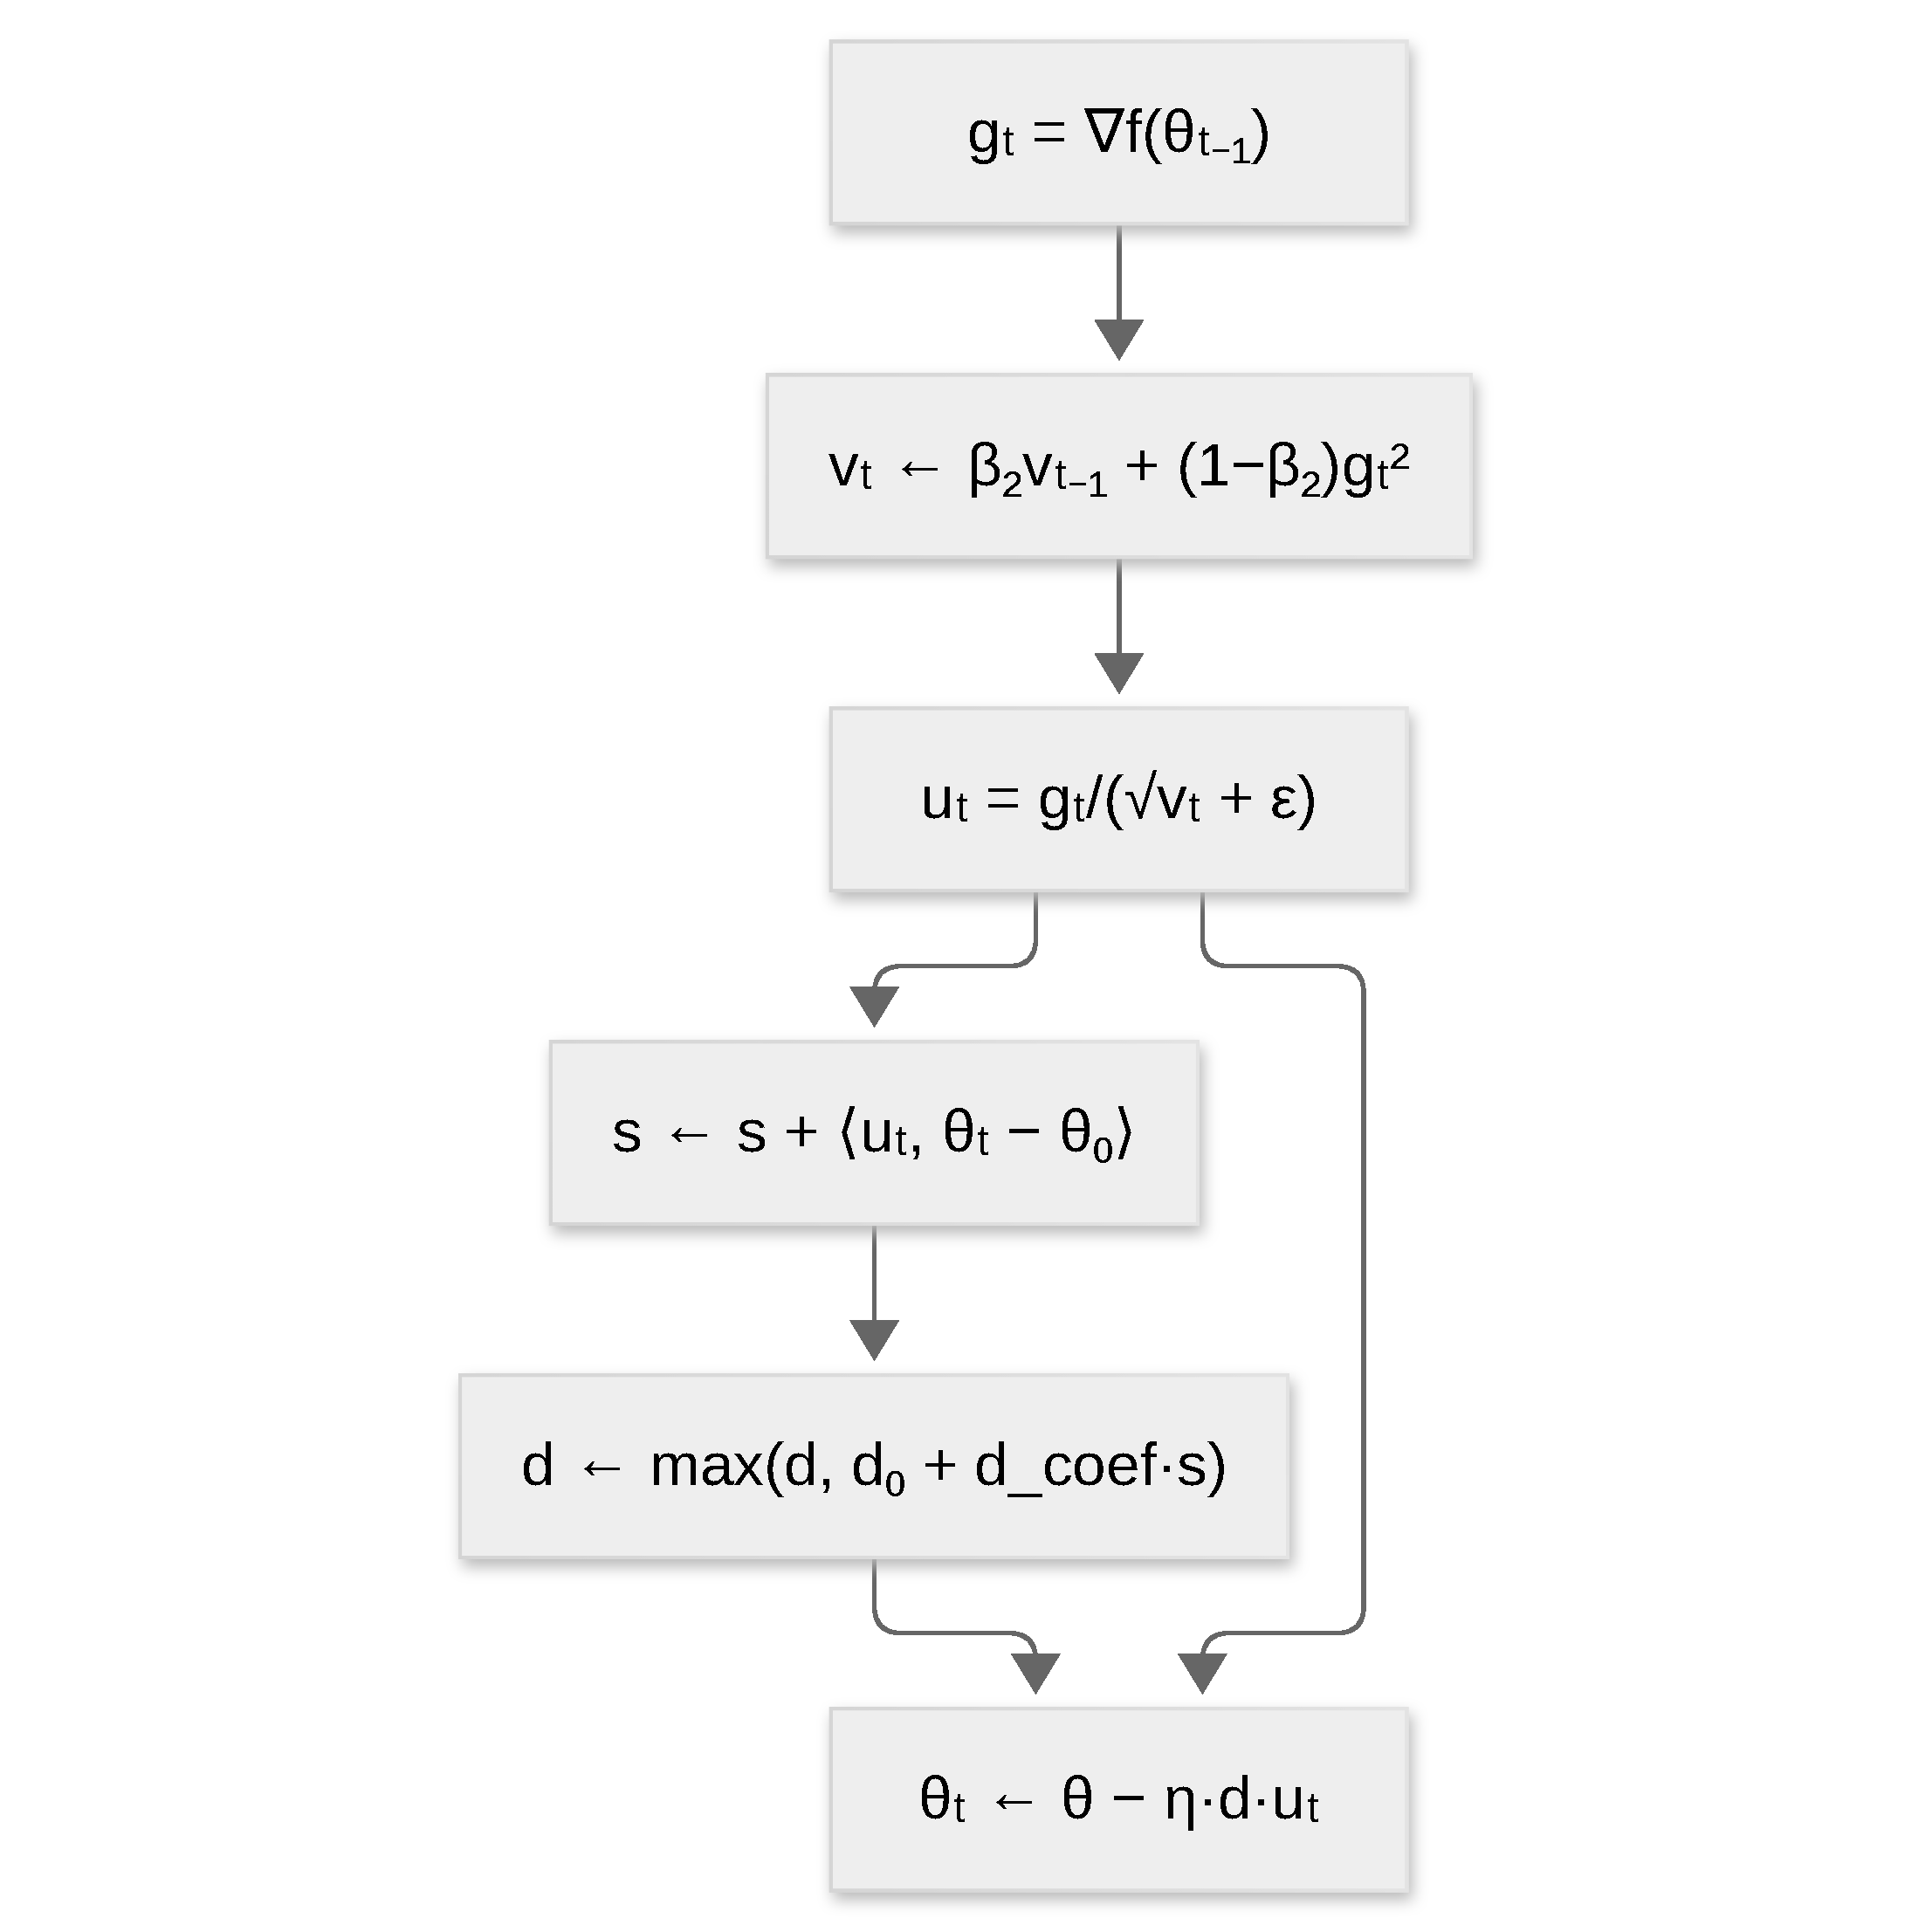
\includegraphics{figures/optimizers/prodigy.pdf}}
\caption{Step flow of Prodigy: a cumulative signed-distance estimate that scales the adaptive step without a learning-rate schedule.}
\label{fig:opt-prodigy}
\end{figure}
Prodigy adapts the effective step scale through a running distance-like statistic, eliminating the need for explicit learning-rate tuning. The algorithm maintains a cumulative distance estimate:
\begin{align}
u_t &= \frac{g_t}{\sqrt{v_t}+\epsilon} \quad\text{(unnormalized adaptive step)} \\
s_t &= s_{t-1} + \langle u_t, \theta_t - \theta_0 \rangle \quad\text{(cumulative signed distance)} \\
d_t &= \max(d_{t-1}, d_0 + d_{\text{coef}} \cdot s_t) \quad\text{(distance estimate with lower bound)} \\
\theta_{t+1} &= \theta_t - \eta \cdot d_t \cdot u_t
\end{align}
where $d_0$ is an initial bound and $d_{\text{coef}}$ controls how aggressively the estimate adapts. The distance estimate $d_t$ captures the combined magnitude of past gradients weighted by actual parameter displacement, implementing an implicit effective learning rate.

\begin{algorithm}[H]
\caption{Prodigy (Approximating the Distance Estimate)}
\label{alg:prodigy}
\begin{algorithmic}[1]
\Require Initial parameters $\theta_0$, learning rate $\eta$, coeff $d_{\text{coef}}$, initial dist $d_0 > 0$
\Ensure Updated parameters $\theta_T$
\State Initialize: $s \gets 0$ (cumulative signed distance), $d \gets d_0$
\For{$t = 1, 2, \ldots, T$}
    \State $g_t \gets \nabla f(\theta_{t-1})$
    \State $v_t \gets \beta_2 v_{t-1} + (1-\beta_2) g_t^2$ \Comment{Second moment}
    \State $u_t \gets g_t / (\sqrt{v_t} + \epsilon)$ \Comment{Unnormalized adaptive}
    \State Update distance: $s \gets s + \langle u_t, \theta_t - \theta_0 \rangle$ \Comment{Signed distance}
    \State $d \gets \max(d, d_0 + d_{\text{coef}} \cdot s)$ \Comment{Lower-bounded distance}
    \State $\theta_t \gets \theta_{t-1} - \eta \cdot d \cdot u_t$ \Comment{Distance-scaled update}
\EndFor
\Return $\theta_T$
\end{algorithmic}
\end{algorithm}

\paragraph{Cons.}
\begin{itemize}[leftmargin=*]
\item Introduces $d_0$ and $d_{\text{coef}}$ hyperparameters for the distance estimate.
\item Adds an inner-product bookkeeping step per iteration.
\end{itemize}

\paragraph{Pros.}
\begin{itemize}[leftmargin=*]
\item Removes explicit learning-rate tuning and scheduling.
\item Robust convergence across problem scales and batch sizes.
\end{itemize}

\subsection{Second-Order, Geometric, and Orthogonality Optimizers}
\paragraph{Shampoo (Matrix Preconditioning via Kronecker Products).}
\begin{figure}[H]
\centering
\fitfigure{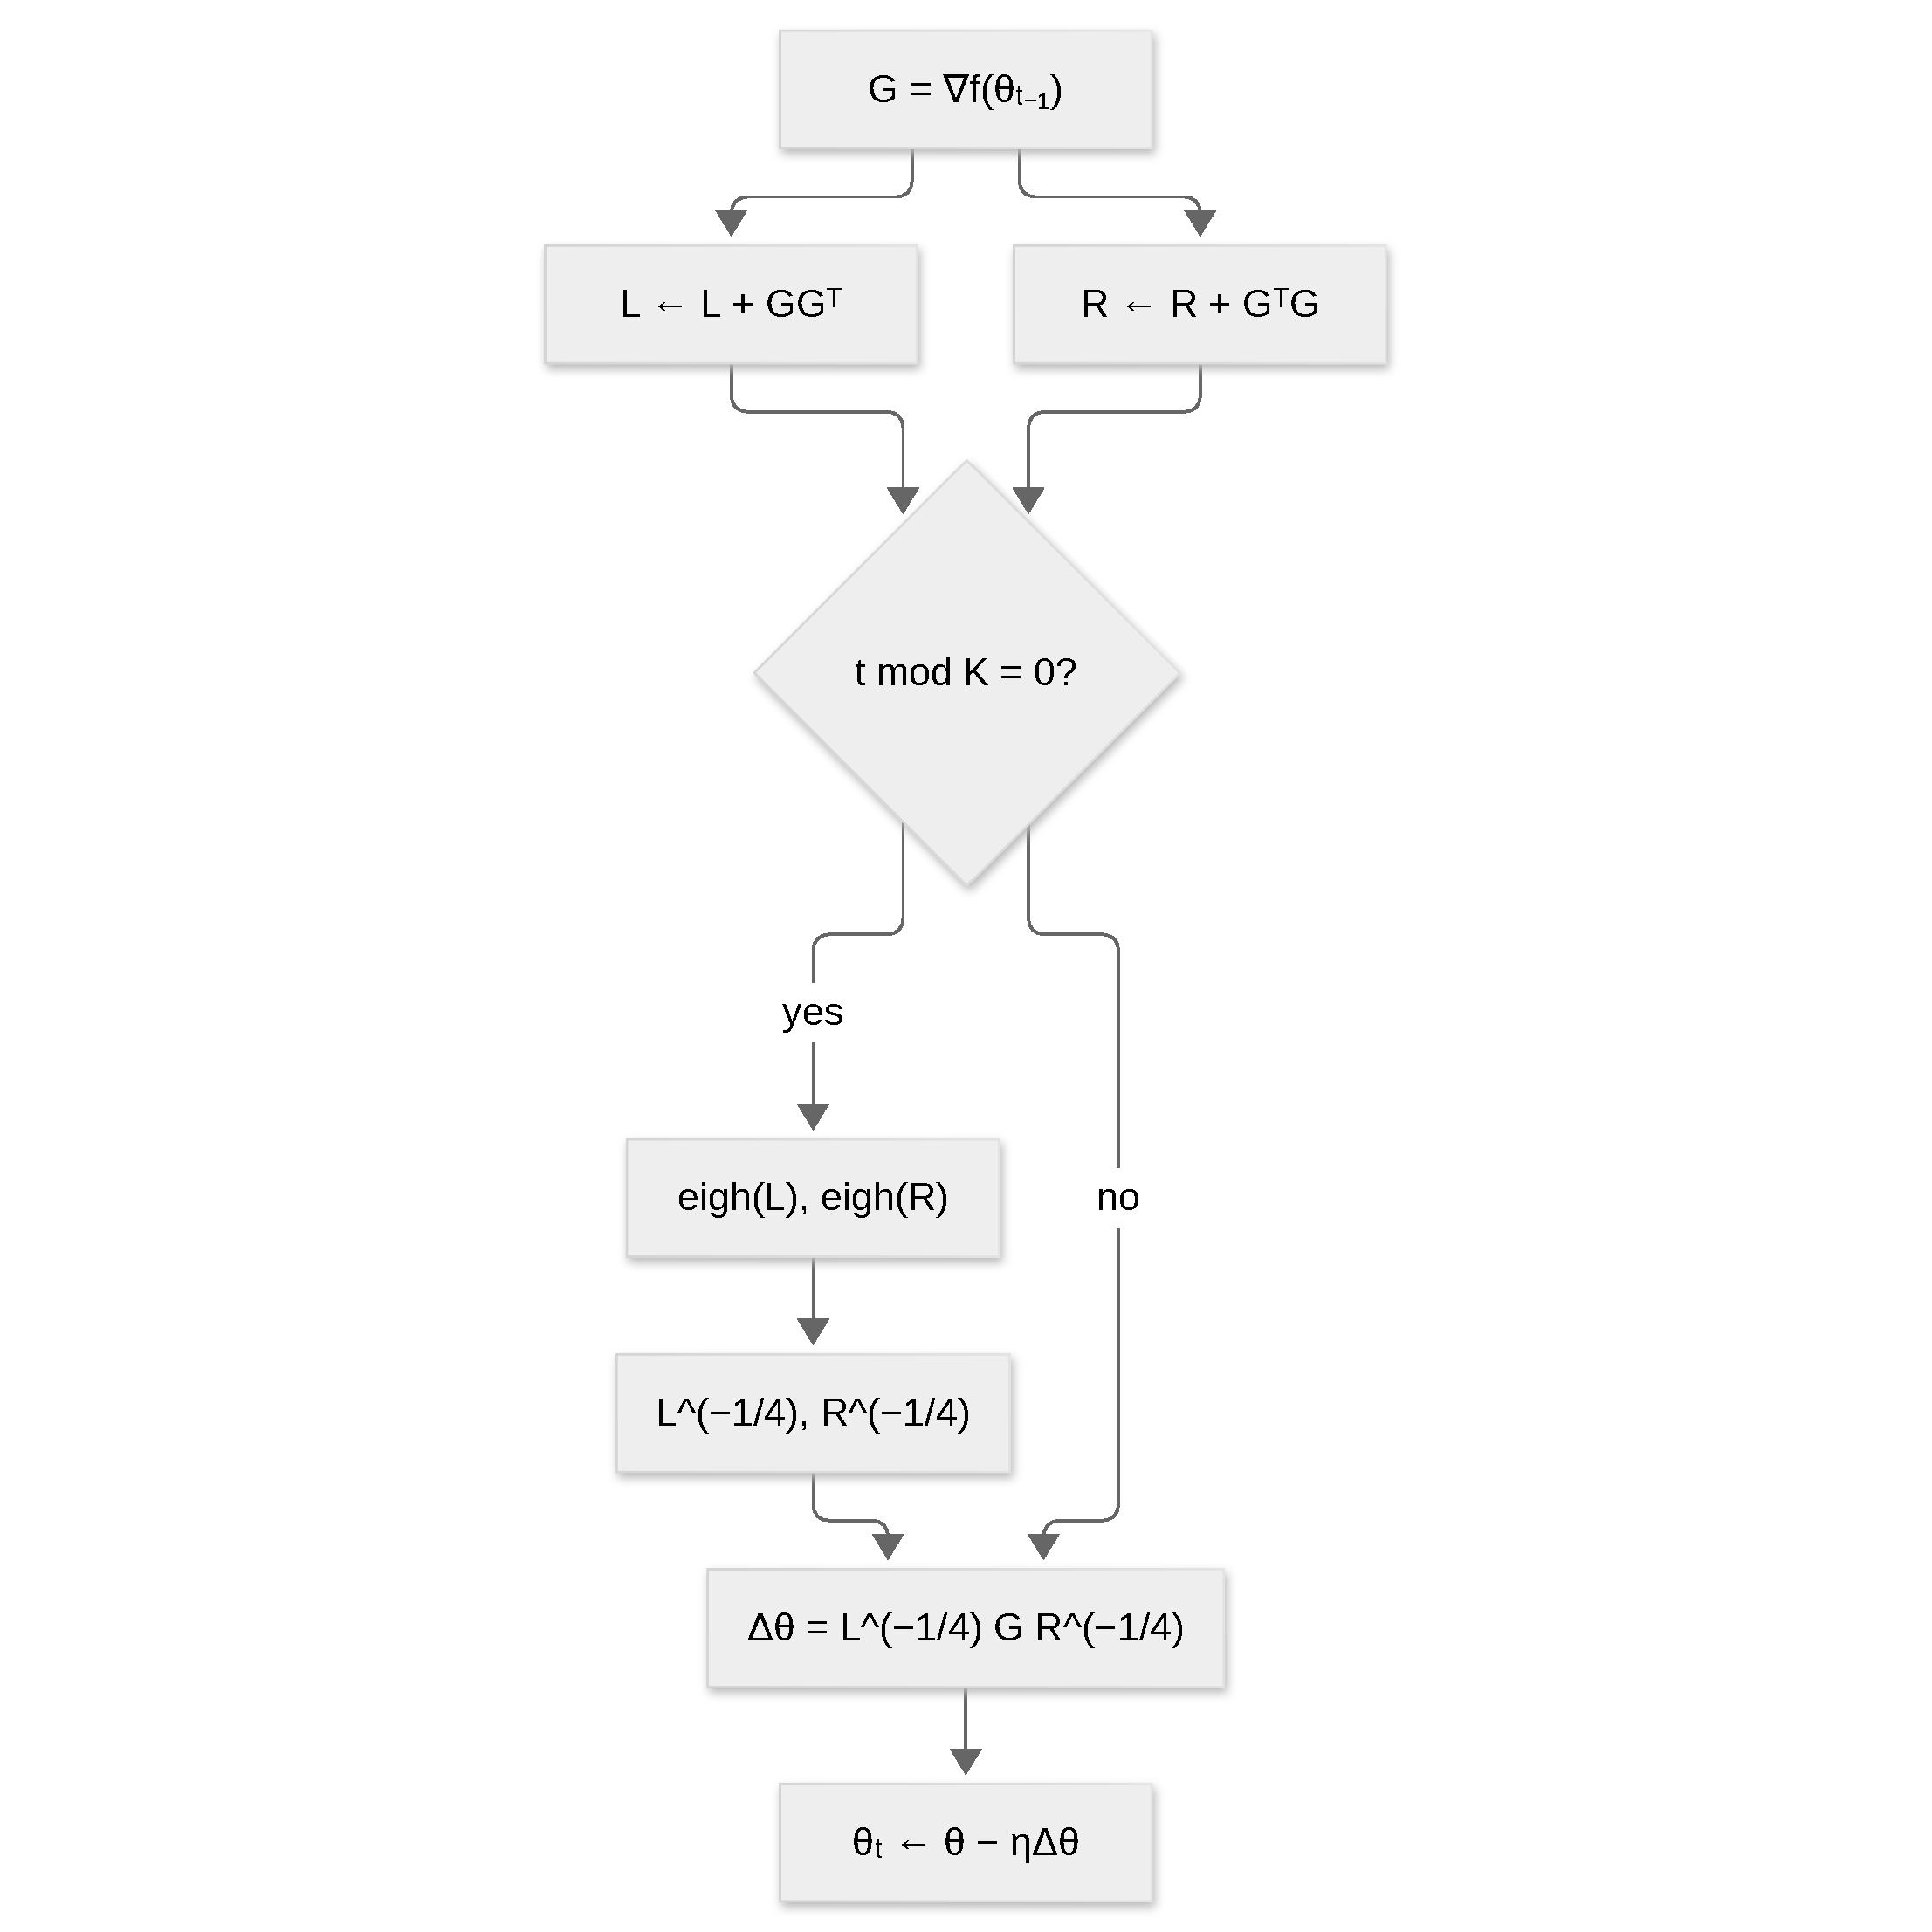
\includegraphics{figures/optimizers/shampoo.pdf}}
\caption{Step flow of Shampoo: Kronecker-factored Gram matrices, periodic eigendecomposition, and fourth-root preconditioning of the gradient.}
\label{fig:opt-shampoo}
\end{figure}
Shampoo is a \textbf{structured second-order method} that computes matrix preconditioners from Kronecker-structured outer-product statistics. For a 2D parameter matrix $W \in \mathbb{R}^{m \times n}$:
\begin{align}
L_t &= L_{t-1} + G_t G_t^\top \quad\text{(left/row Gram matrix, $m \times m$)} \\
R_t &= R_{t-1} + G_t^\top G_t \quad\text{(right/column Gram matrix, $n \times n$)} \\
L_t^{-1/4} &= Q_L (\Lambda_L)^{-1/4} Q_L^\top \quad\text{(via eigendecomposition)} \\
R_t^{-1/4} &= Q_R (\Lambda_R)^{-1/4} Q_R^\top \\
\Delta W_t &= L_t^{-1/4} G_t R_t^{-1/4} \quad\text{(preconditioned gradient)}
\end{align}
Shampoo approximates the full-matrix Adagrad preconditioner $H^{-1/2}$ (where $H$ is the Hessian) using Kronecker-factored structure. Instead of storing a $(mn) \times (mn)$ preconditioner, Shampoo maintains two smaller matrices ($m \times m$ and $n \times n$), capturing cross-parameter correlations within and across groups. Eigendecompositions are performed periodically (e.g., every $K=10$ steps) to amortize cost.

\begin{algorithm}[H]
\caption{Shampoo (Matrix Preconditioning via Kronecker Products)}
\label{alg:shampoo}
\begin{algorithmic}[1]
\Require Initial parameters $\theta_0$, learning rate $\eta$, eigendecomposition interval $K$
\Ensure Updated parameters $\theta_T$
\State Initialize: $L \gets \epsilon I_m$, $R \gets \epsilon I_n$ (left and right Gram matrices)
\For{$t = 1, 2, \ldots, T$}
    \State $G \gets \nabla f(\theta_{t-1})$ \Comment{Gradient}
    \State Update Gram matrices: $L \gets L + G G^\top$, $R \gets R + G^\top G$
    \If{$t \mod K == 0$}
        \State $Q_L, \Lambda_L \gets \text{eigh}(L)$ \Comment{Eigendecomposition of $L$}
        \State $Q_R, \Lambda_R \gets \text{eigh}(R)$ \Comment{Eigendecomposition of $R$}
        \State $L^{-1/4} \gets Q_L (\Lambda_L + \epsilon)^{-1/4} Q_L^\top$
        \State $R^{-1/4} \gets Q_R (\Lambda_R + \epsilon)^{-1/4} Q_R^\top$
    \EndIf
    \State $\Delta \theta \gets L^{-1/4} G R^{-1/4}$ \Comment{Preconditioned gradient}
    \State $\theta_t \gets \theta_{t-1} - \eta \cdot \Delta \theta$
\EndFor
\Return $\theta_T$
\end{algorithmic}
\end{algorithm}

\paragraph{Cons.}
\begin{itemize}[leftmargin=*]
\item Periodic $O(m^3 + n^3)$ eigendecompositions and higher per-step compute.
\item Assumes 2D parameter structure; embeddings and biases need separate handling.
\end{itemize}

\paragraph{Pros.}
\begin{itemize}[leftmargin=*]
\item Kronecker-factored second-order preconditioning without a dense $(mn) \times (mn)$ matrix.
\item Proven effective at production scale and well suited to high-rank transformer matrices, with improved conditioning and accelerated convergence.
\end{itemize}

\paragraph{SOAP (Shampoo with Adam in eigenbasis).}
\begin{figure}[H]
\centering
\fitfigure{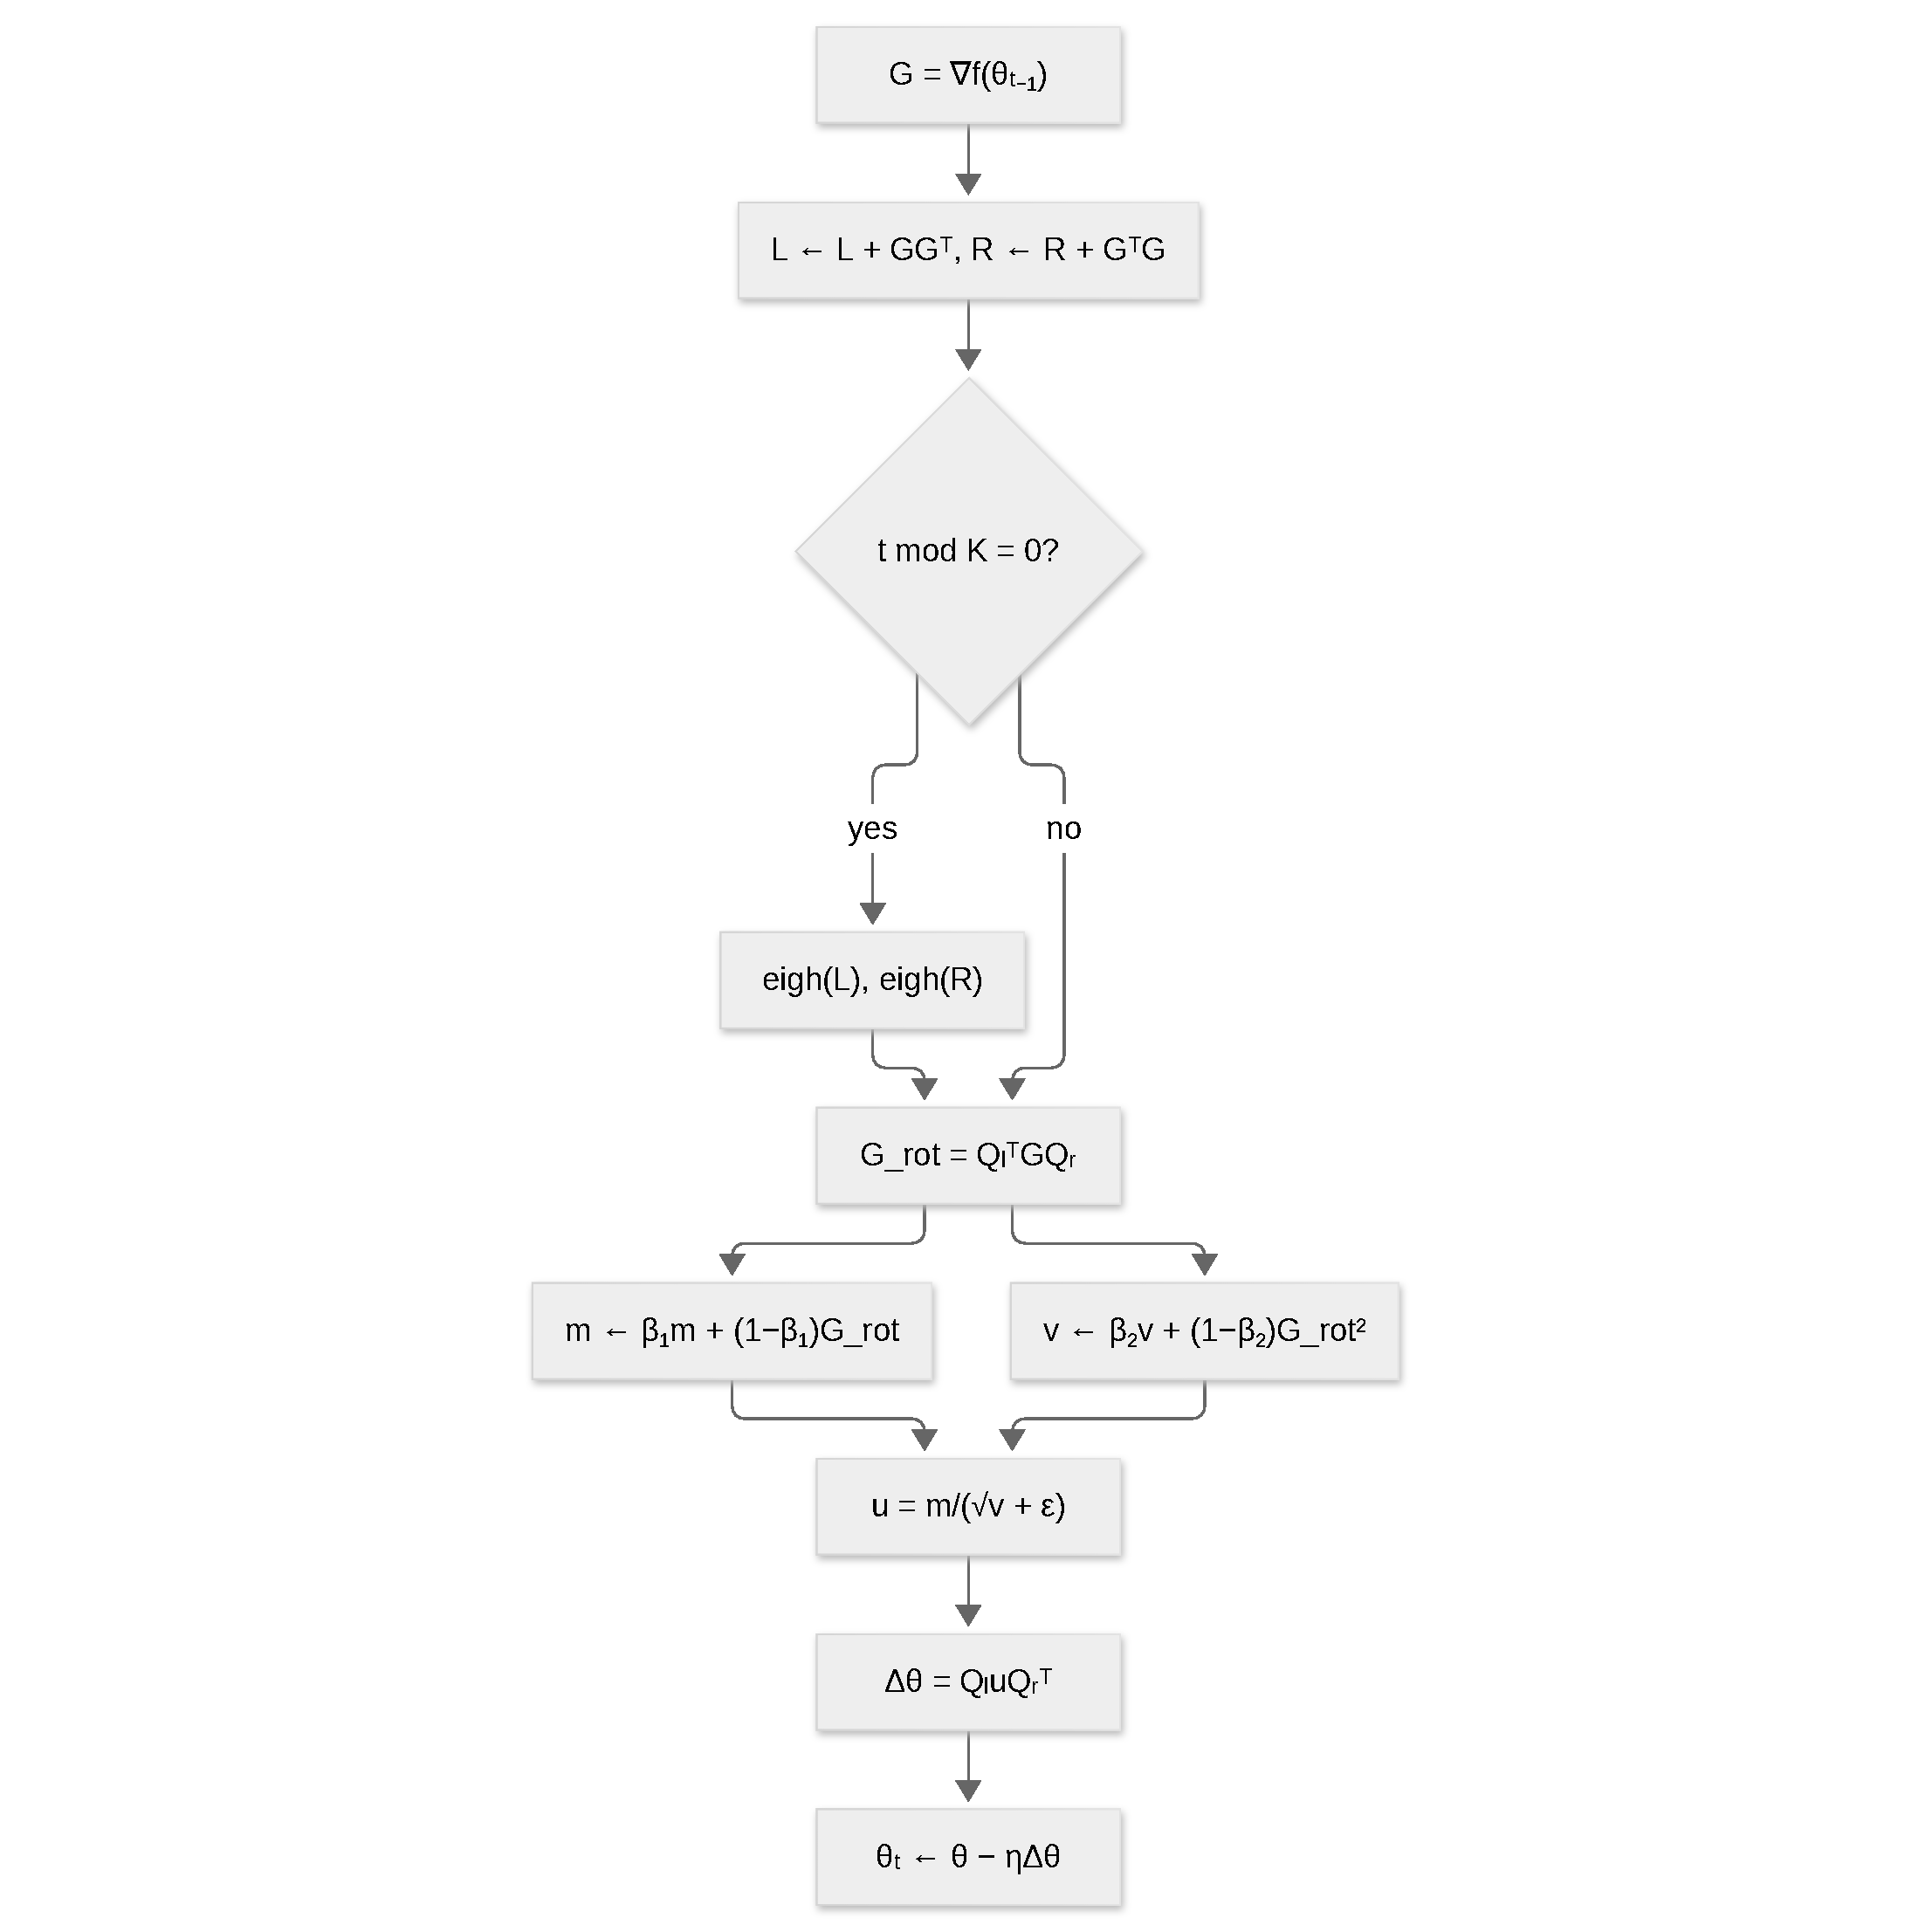
\includegraphics{figures/optimizers/soap.pdf}}
\caption{Step flow of SOAP: Adam moments tracked in the Shampoo eigenbasis and rotated back to parameter space.}
\label{fig:opt-soap}
\end{figure}
SOAP is a simplified variant of Shampoo that decouples preconditioning from momentum tracking. Instead of complex matrix algebra on preconditioned gradients, SOAP runs standard Adam in the eigenbasis of Shampoo's preconditioners:
\begin{align}
L_t &= L_{t-1} + G_t G_t^\top, \quad R_t = R_{t-1} + G_t^\top G_t \quad\text{(Gram accumulation)} \\
Q_L, \Lambda_L &= \text{eigh}(L_t), \quad Q_R, \Lambda_R = \text{eigh}(R_t) \quad\text{(periodic eigendecomposition)} \\
G_t^{\text{rot}} &= Q_L^\top G_t Q_R \quad\text{(rotate gradient into eigenbasis)} \\
m_t^{\text{rot}} &= \beta_1 m_{t-1}^{\text{rot}} + (1-\beta_1) G_t^{\text{rot}} \\
v_t^{\text{rot}} &= \beta_2 v_{t-1}^{\text{rot}} + (1-\beta_2)(G_t^{\text{rot}})^2 \quad\text{(Adam in rotated space)} \\
U_t^{\text{rot}} &= \frac{m_t^{\text{rot}}}{\sqrt{v_t^{\text{rot}}}+\epsilon}, \quad U_t = Q_L U_t^{\text{rot}} Q_R^\top \quad\text{(rotate back)}
\end{align}
The key insight: all momentum tracking occurs in the well-conditioned eigenbasis, simplifying numerical stability and theoretical analysis.

\begin{algorithm}[H]
\caption{SOAP (Shampoo with Adam in Eigenbasis)}
\label{alg:soap}
\begin{algorithmic}[1]
\Require Initial parameters $\theta_0$, learning rate $\eta$, $\beta_1, \beta_2$, eigendecomposition interval $K$
\Ensure Updated parameters $\theta_T$
\State Initialize: $L \gets \epsilon I_m$, $R \gets \epsilon I_n$, $m \gets 0$, $v \gets 0$
\For{$t = 1, 2, \ldots, T$}
    \State $G \gets \nabla f(\theta_{t-1})$ \Comment{Gradient}
    \State Update Gram: $L \gets L + G G^\top$, $R \gets R + G^\top G$
    \If{$t \mod K == 0$}
        \State $Q_L, \Lambda_L \gets \text{eigh}(L)$, $Q_R, \Lambda_R \gets \text{eigh}(R)$
    \EndIf
    \State $G^{\text{rot}} \gets Q_L^\top G Q_R$ \Comment{Rotate gradient into eigenbasis}
    \State $m \gets \beta_1 m + (1-\beta_1) G^{\text{rot}}$ \Comment{Exponential moving average (bias-correct outside)}
    \State $v \gets \beta_2 v + (1-\beta_2) (G^{\text{rot}})^2$ \Comment{Second moment (bias-correct outside)}
    \State $u \gets m / (\sqrt{v} + \epsilon)$ \Comment{Adaptive step in eigenbasis}
    \State $\Delta \theta \gets Q_L u Q_R^\top$ \Comment{Rotate back to parameter space}
    \State $\theta_t \gets \theta_{t-1} - \eta \cdot \Delta \theta$
\EndFor
\Return $\theta_T$
\end{algorithmic}
\end{algorithm}

\paragraph{Cons.}
\begin{itemize}[leftmargin=*]
\item Inherits Shampoo's periodic eigendecomposition cost.
\item Rotation and inverse rotation add matrix multiplications per step.
\end{itemize}

\paragraph{Pros.}
\begin{itemize}[leftmargin=*]
\item Combines Shampoo's explicit curvature structure with Adam's proven momentum mechanics.
\item Often cleaner and more stable than full Shampoo, with eigendecompositions amortized every $K$ steps.
\end{itemize}

\paragraph{Lion (EvoLved Sign Momentum).}
\begin{figure}[H]
\centering
\fitfigure{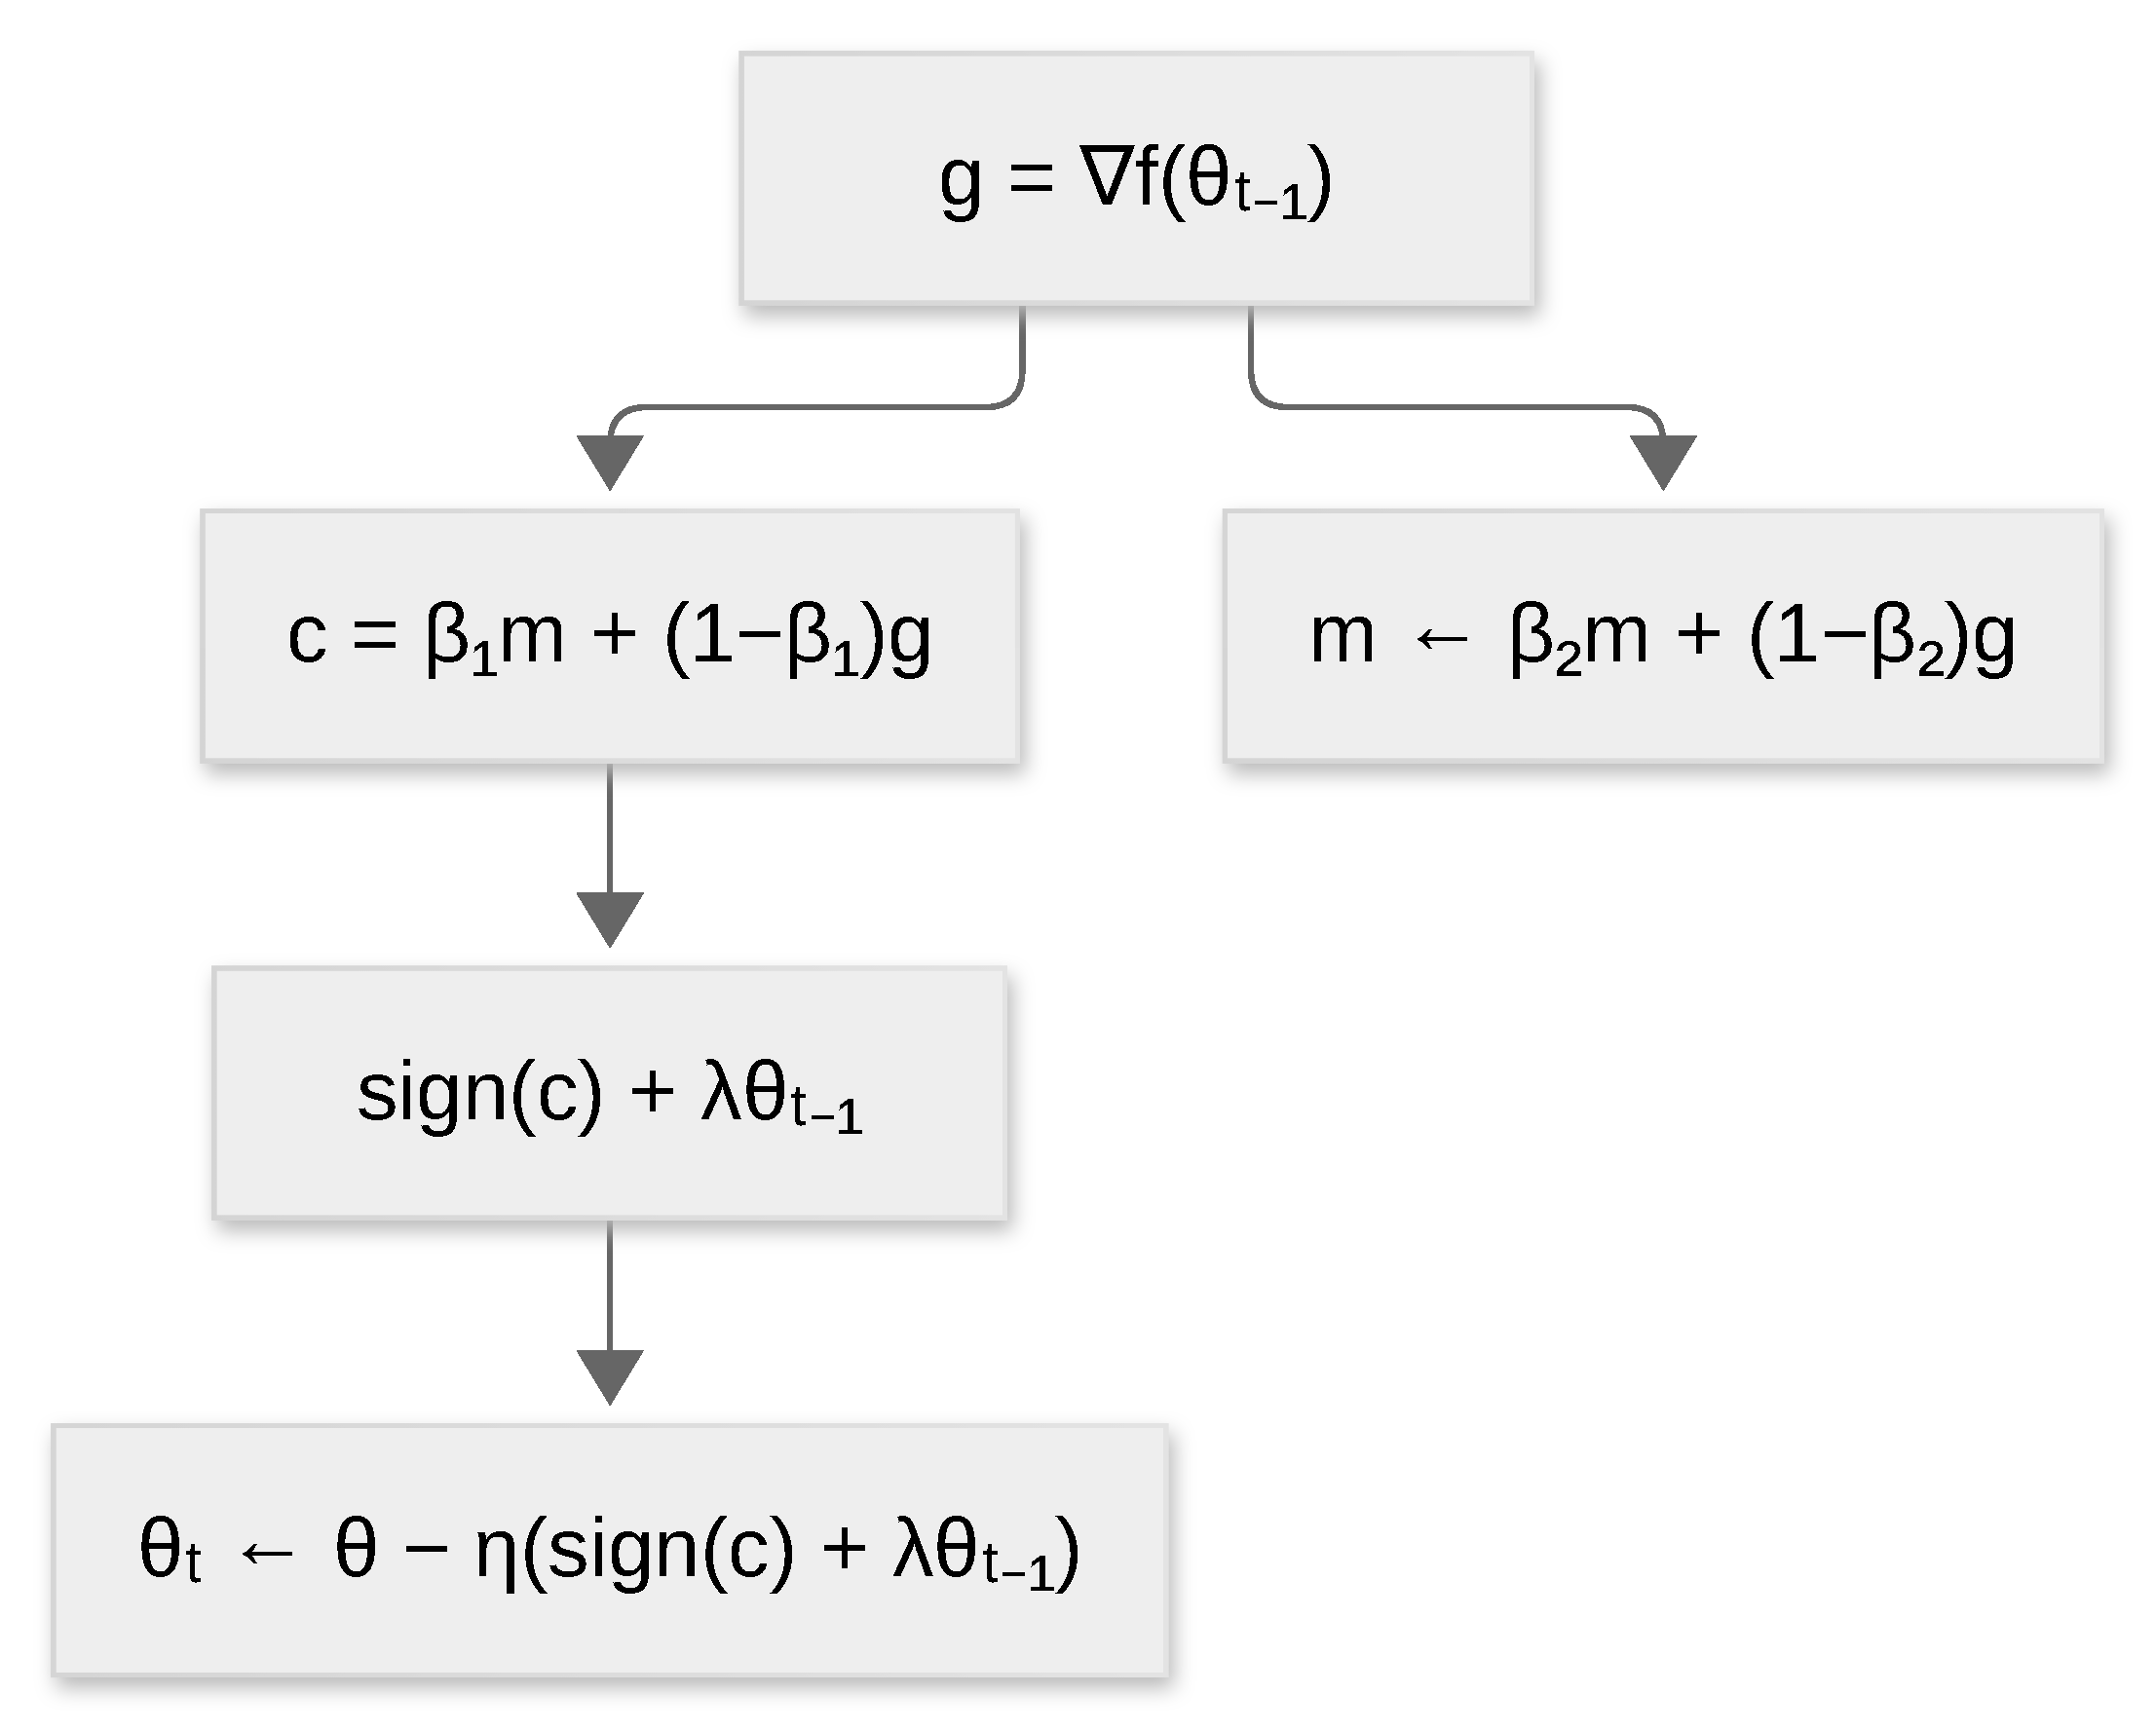
\includegraphics{figures/optimizers/lion.pdf}}
\caption{Step flow of Lion: sign-of-momentum update with decoupled momentum accumulation and weight decay.}
\label{fig:opt-lion}
\end{figure}
Lion achieves \textbf{minimal memory overhead} by using sign-based updates instead of full adaptive scaling:
\begin{align}
c_t &= \beta_1 m_t + (1-\beta_1) g_t \quad\text{(momentum input)} \\
\theta_{t+1} &= \theta_t - \eta \left(\text{sign}(c_t) + \lambda\theta_t\right) \quad\text{(sign operator update)} \\
m_{t+1} &= \beta_2 m_t + (1-\beta_2) g_t \quad\text{(momentum accumulation)}
\end{align}
All element-wise scaling operations are replaced with \texttt{sign()}, which outputs $\{-1, 0, +1\}$. This dramatically reduces memory compared to Adam-like methods: Lion stores only the momentum buffer, no second moment variance.

\begin{algorithm}[H]
\caption{Lion (EvoLved Sign Momentum)}
\label{alg:lion}
\begin{algorithmic}[1]
\Require Initial parameters $\theta_0$, learning rate $\eta$, $\beta_1, \beta_2$, weight decay $\lambda$
\Ensure Updated parameters $\theta_T$
\State Initialize: $m \gets 0$ (momentum buffer)
\For{$t = 1, 2, \ldots, T$}
    \State $g \gets \nabla f(\theta_{t-1})$ \Comment{Gradient}
    \State $c \gets \beta_1 m + (1-\beta_1) g$ \Comment{Momentum input}
    \State $\theta_t \gets \theta_{t-1} - \eta (\text{sign}(c) + \lambda \theta_{t-1})$ \Comment{Sign-based update with weight decay}
    \State $m \gets \beta_2 m + (1-\beta_2) g$ \Comment{Momentum accumulation (decoupled)}
\EndFor
\Return $\theta_T$
\end{algorithmic}
\end{algorithm}

\paragraph{Cons.}
\begin{itemize}[leftmargin=*]
\item Sign-based updates sacrifice the element-wise learning-rate adaptation that makes Adam effective.
\item Can be less robust than Adam-family methods on tasks that need adaptive scaling.
\end{itemize}

\paragraph{Pros.}
\begin{itemize}[leftmargin=*]
\item Stores only the momentum buffer, with no second moment variance.
\item High-throughput, low-memory option for large-batch regimes where activation memory dominates.
\end{itemize}

\paragraph{Sophia (Second-Order Hessian Information with Optimized Approximation).}
\begin{figure}[H]
\centering
\fitfigure{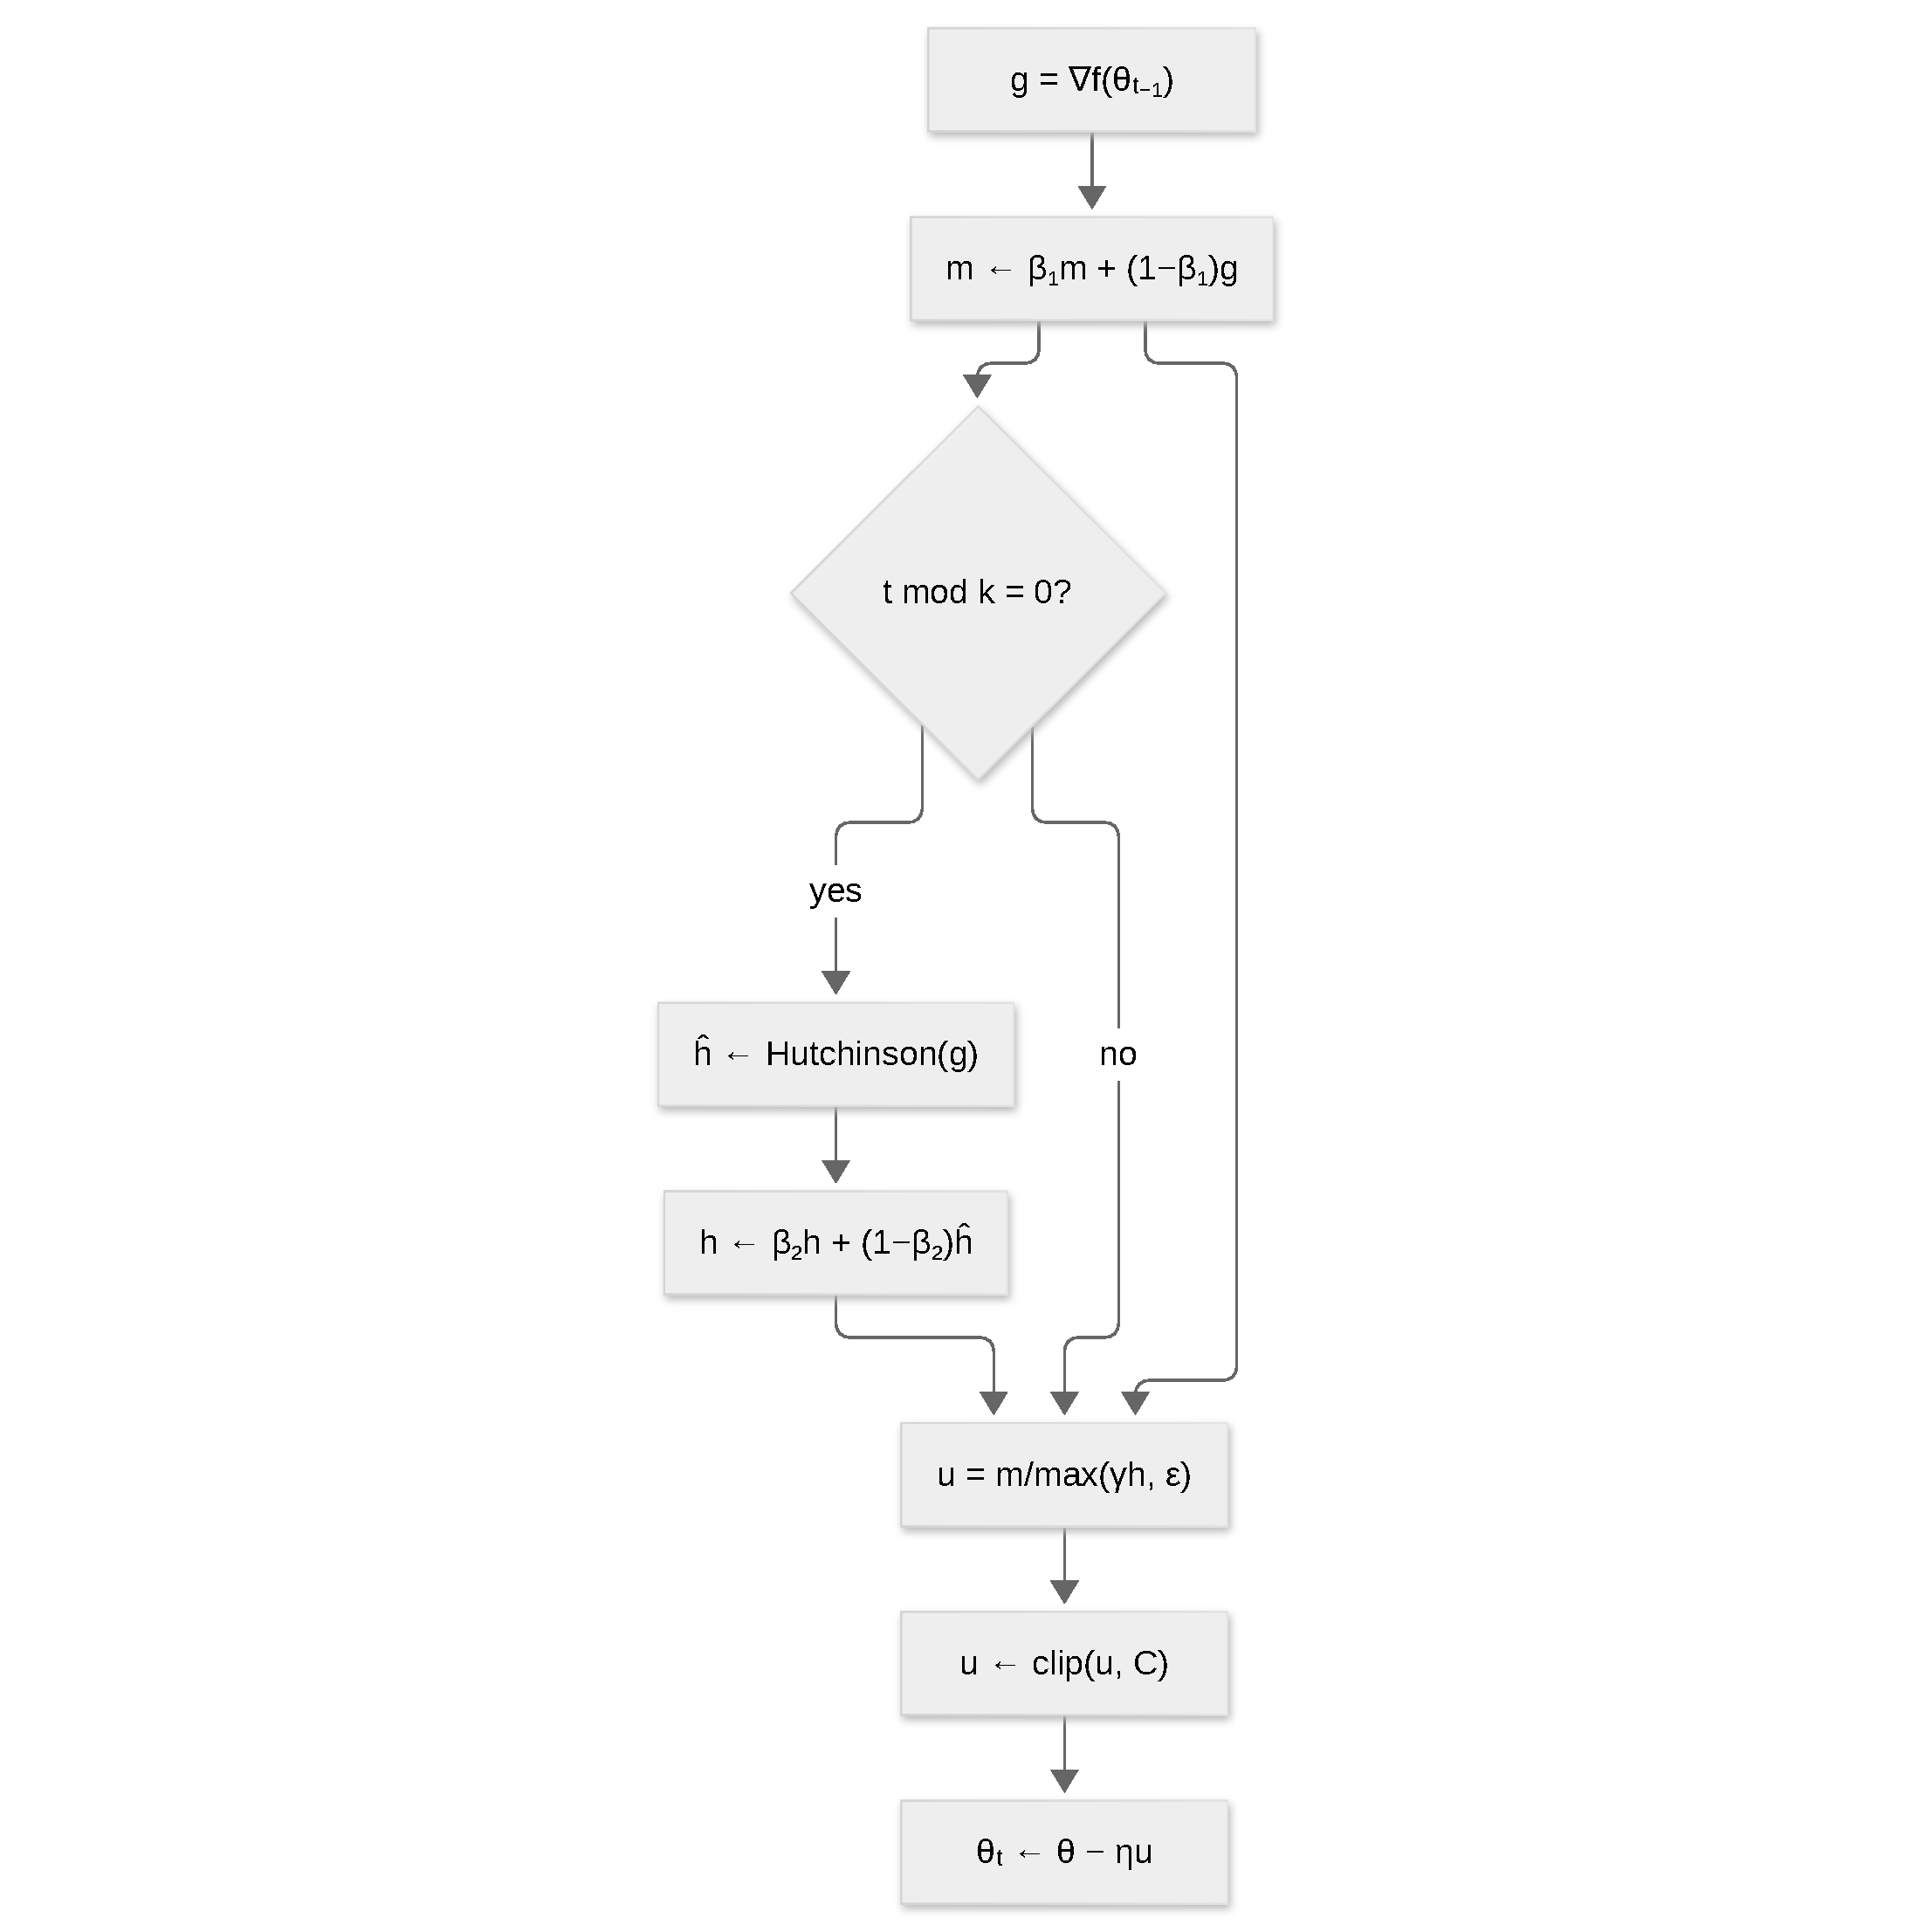
\includegraphics{figures/optimizers/sophia.pdf}}
\caption{Step flow of Sophia: diagonal Hutchinson Hessian estimate with clipped, curvature-aware element-wise steps.}
\label{fig:opt-sophia}
\end{figure}
Sophia uses \textbf{diagonal Hessian estimates} for curvature-aware scaling without the memory and compute cost of dense second-order methods.
\begin{align}
m_t &= \beta_1 m_{t-1} + (1-\beta_1) g_t \quad\text{(first moment)} \\
h_t &= \beta_2 h_{t-(k-1)} + (1-\beta_2) \hat{h}_t \quad\text{(diagonal Hessian, updated every $k$ steps)} \\
\text{clip}(x, C) &= \min(\max(x, -C), C) \quad\text{(element-wise clipping)} \\
\theta_{t+1} &= \theta_t - \eta \cdot \text{clip}\left(\frac{m_t}{\max(\gamma h_t, \epsilon)}, 1\right)
\end{align}
where $\hat{h}_t$ is a diagonal estimate (e.g., Hutchinson-trace estimator) and $\gamma$ is a scaling factor. The diagonal Hessian $h_t$ captures local curvature, allowing the optimizer to take smaller steps in sharp directions and larger steps in flat directions. The clipping operation $\text{clip}(\cdot, 1)$ prevents adaptive steps from exploding.

\begin{algorithm}[H]
\caption{Sophia (Diagonal Hessian with Clipped Updates)}
\label{alg:sophia}
\begin{algorithmic}[1]
\Require Initial parameters $\theta_0$, learning rate $\eta$, $\beta_1, \beta_2$, Hessian update freq $k$, clip threshold $C$
\Ensure Updated parameters $\theta_T$
\State Initialize: $m \gets 0$, $h \gets \epsilon$ (diagonal Hessian estimate)
\For{$t = 1, 2, \ldots, T$}
    \State $g \gets \nabla f(\theta_{t-1})$
    \State $m \gets \beta_1 m + (1-\beta_1) g$ \Comment{First moment (bias-correct outside)}
    \If{$t \mod k == 0$}
        \State $\hat{h} \gets \text{HutchinsonEstimate}(g)$ \Comment{Diagonal Hessian via Hutchinson}
        \State $h \gets \beta_2 h + (1-\beta_2) \hat{h}$ \Comment{Update Hessian estimate}
    \EndIf
    \State $u \gets \frac{m}{\max(\gamma h, \epsilon)}$ \Comment{Adaptive step (element-wise)}
    \State $u \gets \text{clip}(u, C)$ \Comment{Element-wise clipping to $[-C, C]$}
    \State $\theta_t \gets \theta_{t-1} - \eta \cdot u$
\EndFor
\Return $\theta_T$
\end{algorithmic}
\end{algorithm}

\paragraph{Cons.}
\begin{itemize}[leftmargin=*]
\item Hutchinson estimates add periodic compute and noise to the curvature signal.
\item The Hessian estimate can become stale between refreshes.
\end{itemize}

\paragraph{Pros.}
\begin{itemize}[leftmargin=*]
\item Curvature-aware scaling without the $O(n^2)$ or $O(n^3)$ cost of full second-order methods.
\item Clipped steps prevent explosions and work particularly well in second-pass fine-tuning.
\end{itemize}

\paragraph{Muon (Newton-Schulz Orthogonalization).}
\begin{figure}[H]
\centering
\fitfigure{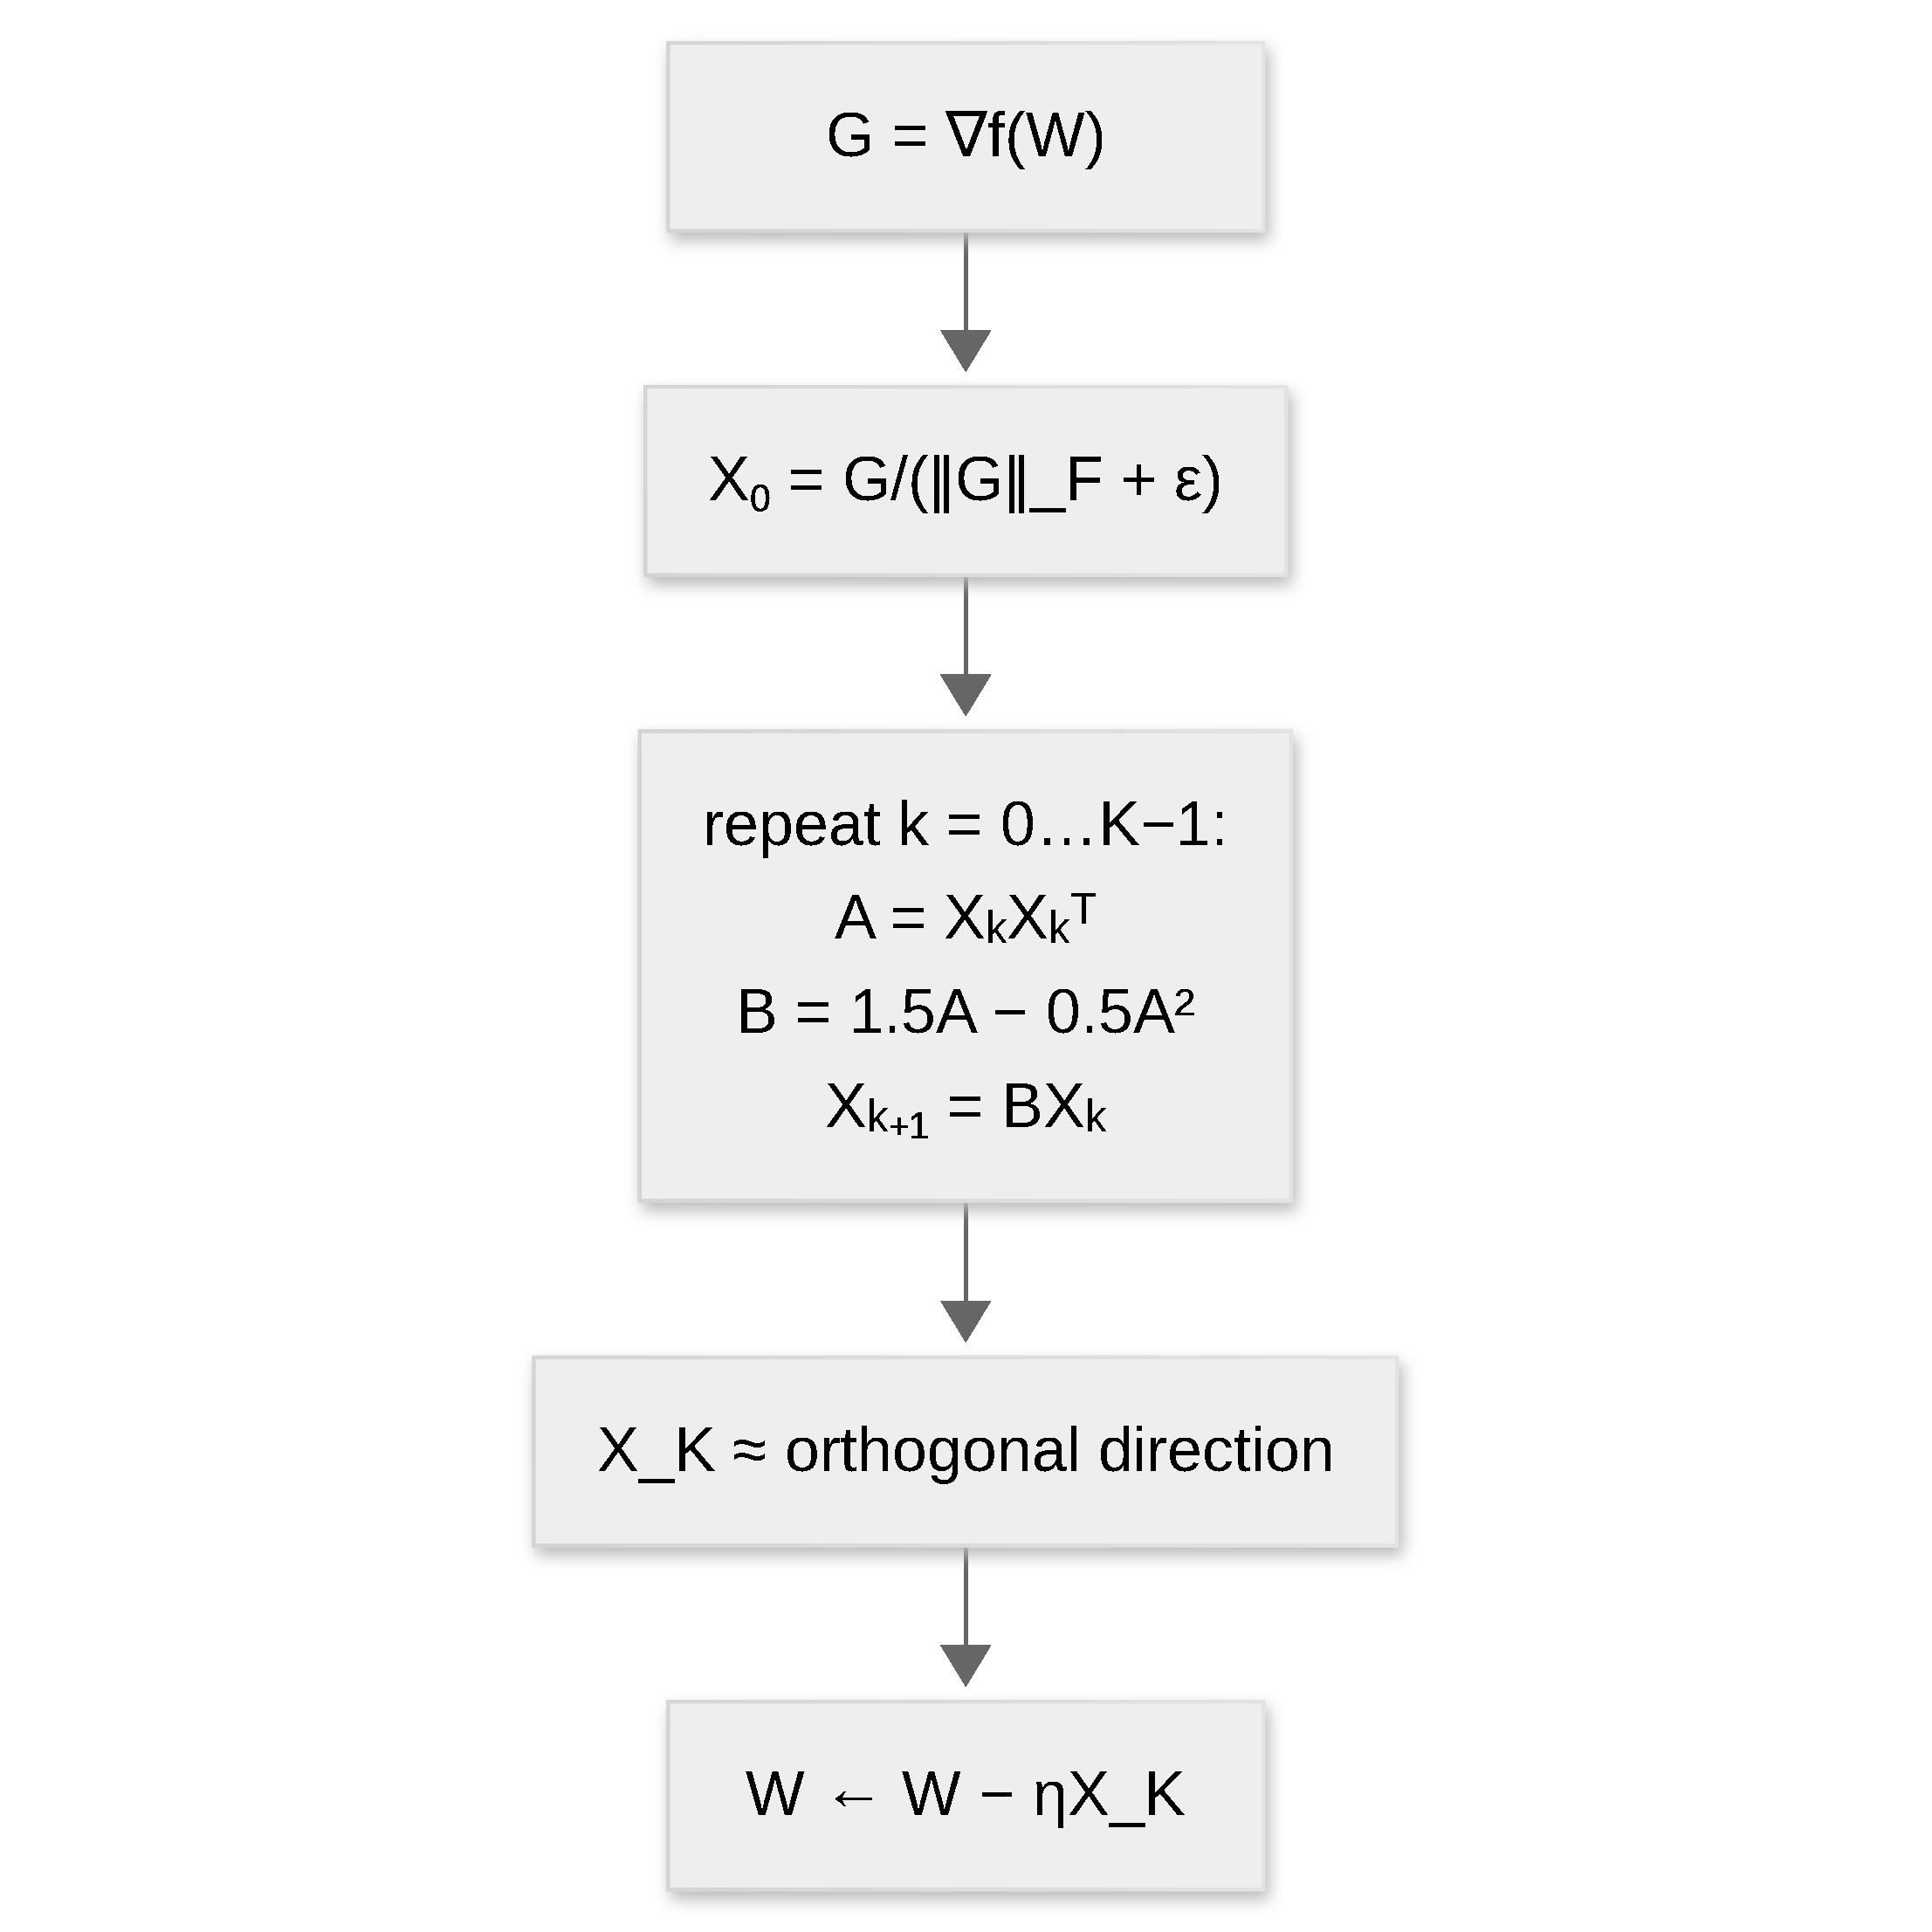
\includegraphics{figures/optimizers/muon.pdf}}
\caption{Step flow of Muon: Frobenius normalization followed by Newton-Schulz iterations that orthogonalize the update direction.}
\label{fig:opt-muon}
\end{figure}
Muon is an \textbf{orthogonality-oriented optimizer} that reshapes update geometry using Newton-Schulz polynomial iterations for orthogonalization. For a 2D parameter matrix $W$ with gradient $G_t$:
\begin{align}
X_0 &= \frac{G_t}{\|G_t\|_F + \epsilon} \quad\text{(normalized gradient)} \\
A_k &= X_k X_k^\top \quad\text{(Gramian)} \\
B_k &= b A_k + c A_k^2 \quad\text{(polynomial step, coefficients $b, c$ from Newton-Schulz)} \\
X_{k+1} &= a X_k + B_k X_k \quad\text{(iteration $k=0,1,\ldots,4$)} \\
W_{t+1} &= W_t - \eta X_K \quad\text{(update with orthogonalized direction)}
\end{align}
Muon performs 5 Newton-Schulz iterations to produce an approximately orthogonal direction, ensuring updates respect geometric constraints. The rationale: orthogonal updates preserve norms during training, avoiding the norm creep observed in momentum-based methods.

\begin{algorithm}[H]
\caption{Muon (Newton-Schulz Orthogonalization)}
\label{alg:muon}
\begin{algorithmic}[1]
\Require Initial parameters $\theta$ (matrices), learning rate $\eta$, Newton-Schulz iters $K$
\Ensure Updated parameters $\theta_T$
\For{each 2D parameter matrix $W$}
    \State $G \gets \nabla f(W)$ \Comment{Gradient}
    \State $X_0 \gets \frac{G}{\|G\|_F + \epsilon}$ \Comment{Normalize gradient by Frobenius norm}
    \For{$k = 0, 1, \ldots, K-1$}
        \State $A_k \gets X_k X_k^\top$ \Comment{Gramian (cost: $O(mn^2)$ or $O(m^2n)$ for tall/wide)}
        \State $B_k \gets (3/2) A_k - (1/2) A_k^2$ \Comment{Newton-Schulz coefficients}
        \State $X_{k+1} \gets B_k X_k$ \Comment{Polynomial step}
    \EndFor
    \State $W \gets W - \eta X_K$ \Comment{Update with orthogonalized direction}
\EndFor
\Return $\theta_T$
\end{algorithmic}
\end{algorithm}

\paragraph{Cons.}
\begin{itemize}[leftmargin=*]
\item Several matrix multiplications per Newton-Schulz iteration; efficient custom kernels are required.
\item Defined only for 2D parameter matrices.
\end{itemize}

\paragraph{Pros.}
\begin{itemize}[leftmargin=*]
\item Orthogonalized updates preserve norms and avoid the norm creep of momentum-based methods.
\item Promising results on large-scale training with fundamentally better-conditioned update geometry.
\end{itemize}

\paragraph{Turbo-Muon (AOL-Preconditioned Orthogonalization).}
\begin{figure}[H]
\centering
\fitfigure{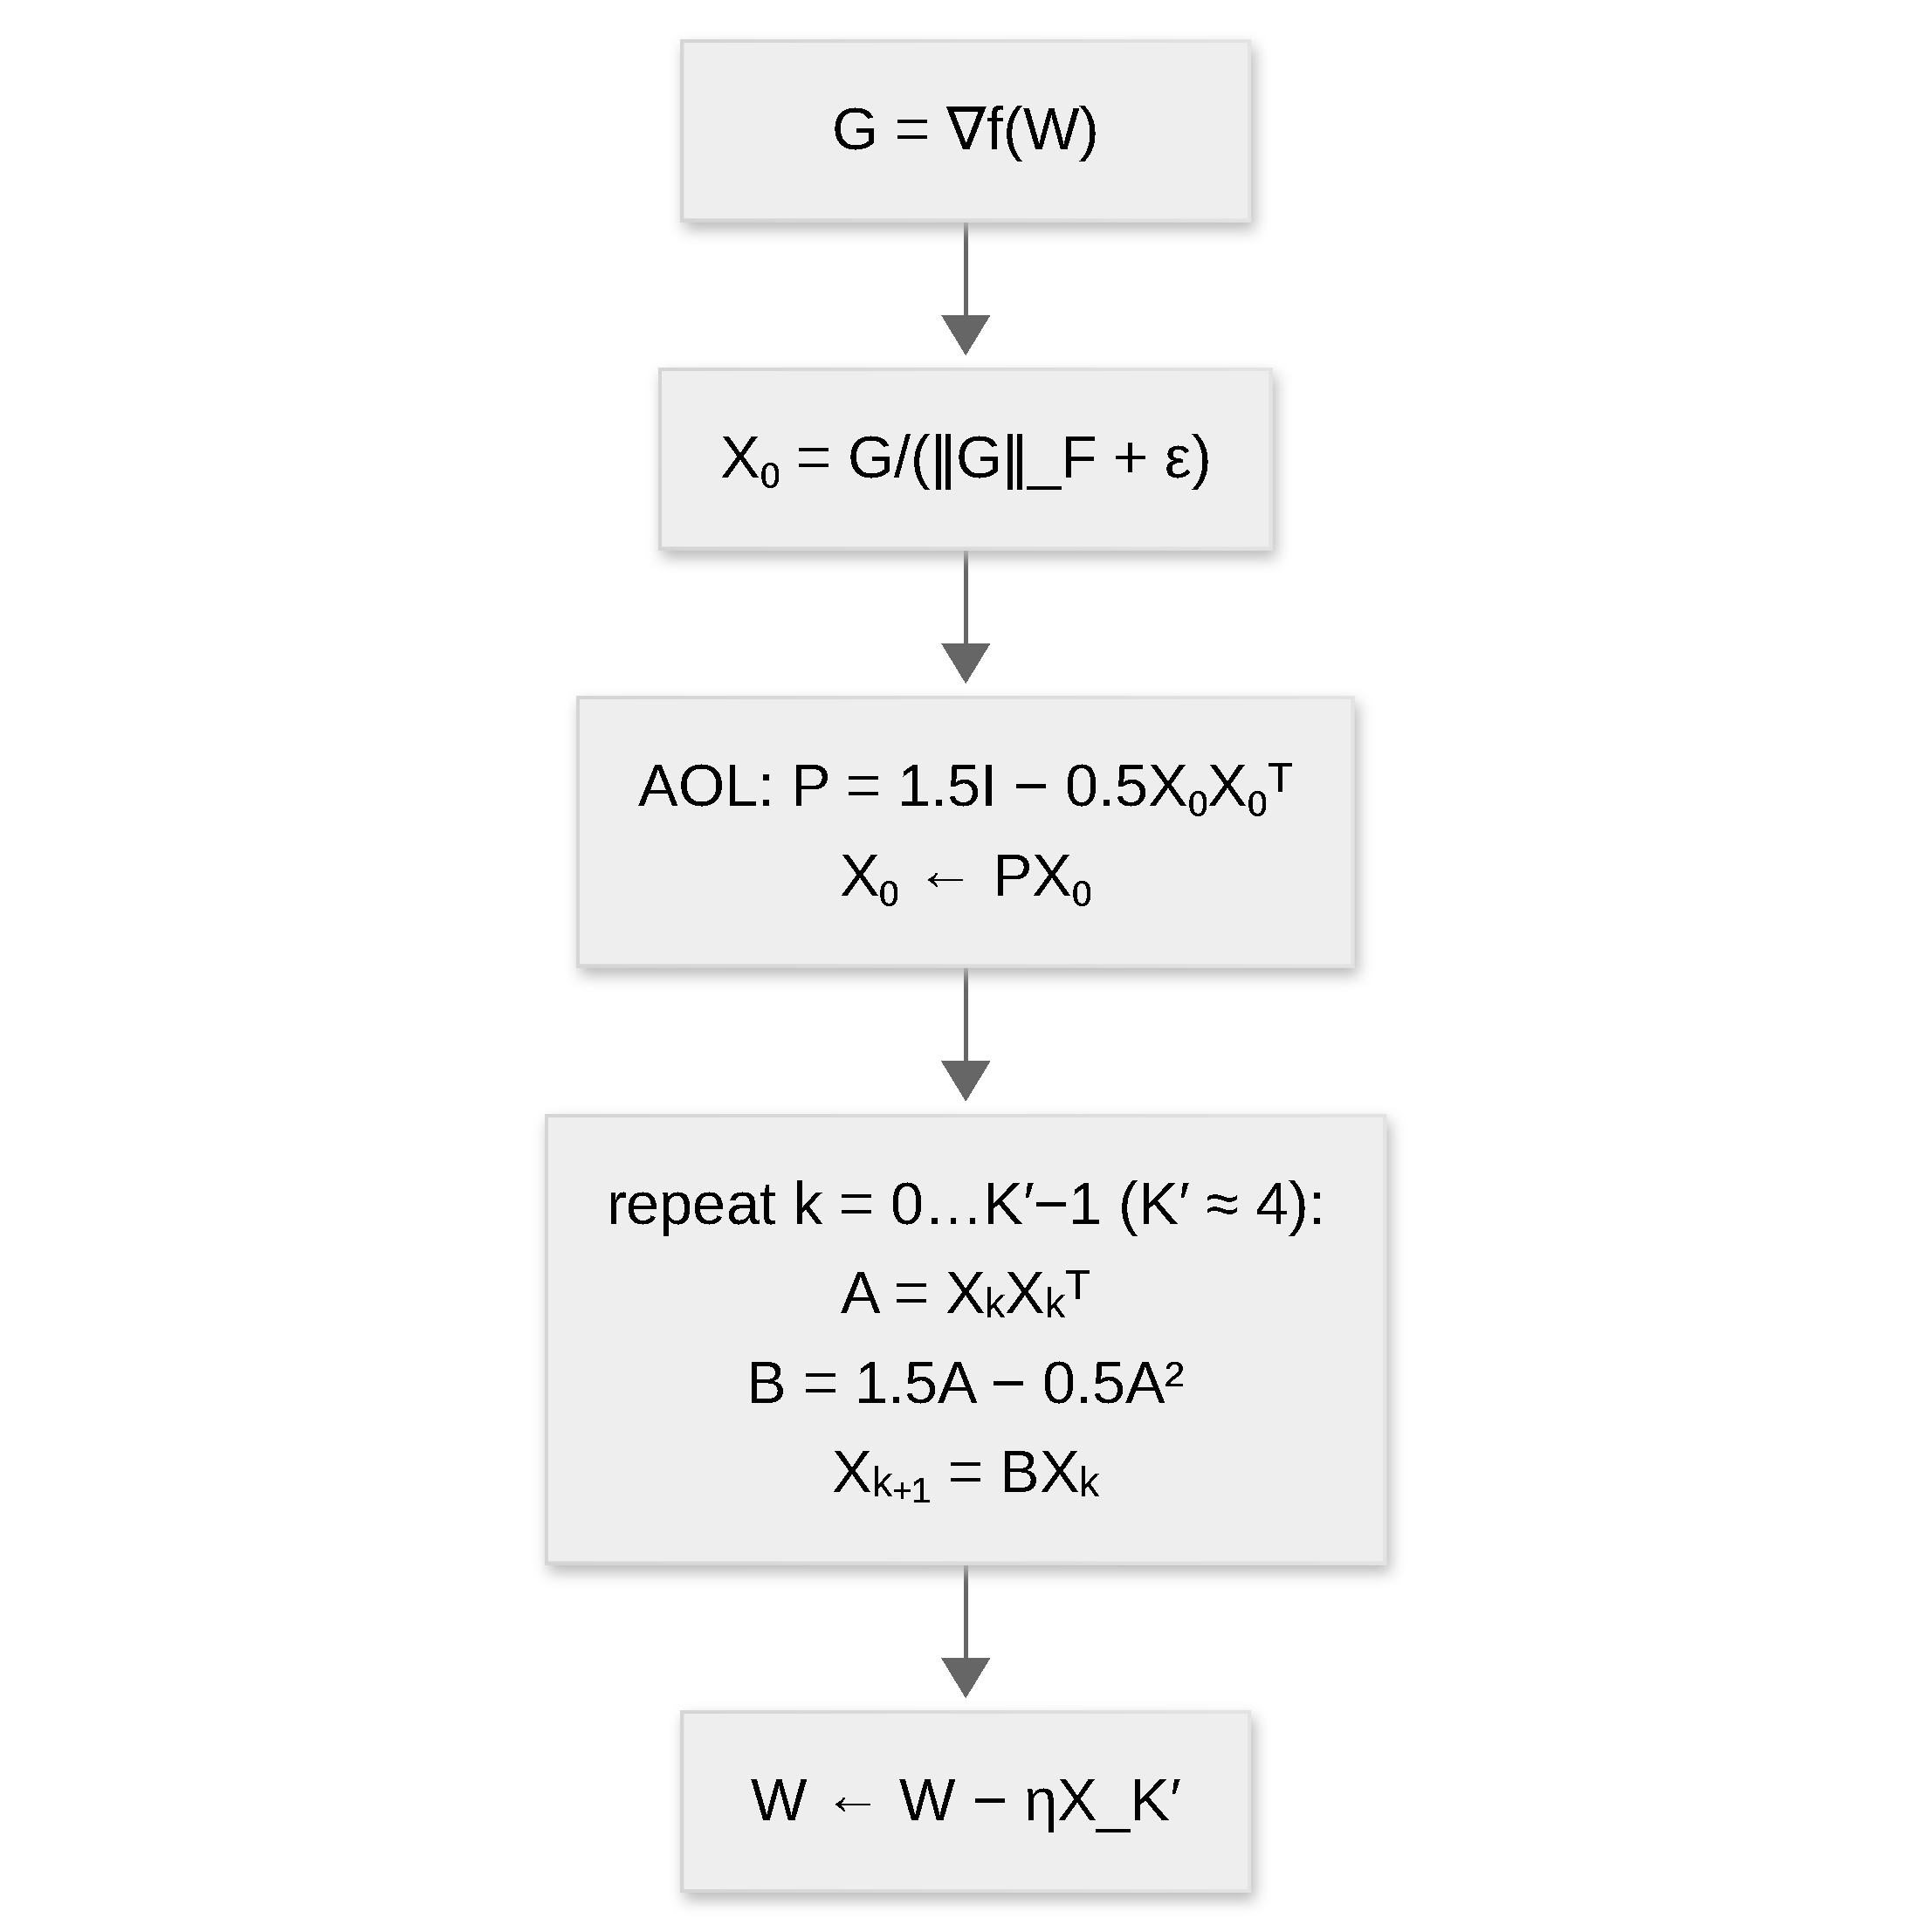
\includegraphics{figures/optimizers/turbo-muon.pdf}}
\caption{Step flow of Turbo-Muon: almost-orthogonal preconditioning (AOL) before the Newton-Schulz iterations, reducing their count.}
\label{fig:opt-turbo-muon}
\end{figure}
Turbo-Muon adds an \textbf{almost-orthogonal preconditioning} (AOL) step before the Newton-Schulz iterations. The preconditioner $P = 1.5I - 0.5X_0X_0^\top$ is applied to the normalized gradient, reducing the number of required orthogonalization steps to four while preserving the orthogonalized update geometry.

\begin{algorithm}[H]
\caption{Turbo-Muon (AOL-Preconditioned Orthogonalization)}
\label{alg:turbo-muon}
\begin{algorithmic}[1]
\Require Initial parameters $\theta$ (matrices), learning rate $\eta$, Newton-Schulz iters $K'$ (typically 4)
\Ensure Updated parameters $\theta_T$
\For{each 2D parameter matrix $W$}
    \State $G \gets \nabla f(W)$ \Comment{Gradient}
    \State $X_0 \gets \frac{G}{\|G\|_F + \epsilon}$ \Comment{Normalize gradient}
    \State \textbf{AOL (Almost-Orthogonal preconditioner):} \Comment{Preconditioning step}
    \State $P \gets (1.5 I - 0.5 X_0 X_0^\top)$ \Comment{Preconditioning matrix}
    \State $X_0 \gets P X_0$ \Comment{Preconditioned start}
    \For{$k = 0, 1, \ldots, K'-1$}
        \State $A_k \gets X_k X_k^\top$
        \State $B_k \gets (3/2) A_k - (1/2) A_k^2$
        \State $X_{k+1} \gets B_k X_k$ \Comment{Reduced iterations due to AOL preconditioning}
    \EndFor
    \State $W \gets W - \eta X_{K'}$ \Comment{Update with preconditioned orthogonalized direction}
\EndFor
\Return $\theta_T$
\end{algorithmic}
\end{algorithm}

\paragraph{Cons.}
\begin{itemize}[leftmargin=*]
\item Still compute-heavy; AOL adds a preconditioning matrix multiplication.
\item Requires the same custom-kernel support as Muon.
\end{itemize}

\paragraph{Pros.}
\begin{itemize}[leftmargin=*]
\item AOL reduces the Newton-Schulz iteration count (typically five to four).
\item Retains orthogonalized update geometry at lower iteration cost.
\end{itemize}

\paragraph{AF-Muon (AdamW-Free Tied-Embedding Muon).}
\begin{figure}[H]
\centering
\fitfigure{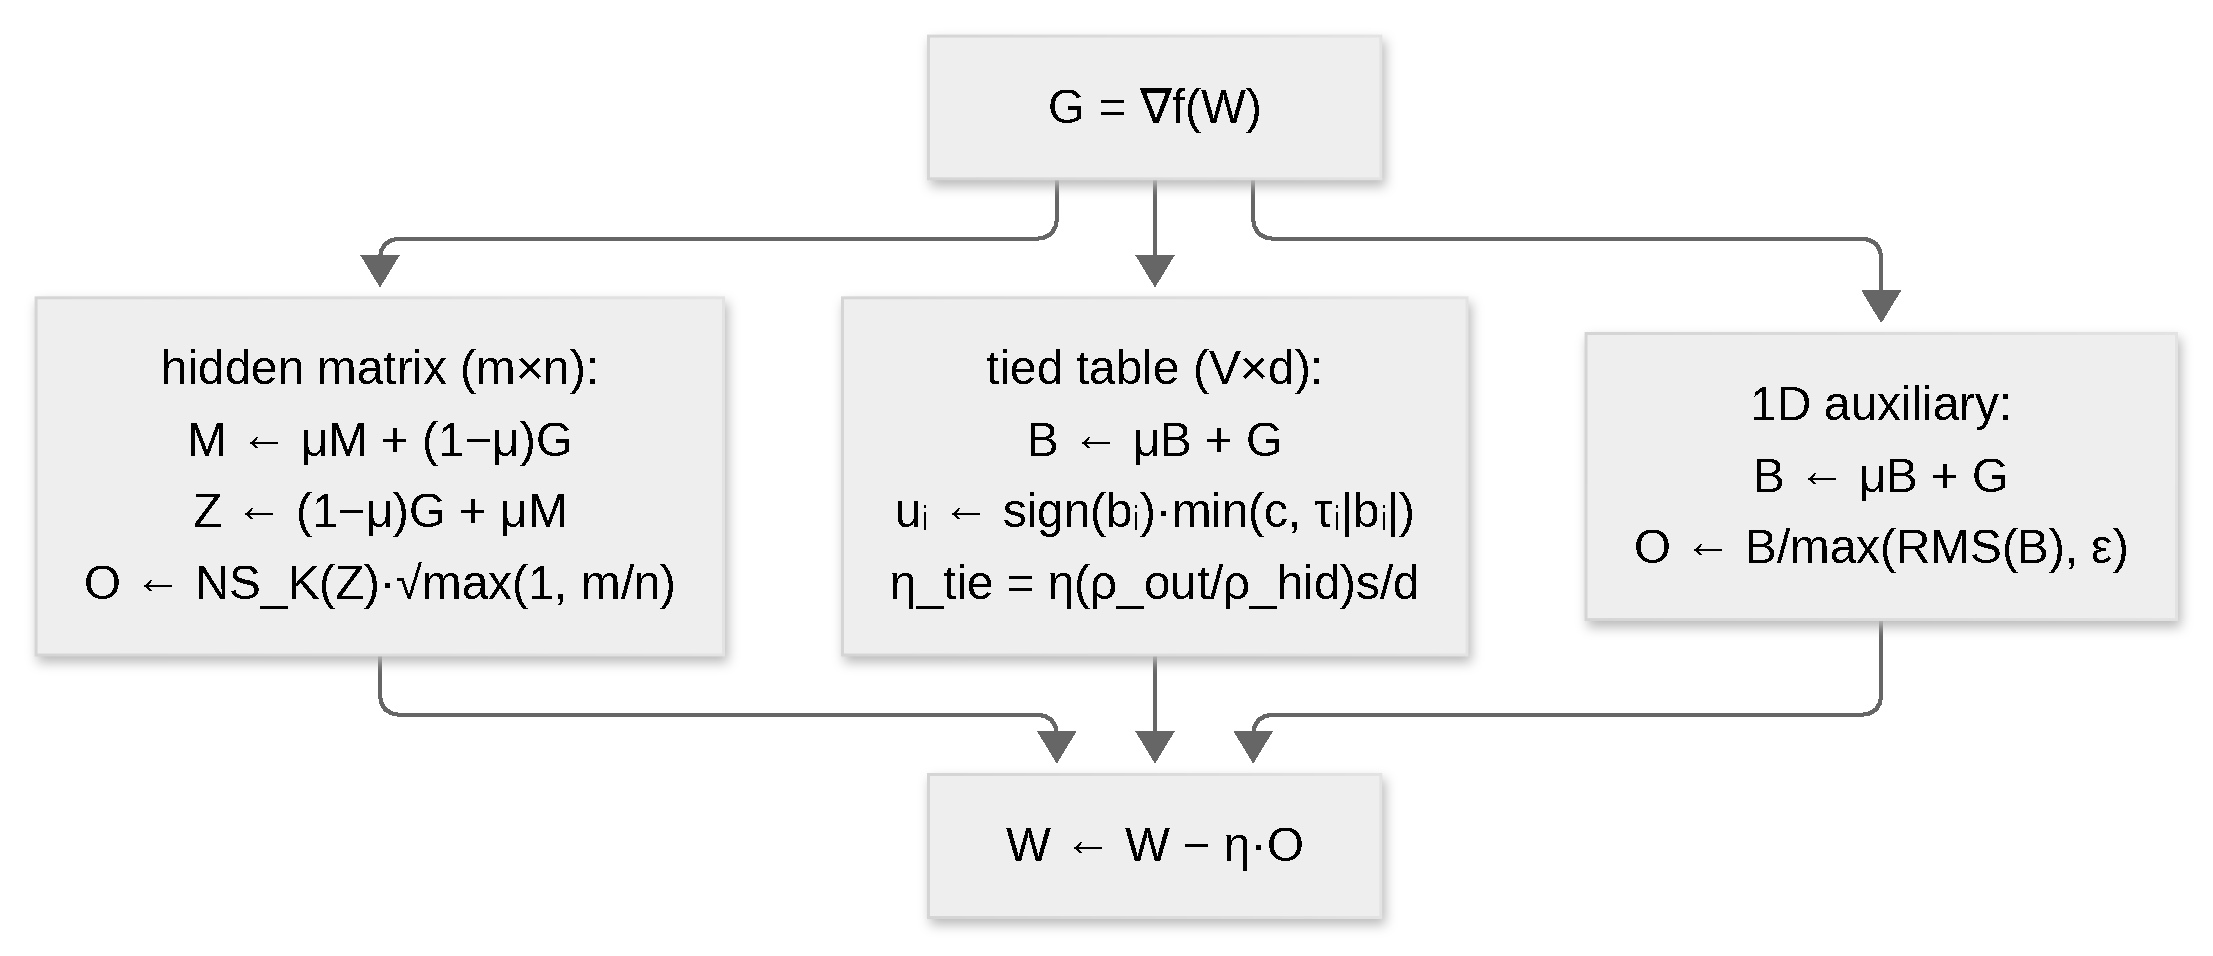
\includegraphics{figures/optimizers/af-muon.pdf}}
\caption{Step flow of AF-Muon: Muon's spectral update for hidden matrices, a support-aware finite-cap clipped-row LMO for the tied vocabulary table, and RMS-normalized updates for one-dimensional auxiliary parameters, all with a single first-moment buffer.}
\label{fig:opt-af-muon}
\end{figure}
AF-Muon is an \textbf{AdamW-free extension of Muon} that removes the auxiliary AdamW fallback of the Hybrid Muon recipe by giving every parameter class its own norm-constrained geometry. Hidden matrices keep the spectral update with a Nesterov signal; the vocabulary table, which simultaneously receives sparse input-lookup and dense output-softmax gradients, is updated row by row with a \emph{support-aware finite-cap linear minimization oracle}; one-dimensional auxiliary tensors receive an RMS-normalized update. No parameter class carries second-moment state, so a single first-moment buffer per parameter replaces the AdamW state of the hybrid recipe, which the authors report as roughly 20\% less optimizer-state memory at matched training.

For the tied table $W \in \mathbb{R}^{V \times d}$ with momentum row $b_i$, the oracle solves the row problem
\begin{align}
u_i &= \operatorname{sign}(b_i) \odot \min\left(c\,\mathbf{1},\ \tau_i\,|b_i|\right), \\
\|u_i\|_2^2 &= \min\left(d,\ c^2\,\bigl|\operatorname{supp}(b_i)\bigr|\right),
\end{align}
where the per-row scale $\tau_i$ is obtained by bisection in FP32 over complete-row chunks. Rows whose support cannot fill the row-$\ell_2$ radius saturate every useful coordinate at the cap $c$, so sparse lookup rows are handled without inflating absent coordinates. The cap interpolates between two known endpoints: $c = 1$ recovers the SCION-style Sign update and $c \geq \sqrt{d}$ reduces to a row-RMS update. The tied step size is $\eta_{tie} = \eta_M (\rho_{out}/\rho_{hid})\, s / d$; the paper's main setting is $c = 3$ and $s = 0.5$ with $\rho_{out}/\rho_{hid} = 60$, and its diagnostics report the finite cap active on under 0.3\% of coordinates while affecting most rows.

\begin{algorithm}[H]
\caption{AF-Muon (AdamW-Free Tied-Embedding Muon)}
\label{alg:af-muon}
\begin{algorithmic}[1]
\Require Initial parameters $\theta$, matrix LR $\eta_M$, vector LR $\eta_{vec}$, momentum $\mu$, matrix weight decay $\lambda_M$, tied scale $s$, cap $c$, radii $\rho_{out}, \rho_{hid}$, Newton-Schulz iters $K$
\Ensure Updated parameters $\theta_T$
\For{each parameter tensor $W$ with gradient $G_t$}
    \If{$W$ is a hidden matrix in $\mathbb{R}^{m \times n}$}
        \State $M_t \gets \mu M_{t-1} + (1-\mu) G_t$ \Comment{First moment}
        \State $Z_t \gets (1-\mu) G_t + \mu M_t$ \Comment{Nesterov signal}
        \State $O_t \gets \mathrm{NS}_K(Z_t)\sqrt{\max(1, m/n)}$ \Comment{Spectral update}
        \State $W_t \gets (1 - \eta_M \lambda_M) W_{t-1} - \eta_M O_t$
    \ElsIf{$W \in \mathbb{R}^{V \times d}$ is the tied vocabulary table}
        \State $B_t \gets \mu B_{t-1} + G_t$ \Comment{Unnormalized first moment}
        \State $\eta_{tie,t} \gets \eta_M (\rho_{out}/\rho_{hid}) s / d$
        \For{each row $i = 1, \ldots, V$}
            \State $u_i \gets L_c\bigl(\mathrm{row}_i(B_t)\bigr)$ \Comment{Capped-row LMO}
        \EndFor
        \State $W_t \gets W_{t-1} - \eta_{tie,t} U$
    \Else
        \State $B_t \gets \mu B_{t-1} + G_t$ \Comment{$1$D auxiliary tensor}
        \State $O_t \gets B_t / \max(\mathrm{RMS}(B_t), \epsilon)$
        \State $W_t \gets W_{t-1} - \eta_{vec} O_t$
    \EndIf
\EndFor
\Return $\theta_T$
\end{algorithmic}
\end{algorithm}

\paragraph{Cons.}
\begin{itemize}[leftmargin=*]
\item Every parameter must be assigned an explicit role (matrix, tied table, or vector); an untied output head or an extra embedding table is not a tied-table block.
\item The tied-table oracle requires a per-row bisection with complete-row chunking; the paper reports roughly 1\% median step-time overhead at matched training.
\item The tied-table claim is established for tied-vocabulary models; frontier-scale pretraining and universal endpoint superiority are not claimed.
\end{itemize}

\paragraph{Pros.}
\begin{itemize}[leftmargin=*]
\item AdamW-free: one first-moment buffer per parameter and no second-moment state, reported as roughly 20\% less optimizer-state memory than Hybrid Muon.
\item The finite cap preserves within-row magnitudes while bounding coordinate concentration, and recovers Sign ($c=1$) and row-RMS ($c \geq \sqrt{d}$) as limit cases.
\item Improves mean validation loss and perplexity over both Hybrid Muon and a SCION-style Sign endpoint across nine tied-token settings spanning text, image-token, protein, MoE, and encoder-decoder models.
\end{itemize}

\small
\begin{longtable}{L{2.5cm}L{3.5cm}L{2.3cm}L{5.0cm}}
\toprule
\textbf{Group} & \textbf{Methods} & \textbf{Primary Goal} & \textbf{Interpretation from the Survey} \\
\midrule
\endhead
Classical baseline & SGD, AdamW, RAdam & stability and reference baselines & These define the comparison floor for newer optimizer claims. \\
Momentum redesign & Adan, AdEMAMix, MARS, Cautious AdamW & faster or safer first-order adaptation & Best when convergence speed or noisy-gradient stability is the main concern. \\
Large-batch and schedule simplification & LAMB, Schedule-Free AdamW & operational robustness at scale & Reduce brittleness from batch-size growth or schedule engineering. \\
Memory-efficient & Adafactor, GaLore, APOLLO, APOLLO-Mini, Q-APOLLO, Lion & optimizer-state reduction & Most useful when VRAM is dominated by optimizer state rather than activations; APOLLO-family methods replace dense AdamW moments with projected or quantized structured scaling. \\
Curvature-aware & Shampoo, SOAP, Sophia & better conditioning & Prefer when richer geometry is worth implementation and compute overhead. \\
Geometry-oriented & Muon, Turbo-Muon, AF-Muon & orthogonalized update structure & Specialized options for matrix geometry and representation shaping; AF-Muon assigns the tied vocabulary table a capped-row table geometry and one-dimensional parameters an RMS update, with no AdamW auxiliary state. \\
\bottomrule
\end{longtable}
\normalsize
